% arara: xelatex
% arara: xelatex
% arara: xelatex


% options:
% thesis=B bachelor's thesis
% thesis=M master's thesis
% czech thesis in Czech language
% english thesis in English language
% hidelinks remove colour boxes around hyperlinks

\documentclass[thesis=B,english, hidelinks]{FITthesis}[2019/12/23]

\usepackage{polyglossia}
\setmainlanguage{english}
\setotherlanguages{czech,slovak}


\usepackage{amsmath,amsfonts,amsthm,amssymb}
\usepackage{newpxtext,newpxmath}
% \renewcommand\chaptitlefont{\normalfont\HUGE\bfseries\rmfamily}
\addtodef\chaptitlefont{}{\rmfamily}
\addtodef\chapnumfont{}{\rmfamily}
\addtodef\chapnamefont{}{\rmfamily}

%\usepackage[utf8]{inputenc} % LaTeX source encoded as UTF-8
% \usepackage[latin2]{inputenc} % LaTeX source encoded as ISO-8859-2
% \usepackage[cp1250]{inputenc} % LaTeX source encoded as Windows-1250

% \usepackage{subfig} %subfigures
% \usepackage{amsmath} %advanced maths
% \usepackage{amssymb} %additional math symbols

\usepackage{dirtree} %directory tree visualisation
\usepackage{pdfpages}

% % list of acronyms
% \usepackage[acronym,nonumberlist,toc,numberedsection=autolabel]{glossaries}
% \iflanguage{czech}{\renewcommand*{\acronymname}{Seznam pou{\v z}it{\' y}ch zkratek}}{}
% \makeglossaries

% % % % % % % % % % % % % % % % % % % % % % % % % % % % % % 
% EDIT THIS
% % % % % % % % % % % % % % % % % % % % % % % % % % % % % % 

\department{Department of Applied Mathematics}
\title{Improving prediction of storm structure by spectral methods}
\authorGN{Adam} %author's given name/names
\authorFN{Barla} %author's surname
\author{Adam Barla} %author's name without academic degrees
\authorWithDegrees{Adam Barla} %author's name with academic degrees
\supervisor{Mgr. Petr Šimánek}
\acknowledgements{
I thank Mgr. Petr Šimánek for guiding me, offering insightful suggestions, and providing consultation during this project. Additionally, I extend my appreciation to all those who devoted their time to proofreading my thesis, including my supportive parents and my friend Aleš Sršen.
}
\abstractEN{

Short-term weather forecasting (nowcasting) is crucial in predicting extreme weather events. This thesis focuses on structural biases that can be introduced into convolutional neural network predictions.

I investigated whether guided upsampling, used instead of transposed convolution, can improve the accuracy and reliability of weather forecasts. To this end, I trained UNet and Guided UNet (GUNet) models on radar images from a network of meteorological radars created by the OPERA radar program. I analyzed both models using performance indicators such as mean squared error (MSE), mean absolute error (MAE), and the structural similarity index (SSIM).

The results showed that the GUNet model slightly outperformed the UNet model regarding average MAE and MSE and demonstrated a better ability to capture higher frequencies in the Fourier spectrum of radar images. Moreover, the GUNet model achieved marginally better results on images with higher radar echo intensity, essential for predicting severe weather events.

The study suggests that the GUNet model can improve short-term weather predictions, and the results provide a basis for further research in this area.

}

\keywordsEN{weather nowcasting, convolutional neural networks, transponed convolution, UNet, guided UNet, guided filter, guided upsampling}


\abstractCS{

Krátkodobá predpoveď počasia (nowcasting) zohráva kľúčovú úlohu pri predvídaní extrémnych výkyvov počasia. V tejto práci sa zaoberám chybami, ktoré môžu byť vnesené do predikcí konvolučných neurónových sietí.

V mojom výskume som skúmal, či aplikácia usmerneného prevzorkovania (Guided Upsampling) namiesto transponovanej konvolúcie môže zlepšiť presnosť a spoľahlivosť predpovedí počasia. Na tento účel som vytrénoval modely UNet a GUNet (Guided UNet) na radarových snímkoch zo siete meteorologických radarov vytvorených radarovým programom OPERA. Na analýzu oboch modelov som použili ukazovatele výkonnosti, ako sú stredná kvadratická chyba (MSE), stredná absolútna chyba (MAE) a index štrukturálnej podobnosti (SSIM).

Výsledky ukázali, že model GUNet mierne prekonal UNet z hľadiska priemernej strednej absolútnej chyby a strednej kvadratickej chyby. Navyše preukázal lepšiu schopnosť zachytiť vyššie frekvencie vo Fourierovom spektre radarových snímkov. Okrem toho GUNet dosahoval sčasti lepšie výsledky na snímkach s vyššou intenzitou radarového echa, čo je významné pre predpovedanie závažných poveternostných udalostí.

Na základe týchto výsledkov možno konštatovať, že model GUNet má potenciál na zlepšenie krátkodobých predpovedí počasia. Výsledky mojej práce poskytujú priestor pre ďalší výskum v tejto oblasti.
}

\keywordsCS{krátkodobá predpoveď počasia, konvolučné neurónové siete, transponovaná konvolúcia, UNet, Guided UNet, guided filter, guided upsampling}


\placeForDeclarationOfAuthenticity{Prague}
\declarationOfAuthenticityOption{1} %select as appropriate, according to the desired license (integer 1-6)
\website{https://github.com/barlaada/GUNet-nowcasting} %optional thesis URL

\usepackage[htt]{hyphenat}



\usepackage{float}

\usepackage{graphicx}
\setcounter{MaxMatrixCols}{16}
\usepackage{tikz}
\usepackage[framemethod=tikz]{mdframed}
\usetikzlibrary{arrows.meta, calc,shapes,shapes.geometric, arrows, positioning}

\usepackage{subcaption}
\usepackage{algpseudocode}
\usepackage[hang]{footmisc}
\setlength\footnotemargin{10pt}

\usepackage[acronym]{glossaries}
\makeglossaries



\definecolor{blue}{RGB}{38,139,210}
\definecolor{cyan}{RGB}{42,161,152}
\definecolor{violet}{RGB}{108,113,196}
\definecolor{red}{RGB}{220,50,47}

\definecolor{hunyadiyellow}{RGB}{237, 174, 73}
\definecolor{amaranth}{RGB}{209, 73, 91}
\definecolor{carbbeancurrent}{RGB}{0, 121, 140}
\definecolor{lapislazuli}{RGB}{48, 99, 142}
\definecolor{indigodye}{RGB}{0, 61, 91}

\definecolor{base01}{RGB}{88,110,117}
\definecolor{base02}{RGB}{7,54,66}
\definecolor{base03}{RGB}{0,43,54}


\newacronym{WMO}{WMO}{World Meteorological Organization}
\newacronym{MAE}{MAE}{Mean Absolute Error}
\newacronym{MSE}{MSE}{Mean Squared Error}
\newacronym{SSIM}{SSIM}{Structural Similarity Index Measure}
\newacronym{NN}{NN}{Neural Network}
\newacronym{CNN}{CNN}{Convolutional Neural Network}
\newacronym{GAN}{GAN}{Generative Adversarial Network}
\newacronym{GIF}{GIF}{Guided Image Filter}
\newacronym{FGF}{FGF}{Fast Guided Filter}
\newacronym{JBU}{JBU}{Joint Bilateral Upsampling}
\newacronym{GU}{GU}{Guided Upsampling}
\newglossaryentry{OPERA}
{
name=OPERA,
description={The European Operational Program for Exchange of Weather Radar Information}
}
\newacronym{TPE}{TPE}{Tree-structured Parzen Estimator}
\newacronym{GUNet}{GUNet}{Guided UNet}


\begin{document}
% \newacronym{CVUT}{{\v C}VUT}{{\v C}esk{\' e} vysok{\' e} u{\v c}en{\' i} technick{\' e} v Praze}
% \newacronym{FIT}{FIT}{Fakulta informa{\v c}n{\' i}ch technologi{\' i}}


\setsecnumdepth{part}
\chapter{Introduction}
\label{chap:introduction}

Weather forecasting has long been a critical aspect of human life, with accurate predictions allowing us to plan and protect ourselves from the potential impact of severe weather events. While long-term weather predictions offer valuable insights into general trends and patterns, they need more precision to address the immediate threats of severe storms and other fast-changing conditions.

Weather nowcasting is the practice of making short-term weather predictions on the scale of minutes to a few hours. It is a vital tool in our efforts to anticipate and respond to these rapidly evolving weather events. It is beneficial for anticipating the evolution of rapidly changing weather phenomena, like storms, thunderstorms, or heavy rainfall, which can significantly impact public safety, infrastructure, and our daily activities.

In recent years, deep learning techniques like \glspl{CNN} have significantly advanced the field of weather nowcasting, especially in predicting storm evolution using radar images. However, despite these advancements, limitations in the quality and accuracy of these predictions persist, which is the focus of my thesis.

The UNet architecture, a popular \gls{CNN} model for image processing tasks, has shown its potential in various applications, including weather nowcasting. Nonetheless, it is known to suffer from structural bias, which can introduce unwanted artifacts and reduce the quality of the predicted storm structures. To enhance the reliability and accuracy of storm structure predictions, I aim to address these issues and develop a more spectrally consistent model.

Inspired by the work of Demetris Marnerides et al. \cite{gunet}, which proposed the \gls{GUNet} architecture for high-fidelity image transformations, this thesis aims to adapt and apply the concept of spectrally consistent models to the problem of weather nowcasting.

The main objective is to investigate and remove the structural biases present in deep learning models, such as UNet, to improve the prediction of storm structures from radar images. By leveraging spectral analysis methods, I aim to identify and mitigate the adverse effects of artifacts on the predictions and examine the improvement in the prediction quality.

Initially, the thesis provides a comprehensive literature review covering weather nowcasting, convolutional neural networks, the UNet architecture, and its improvement using \gls{GU}. Then, the methodology chapter provides an introduction to the dataset of radar images produced by \gls{OPERA}, along with details about the preprocessing and data splitting techniques used on it. The chapter continues with implementation details of the UNet and the \gls{GUNet} architectures and the model training process.

The evaluation and results chapter follows, comparing the standard and improved UNet models using metrics such as \gls{MSE}, \gls{MAE}, and \gls{SSIM} while also analyzing the impact of \gls{GU} on the spectral bias. The discussion delves into the interpretation of results, limitations, potential improvements, and the implications for weather nowcasting. Finally, the thesis concludes by summarizing the findings, highlighting contributions to the field, and outlining possible future research directions.

In summary, my thesis strives to advance the field of weather nowcasting by addressing the structural biases present in deep learning models,
thereby improving the prediction of storm structures and contributing to the ongoing efforts to develop more accurate and reliable weather forecasts.

\chapter{Thesis's Objective}
\label{chap:objective}

The primary objective of this thesis is to enhance the accuracy and reliability of short-term weather predictions, notably storm structure predictions from radar images, by addressing the spectral biases present in deep learning models like the UNet architecture. By adapting and applying the \gls{GU} technique from the \gls{GUNet} architecture to weather nowcasting, the thesis aims to develop a more spectrally consistent model, effectively mitigating the adverse effects of artifacts on the predictions and contributing to the ongoing efforts to develop more accurate and reliable weather forecasts.

In the first part of the thesis, I aim to introduce the reader to \glspl{CNN} and their application in weather nowcasting. I will describe the UNet architecture, present the concept of structural bias, and discuss how it may arise and affect the network's performance. Furthermore, I will present the \gls{GU} technique and its use in the \gls{GUNet} architecture. I will also provide an overview of the dataset used for training the \glspl{NN}, characterizing its features and relevance to weather predictions.

The second part of the thesis focuses on creating a more spectrally consistent model for weather predictions using the provided dataset of radar images, which covered the area above the Czech Republic. I intend to design and implement two models, \gls{GUNet} and UNet, in PyTorch and analyze the impact of \gls{GU} on spectral bias by comparing their performance using metrics such as \gls{MSE}, \gls{MAE}, and \gls{SSIM}.


\setsecnumdepth{all}


\chapter{Literature Review}
\label{chap:literature_review}

\section{Weather Nowcasting}
\label{sec:nowcasting}


When asked to predict future rainfall, meteorologists often get it wrong. At first glance, forecasting rainfall should be manageable as it is one of the main focuses of weather predictions, but the opposite turns out to be the case. Rain is tough to forecast on a small scale.

Rainfall forms in two main ways. The first one happens when two fronts of different temperatures meet. Because of that, it is called frontal rain. The warmer air mass is lifted above, the colder as it is less dense. It then cools at a higher altitude, which causes the water trapped in the previously warmer air to condense due to a drop in the temperature. Meteorologists can predict this type of rainfall by studying these air masses using available weather instruments. Frontal rain often lasts longer and amounts to 40 percent of all rainfall.

The other 60 percent comes from a process known as convection. This type of rain happens when the ground warmed by the sun transfers heat to the nearby air. Warming can cause the air to rise to the higher layers of the atmosphere, where the water vapor condenses. Convective rainfall sounds very similar to frontal rain. Predicting precipitation accurately can be challenging due to several factors. These include determining the ground's temperature, whether the heat is enough to make the air rise, and how long the air will stay above the warm ground to absorb the heat. Knowing the amount of water vapor in the air mass is also crucial. The areas this type of rain covers are minor and likely undetectable by methods used for frontal rain predictions. Convective rain is also shorter and, therefore, harder to predict.

Weather nowcasting aims to address predictions in this shorter horizon. Keith Browning originally defined it as \textit{``the description of the current state of the weather in detail and the prediction of changes that can be expected on a timescale of a few hours''}\cite{browningnowcating}. Later, the \gls{WMO} defined \textit{nowcasting} as forecasting with local detail, by any method, over a period from the present to 6 hours ahead, including a detailed description of the current weather.

\subsection{Radars}
\label{subsec:radars}

Nowcasting is highly dependent on observational data. While surface and upper-air observations are essential, only remote sensing systems can adequately provide high-resolution spatial coverage. A weather radar is the most crucial instrument for nowcasting, particularly for severe local storms associated with thunder, lightning, heavy rain, hail, strong winds, and sudden temperature changes.

Radar has an advantage over all other observing systems in weather forcasting because it directly observes precipitation particles in three dimensions over a large area with an update rate of a few minutes. At radar ranges of less than 60 kilometers, the resolution of the precipitation is better than 1 kilometer squared. Radar makes it possible to estimate rainfall rates and amounts, observe the 3D structure of a storm, which has proven useful in estimating storm severity, and obtain the movement of storms, which is central to nowcasting. With the addition of Doppler capability\footnote{Doppler shift of the radar waves allows the radar to determine the speed and direction (only toward or away from the radar) of precipitation particles.}, it is possible to estimate the wind direction and speed. The further addition of dual-polarization\footnote{Transmitting and receiving two differently polarized waveforms.} enables differentiation of the precipitation particle type, such as rain, snow, or hail, and to identify non-precipitation echoes, such as insects and ground clutter. Dual polarization is particularly useful for data quality control. \cite{nowcastingguidlines}

The radar collects the measurements in reflectivity, a measure of the power returned to the radar, from atmospheric targets, such as raindrops, snow\-flakes, or hailstones. The radar reflectivity is measured in dBZ and is represented on a logarithmic scale in decibels (dB) to accommodate the observations in a wide range of signal strengths. The unit dBZ expresses radar reflectivity relative to a reference value (Z), which is the radar reflectivity of a 1 mm diameter droplet of water at a standard distance from the radar. The higher the radar reflectivity, the more intense the precipitation is likely to be.

Radar attributes, such as radar wavelength, Doppler capabilities, dual-polarization, sensitivity, and scanning capabilities, affect the radar's abilities. The primary one is the radar wavelength. There are three wavelengths: S-band ($\sim$10 cm), C-band ($\sim$5 cm), and X-band ($\sim$3 cm). For example, if the primary use of the radar is for estimating heavy rainfall over large regions and to warn of high-wind events from thunderstorms, then an S-band, Doppler, dual-polarization radar is the most suitable. However, if the primary use of the radar is for nowcasting snow, then C-band or even X-band may be suitable. \cite{nowcastingguidlines}

\section{Convolutional Neural Networks}
\label{sub:cnn}

\glspl{NN} are computational models inspired by biological neural networks. Their goal is to minimize errors between outputs and given target values computed by loss function, e.g., \gls{MSE}. The function is minimized by adjusting the weights inside the network based on these errors using error backpropagation and gradient descent algorithm\footnote{I will not go into the inner workings of this algorithm, as it is not the main focus of this thesis. I assume a basic understanding of forward and backward passes from the reader in feed-forward \glspl{NN}. See paper \cite{backpropagation} in which was the backpropagation first proposed.}. After a sufficient number of successive adjustments, \gls{NN} produces an output similar to the target output, and the training can be terminated based on specific criteria. \glspl{NN} can theoretically learn to represent and model any given continuous function, no matter how complex, as long as the network has an appropriate architecture and the function is well-defined within a particular domain \footnote{See paper \cite{universalapproximators}}.

\glspl{CNN} first appeared in the 90s, but their widespread use can be attributed to breakthroughs in the ImageNet image classification challenge \cite{cnn}. \glspl{CNN} have enormously impacted the world of image processing, making them a worthy candidate for predicting the weather phenomena captured in radar images. \glspl{CNN} leverage ideas, such as sparse interactions, parameter sharing, and equivariant representations, to improve machine learning systems. To understand the benefits convolutional \glspl{CNN} bring, I need to introduce a mathematical operation that makes \gls{CNN} a \gls{CNN}.

\subsection{Convolution}
\label{subsec:convolution}

Under the hood \glspl{CNN} use, as the name implies, an operation called convolution. Bread and butter of \glspl{NN} are affine transformations. Vector of inputs is received, then multiplied by some transformation matrix\footnote{A bias vector is added before passing the result to non-linear function}. These operations can be applied to various input types, such as images or sounds. Every input can be represented as a multi-dimensional array, which can then be flattened to apply the transformation. There often are dimensions along which ordering of the data matters\footnote{Width and height of images or time axis in sound}. Similarly, the data often has something we can call ``channel axis'', which represents different views of the data \footnote{Different color channels in images or audio channels in sound}. Flattening the data does not consider these relationships, which may be important in solving tasks like computer vision and speech recognition. \cite[pg. 6-8]{convolutionguide}

Discrete convolution is the answer to this concern. An excellent way to imagine the convolution operation is through a window called the kernel, sliding across the input. The input values are multiplied by the corresponding value in the overlapping window and summed up to obtain the convolution output in the window's current location. The window is then moved to the next position. Output for all valid kernel positions\footnote{Position of a kernel on top of input is valid when an input value exists for every kernel value.} is called output feature map. This whole procedure can be repeated with many more kernels to form as many output feature maps as desired. In figure \ref{fig:convolution_slide}, we see an example of convolution with 4×4 input and 3×3 kernel. From now on, I will focus on 2D convolution, in which the input and the kernel are two-dimensional.

\begin{figure}[ht]
    \centering
    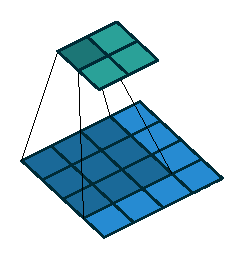
\includegraphics[width=0.24\textwidth]{images/no_padding_no_strides_00.pdf}
    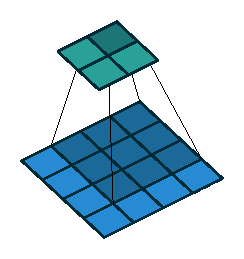
\includegraphics[width=0.24\textwidth]{images/no_padding_no_strides_01.pdf}
    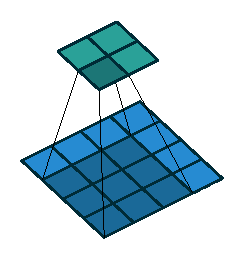
\includegraphics[width=0.24\textwidth]{images/no_padding_no_strides_02.pdf}
    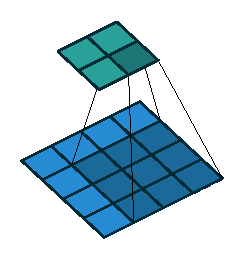
\includegraphics[width=0.24\textwidth]{images/no_padding_no_strides_03.pdf}
    \caption[2D convolution with 4×4 and 3×3 kernel]{\label{fig:convolution_slide}
    Convolving a 3×3 kernel over a 4×4 input. \cite{convolutionguide}}
\end{figure}

There can be several feature maps in the input, e.g., representing different image color channels. In that case, the kernel can have multiple dimensions. Using a multi-dimensional kernel is equivalent, to creating the output feature map, by using multiple kernels and summing the resulting unique feature maps element by element. The usage of a collection of kernels to both create multiple output feature maps and convolve over input with multiple channels is illustrated in figure \ref{fig:convolution_kernel_collection}.

\begin{figure}[ht]
    \centering
    \begin{tikzpicture}[scale=.35,every node/.style={minimum size=1cm}, on grid]
        \begin{scope}[xshift=0cm,yshift=4cm]
            \begin{scope}[xshift=0cm,yshift=0cm]
                \draw[draw=base03,fill=violet,thick]
                (0,0) grid (5,5) rectangle (0,0);
            \end{scope}
            \begin{scope}[xshift=0.5cm,yshift=0.5cm]
                \draw[draw=base03,fill=blue,thick]
                (0,0) grid (5,5) rectangle (0,0);
            \end{scope}
        \end{scope}
        \foreach \y in {0,5,10} {%
            \begin{scope}[yshift=\y cm,xshift=10cm]
                \begin{scope}[xshift=0cm,yshift=0cm]
                    \draw[draw=base03,fill=violet,thick]
                    (0,0) grid (3,3) rectangle (0,0);
                \end{scope}
                \begin{scope}[xshift=0.5cm,yshift=0.5cm]
                    \draw[draw=base03,fill=blue,thick]
                    (0,0) grid (3,3) rectangle (0,0);
                \end{scope}
            \end{scope}
            \begin{scope}[yshift=\y cm,xshift=20cm]
                \begin{scope}[xshift=0.5cm]
                    \draw[draw=base03,fill=cyan,thick]
                    (0,0) grid (3,3) rectangle (0,0);
                \end{scope}
            \end{scope}
        }
        \begin{scope}[xshift=30cm,yshift=4.75cm]
            \foreach \s in {0.0,0.5,1.0} {%
            \begin{scope}[xshift=\s cm,yshift=\s cm]
                \draw[draw=base03,fill=cyan,thick]
                (0,0) grid (3,3) rectangle (0,0);
            \end{scope}
            }
        \end{scope}
        \draw[->, thick] (6, 6.25) to (9, 1.75);
        \draw[->, thick] (6, 6.75) to (9, 6.75);
        \draw[->, thick] (6, 7.25) to (9, 11.75);
        \draw[thick]  (14.5, 1.75) to (16, 1.75);
        \draw[->, thick]  (18, 1.75) to (19.5, 1.75);
        \node[thick] (p1) at (17, 1.75) {$+$};
        \draw[thick]  (14.5, 11.75) to (16, 11.75);
        \draw[->, thick]  (18, 11.75) to (19.5, 11.75);
        \node[thick] (p2) at (17, 11.75) {$+$};
        \draw[thick]  (14.5, 6.75) to (16, 6.75);
        \draw[->, thick]  (18, 6.75) to (19.5, 6.75);
        \node[thick] (p3) at (17, 6.75) {$+$};
        \draw[->, thick]  (24, 1.5) to (29.5, 6.25);
        \draw[->, thick]  (24, 6.75) to (29.5, 6.75);
        \draw[->, thick]  (24, 11.75) to (29.5, 7.25);

    \end{tikzpicture}
    \caption[2D convolution with multiple channels and kernels]{\label{fig:convolution_kernel_collection} A convolution mapping from two input feature maps to three output feature maps using three 3×3 kernel pairs $\mathbf{w}$. In the top pathway, input feature map $1$ is convolved with kernel $\mathbf{w}_{1,1}$ and input feature map 2 is convolved with kernel $\mathbf{w}_{1,2}$, and the results are summed together elementwise to form the first output feature map. The same is repeated for the middle and bottom pathways to form the second and third feature maps, and all three output feature maps are grouped to form the output.\cite{convolutionguide}}
\end{figure}

Convolution has two parameters: stride and padding. They, among other things, change the size of the output. Strides represent the size of the step that the kernel window takes when moving to the next position\footnote{Size of this step can be different in each dimension of the input.}. Padding is the ``thickness'' of a border of zeros that are added around the input\footnote{Padding can also be defined to be different in each dimension of the input.}. These parameters can be seen at work in figure \ref{fig:convolution_padding_strides}.

\begin{figure}[ht]
    \centering
    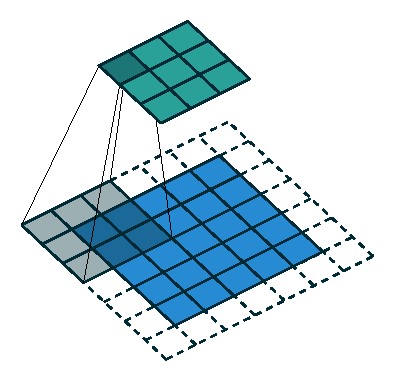
\includegraphics[width=0.24\textwidth]{images/padding_strides_00.pdf}
    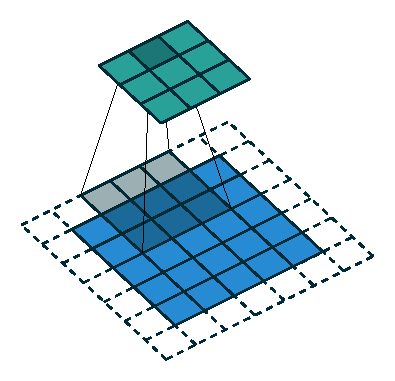
\includegraphics[width=0.24\textwidth]{images/padding_strides_01.pdf}
    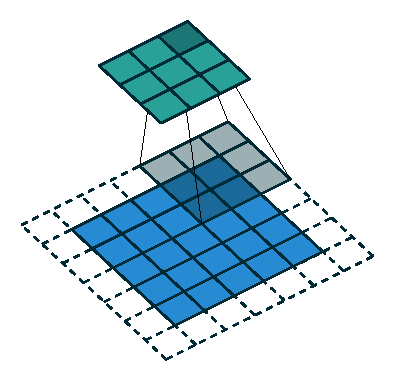
\includegraphics[width=0.24\textwidth]{images/padding_strides_02.pdf}
    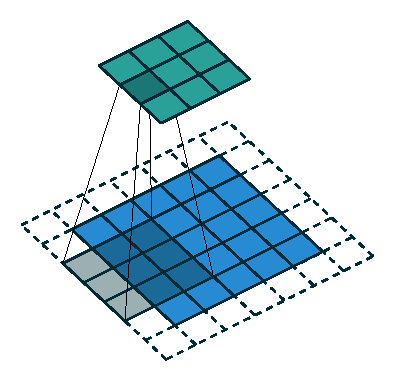
\includegraphics[width=0.24\textwidth]{images/padding_strides_03.pdf}
    \caption[2D convolution with padding and strides]{\label{fig:convolution_padding_strides}Convolving a 3×3 kernel over a 5×5 input padded with
    a 1×1 border of zeros using 2×2 strides. \cite{convolutionguide}}
\end{figure}

Convolution can also be represented as a multiplication of the input by matrix $\mathbf C $. An example of such matrix for the same case as in figure \ref{fig:convolution_slide}  can be seen in figure \ref{fig:convolution_matrix}.

\begin{figure}[ht]
    \centering
    \resizebox{0.95\hsize}{!}{$\begin{pmatrix}
        w_{0,0} & w_{0,1} & w_{0,2} & 0       & w_{1,0} & w_{1,1} & w_{1,2} & 0       & w_{2,0} & w_{2,1}   & w_{2,2}   & 0       & 0       & 0       & 0       & 0       \\
        0       & w_{0,0} & w_{0,1} & w_{0,2} & 0       & w_{1,0} & w_{1,1} & w_{1,2} & 0       & w_{2,0}   & w_{2,1}   & w_{2,2} & 0       & 0       & 0       & 0       \\
        0       & 0       & 0       & 0       & w_{0,0} & w_{0,1} & w_{0,2} & 0       & w_{1,0} & w_{1,1}   & w_{1,2}   & 0       & w_{2,0} & w_{2,1} & w_{2,2} & 0       \\
        0       & 0       & 0       & 0       & 0       & w_{0,0} & w_{0,1} & w_{0,2} & 0       & w_{1,0}   & w_{1,1}   & w_{1,2} & 0       & w_{2,0} & w_{2,1} & w_{2,2} \\
    \end{pmatrix}$}
    \caption[Convolution represented as matrix multiplication]{\label{fig:convolution_matrix}Convolution with 4×4 input and 3×3 kernel represented as matrix multiplication. Inputs and outputs are concatenated. }
\end{figure}

We can see that multiplying the input by this matrix gives us the same result as sliding the kernel window over the input. The backward pass is easily obtained from this representation by transposing $\mathbf C$. The error is backpropagated by multiplying the loss with $\mathbf C^T$.

If we look at the matrix, we can see the properties of convolution mentioned above. This representation is closer to the actual implementation used in \glspl{NN}, as it employs matrix multiplication \footnote{Software implementations will typically not perform the useless zero multiplications.}. The matrix is sparse. Therefore fewer parameters need to be stored, reducing memory requirements. It also means we can compute the convolution result faster than in the fully connected case. These efficiency improvements are pretty significant. Most algorithms used in practice run in $O(mn)$ time where $m$ and $n$ are input and output sizes, respectively. For kernel with $k$ parameters, convolution can be run in $O(kn)$ time. Speed improvement is evident when we realize that $k$ can often be orders of magnitude smaller than $m$ while obtaining a good performance.

Parameter sharing can also be seen in the matrix. Kernel weights are reused multiple times, unlike in traditional \gls{NN}, where each element of the weight matrix is used only once. Parameter sharing does not affect the forward propagation's runtime but further reduces the model's storage requirements.

Equvariance to translation is another property of \glspl{CNN}. Equivarience of function $f(x)$ to function $g$ means that $f\left(g(x)\right) = g\left(f\left(x\right)\right)$. In other words, equivariance to translation means that if I shifted the input by some number of pixels, I would get the same output but also shifted by the same amount. It is perhaps harder to see from the examples, but it is nonetheless useful. \cite[pg. 329-335]{deeplearningbook}

\gls{CNN} is defined as a \gls{NN} that has at least one convolutional layer.

\subsection{Transposed Convolution}
\label{subsec:transposed_convolution}

Transposed convolutions are quite useful, especially in generative models. The need arises from the desire to use a transformation that goes in the opposite direction of normal convolution. It is easy to assume that transposed convolution is the ``opposite'' operation of a regular convolution without giving it much thought. Its purpose is to go from something with the shape of some convolution output to something with the shape of its input. This operation should be done while maintaining a consistent connectivity pattern with said convolution. It is important to remember that there does not exist a reverse operation for convolution\footnote{Sometimes the term ``deconvolution'' is used instead of transposed convolution, which may be misleading.}. \cite{convolutionguide, deconvolutionbias}

Every convolution boils down to an efficient implementation of a matrix operation. A transposed convolution works by swapping forward and backward passes of a convolution. One kernel defines matrix $\mathbf C$, an example of which can be seen in figure \ref{fig:convolution_matrix}, and its transposition $\mathbf C^T$. The matrix used for a forward and backward pass determines the convolution type. In the transposed convolution, $\mathbf C^T$ is used for the forward pass instead of $\mathbf C$ in standard convolution.

It is always possible to emulate a transposed convolution with a direct convolution. The disadvantage is that it usually involves adding many columns and rows of zeros to the input, resulting in a much less efficient implementation. It is a more useful representation of transposed convolution. It is necessary to zero-pad the input if the same connectivity pattern, in the equivalent convolution to the transposed one, is to be maintained. It must be done so that the kernel's first (top-left) application only touches the top-left pixel.

Suppose we now imagine a convolution with non-unit strides and an ``opposite'' transposed convolution to it. In that case, the strides in the transposed convolution need to be fractional, as we are now increasing the output's size. Hence, we need to take steps smaller than one\footnote{This is why transposed convolution is sometimes also called fractionally-strided convolution.}. Fractional steps can be achieved in the representation of transposed convolution by the standard one by inserting zeros between input units. Inserting zeros between rows and columns of the input makes the kernel move around at a ``slower pace'' than with unit strides\footnote{The padding has to be equal to the size of the kernel minus one.}. Figure \ref{fig:convolution_padding_strides_transposed} illustrates the fractional strides. Transposed convolution in figure \ref{fig:convolution_padding_strides_transposed} is ``opposite'' of the convolution in figure \ref{fig:convolution_padding_strides}. \cite{convolutionguide}
\footnote{For more visualizations and a deeper explanation of how different convolution parameters, such as padding and strides, influence the output size, you can refer to \cite{convolutionguide}.}

\begin{figure}[ht]
    \centering
    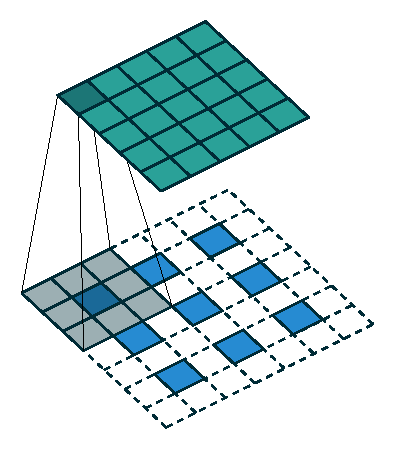
\includegraphics[width=0.24\textwidth]{images/padding_strides_transposed_00.pdf}
    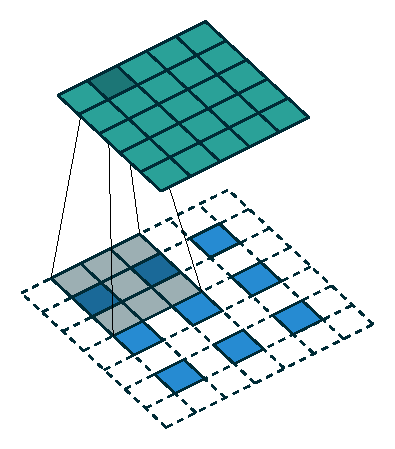
\includegraphics[width=0.24\textwidth]{images/padding_strides_transposed_01.pdf}
    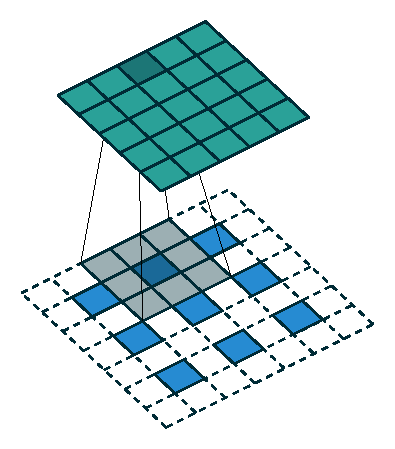
\includegraphics[width=0.24\textwidth]{images/padding_strides_transposed_02.pdf}
    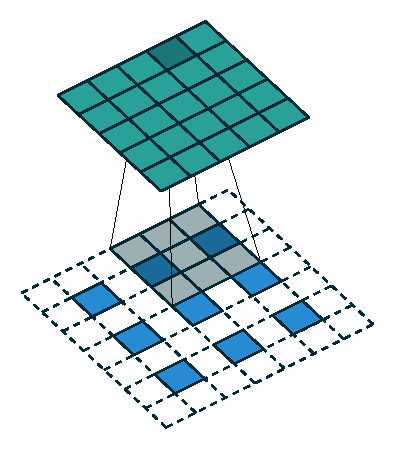
\includegraphics[width=0.24\textwidth]{images/padding_strides_transposed_03.pdf}
    \caption[2D transposed convolution]{\label{fig:convolution_padding_strides_transposed}
    Transposed convolution to convolving a 3×3 kernel over a 5×5 input padded with a 1×1 border of zeros using 2×2 strides (figure \ref{fig:convolution_padding_strides}). It is equivalent to convolving a 3×3 kernel over a 3×3 input (with
    one zero inserted between inputs) padded with a 1×1 border of zeros using unit
    strides. \cite{convolutionguide}}
\end{figure}

\subsection{Pooling}
\label{subsec:pooling}

Pooling operations reduce the size of the feature maps by using some function to summarize subregions of the input, such as taking the average or the maximum value. Pooling works like discrete convolution as it slides a window across the input, but it uses a different function instead of the linear combination used in convolution. In addition to discrete convolutions, the pooling operation makes up another vital building block in \glspl{CNN}.

\subsection{Validation Metrics}
\label{subsec:val_metrics}

Different evaluation metrics are used for assessing the performance of \glspl{CNN}, particularly in image processing and computer vision tasks. Here is a brief overview of metrics that I will use later in the thesis.
\begin{itemize}
    \item \gls{SSIM} is a perceptual metric that quantifies the similarity between two images. It considers the images' luminance, structure information, and contrast, which are more aligned with human visual perception. \gls{SSIM} values range from -1 to 1, with 1 indicating a perfect match between the two images. In the context of \glspl{NN}, \gls{SSIM} can be used to evaluate the quality of generated or reconstructed images, such as in image denoising, super-resolution, or image-to-image translation tasks.
    \item \gls{MAE} is a simple and easy-to-interpret metric that measures the average absolute difference between the predicted and actual values. It is used for both regression and image-processing tasks. For image processing, \gls{MAE} calculates the average absolute difference between the pixel values of two images. A lower \gls{MAE} indicates better model performance, which signifies fewer predicted and actual value discrepancies.
    \item \gls{MSE} is another metric used to measure the difference between predicted and actual values. It calculates the average squared difference between the two sets of values. In image processing, \gls{MSE} measures the average squared difference between the pixel values of two images. Similar to \gls{MAE}, a lower \gls{MSE} value indicates better performance. \gls{MSE} tends to penalize more significant errors more severely than MAE, as the squared term magnifies the differences.
\end{itemize}

Figure \ref{fig:metric} captures differences between each metric. These metrics are used to evaluate and compare the performance of different neural network models or configurations in various tasks, such as image synthesis, denoising, segmentation, and more. Models can be fine-tuned to achieve better results by analyzing the performance using these metrics.

\begin{figure}[ht]
    \centering
    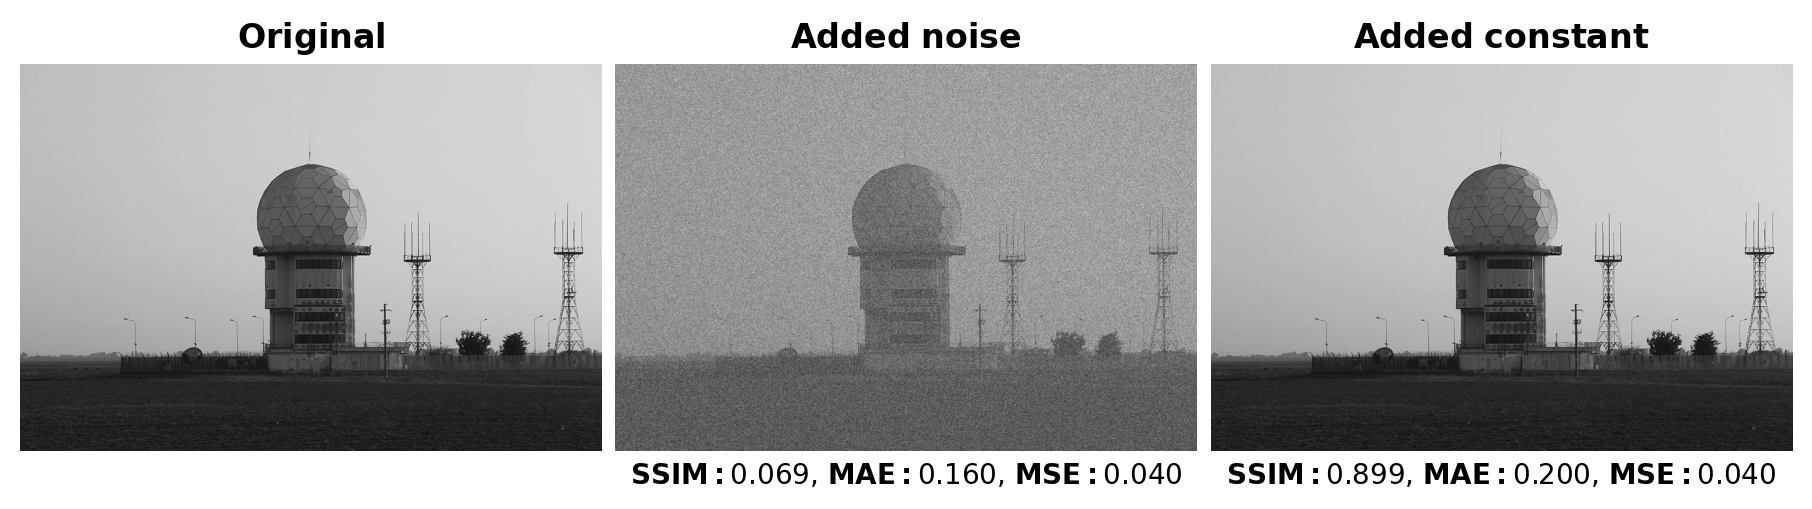
\includegraphics[width=\textwidth]{images/metrics.png}
    \caption[Differences between evaluation metrics]{\label{fig:metric}Differences between evaluation metrics. Modified images have the same \gls{MSE}, but one was created from the original by adding a random noise and the other by adding a constant. Image used for the comparison: \cite{wiki}.}
\end{figure}

\section{UNet}
\label{sec:unet}

UNet is a \gls{CNN} that was first proposed for biomedical image segmentation in the paper \cite{unet}. The architecture of this network consists of there main parts, encoder layers, bottleneck, and decoder layers. Encoders are typical convolution layers that consist of convolution stage, nonlinearity, and pooling stage\footnote{There are two conventions when it comes to the term ``layer'' in \glspl{CNN}. In one, the convolution, nonlinearity, and pooling are all called layers, and in the other layer is a term for all of them together. I will use the latter one.}. The convolution and nonlinearity stages can be repeated multiple times in one layer. A diagram showing this layer can be seen in figure \ref{fig:unet_encoder_layer}. The pooling stage reduces the resolution of the images. The convolution inside the encoder is also used for increasing the number of features.

\begin{figure}[ht]
    \centering
    \begin{subcaptionblock}[c]{\textwidth}
        \centering
        
\includegraphics[width=\textwidth]{images/unet_legend.pdf}
    \end{subcaptionblock}
    \begin{subcaptionblock}[t]{.45\textwidth}
        \centering
        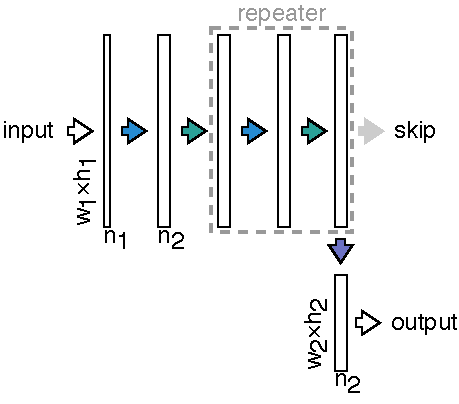
\includegraphics[height=0.8\textwidth]{images/unet_encoder.pdf}
        \caption[One layer of UNet decoder]{\label{fig:unet_encoder_layer}Encoder}
    \end{subcaptionblock}
    \begin{subcaptionblock}[t]{.45\textwidth}
        \centering
        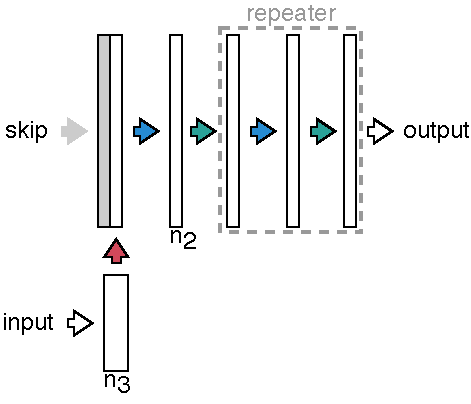
\includegraphics[height=0.8
        \textwidth]{images/unet_decoder.pdf}
        \caption[One layer of UNet decoder]{\label{fig:unet_decoder_layer}Decoder}
    \end{subcaptionblock}
    \caption[Types of layers in the UNet architecture]{\label{fig:unet_layers}Types of layers in the UNet architecture}
\end{figure}


Figure \ref{fig:unet_decoder_layer} illustrates that the decoder layer starts with upsampling the output of the previous decoder layer or bottleneck. Upsampling is done using a transposed convolution, which increases the resolution and decreases the number of features. The bottleneck is practically the same as the encoder layer but without the pooling stage at the end.

Each encoder layer in the architecture acts as a low-pass filter, suppressing details and higher spatial frequencies in the input. For the higher frequencies to be transmitted to the output, the encoder must acquire the ability to encode them in the intermediate features of the network. \cite{gunet}

The original paper \cite{unet} introduced skip-connections in order to achieve this goal. These concatenate the encoder features before the pooling stage with the upsampled features in the decoder. Concatenation is done at each ``level'' of the network, effectively bypassing the network's lower levels. These ``fast-forward'' connections, as they are sometimes called, allow for the details from the input to be transferred directly to the output without passing them through a bottleneck. Removing the need to encode the higher spatial frequencies allows, the lower levels to better capture global features. Skip connections can be seen in figures \ref{fig:unet_layers} and \ref{fig:unet_architecture}.

Similarly to the encoder, convolution with activation stages can be repeated multiple times in the decoder.

\begin{figure}[ht]
    \centering
    \begin{subcaptionblock}{\textwidth}
        \centering
        \begin{tikzpicture}[scale=.35,every node/.style={minimum size=1cm}, on grid]
            \draw[thick, fill=blue] (0,0) rectangle (1,-4);
            \draw[thick] (0.5,-4.5) to (0.5,-6);
            \draw[->, thick]  (0.5, -6) to (1.5, -6);
            \draw[thick, fill=blue] (2,-5) rectangle (4,-7);
            \draw[thick] (3,-7.5) to (3,-8.5);
            \draw[->, thick]  (3, -8.5) to (4.5, -8.5);
            \draw[thick, fill=violet] (5,-8) rectangle (9,-9);
            \draw[thick]  (9.5, -8.5) to (11, -8.5);
            \draw[->,thick] (11,-8.5) to (11,-7.5);
            \draw[thick, fill=cyan] (10,-5) rectangle (12,-7);
            \draw[thick]  (12.5, -6) to (13.5, -6);
            \draw[->,thick] (13.5,-6) to (13.5,-4.5);
            \draw[thick, fill=cyan] (13,0) rectangle (14,-4);

            \draw[->,thick,draw=gray, dashed] (1.5,-2) to (12.5,-2);
            \draw[->,thick,draw=gray, dashed] (4.5,-6) to (9.5,-6);
        \end{tikzpicture}
    \end{subcaptionblock}
    \begin{tikzpicture}[scale=0.2,every node/.style={minimum size=1cm}, on grid]
        \begin{scope}[xshift=0cm,yshift=0cm]
            \draw[draw=base03,fill=blue,thick](0,0) rectangle (1, 1);
            \node[thick,anchor=west, text centered] (p3) at (1, 0.5) {Encoder};
        \end{scope}
        \begin{scope}[xshift=12cm,yshift=0cm]
            \draw[draw=base03,fill=violet,thick](0,0) rectangle (1, 1);
            \node[thick,anchor=west, text centered] (p3) at (1, 0.5) {Bottleneck};
        \end{scope}
        \begin{scope}[xshift=24cm,yshift=0cm]
            \draw[draw=base03,fill=cyan,thick](0,0) rectangle (1, 1);
            \node[thick,anchor=west, text centered] (p3) at (1, 0.5) {Decoder};
        \end{scope}
    \end{tikzpicture}

    \caption[UNet architecture]{\label{fig:unet_architecture}UNet architecture}
\end{figure}

The architecture can be designed for tiling to take advantage of the properties of \glspl{NN} that I mentioned, particularly the equivariance to translation. Tiling means that the \gls{NN} output can be extended without increasing the network size by running the net on different ``tiles'' of the image separately to produce output in a mosaic. For this to work near the edges of the tiles, the convolutional stages cannot have padding, which means the output of the \gls{NN} will be smaller than the input. An example of this can be seen in paper \cite[fig. 2]{unet}.

\section{Bias in Neural Networkts}
\label{sec:bias}

Bias in machine learning, also sometimes called algorithm bias or AI bias, is a phenomenon that occurs when an algorithm produces systemically prejudiced results. It is separate from the bias parameter inside \glspl{NN}.

\subsection{Structural Bias}
\label{subsec:structural_bias}

\begin{figure}[ht]
    \centering
    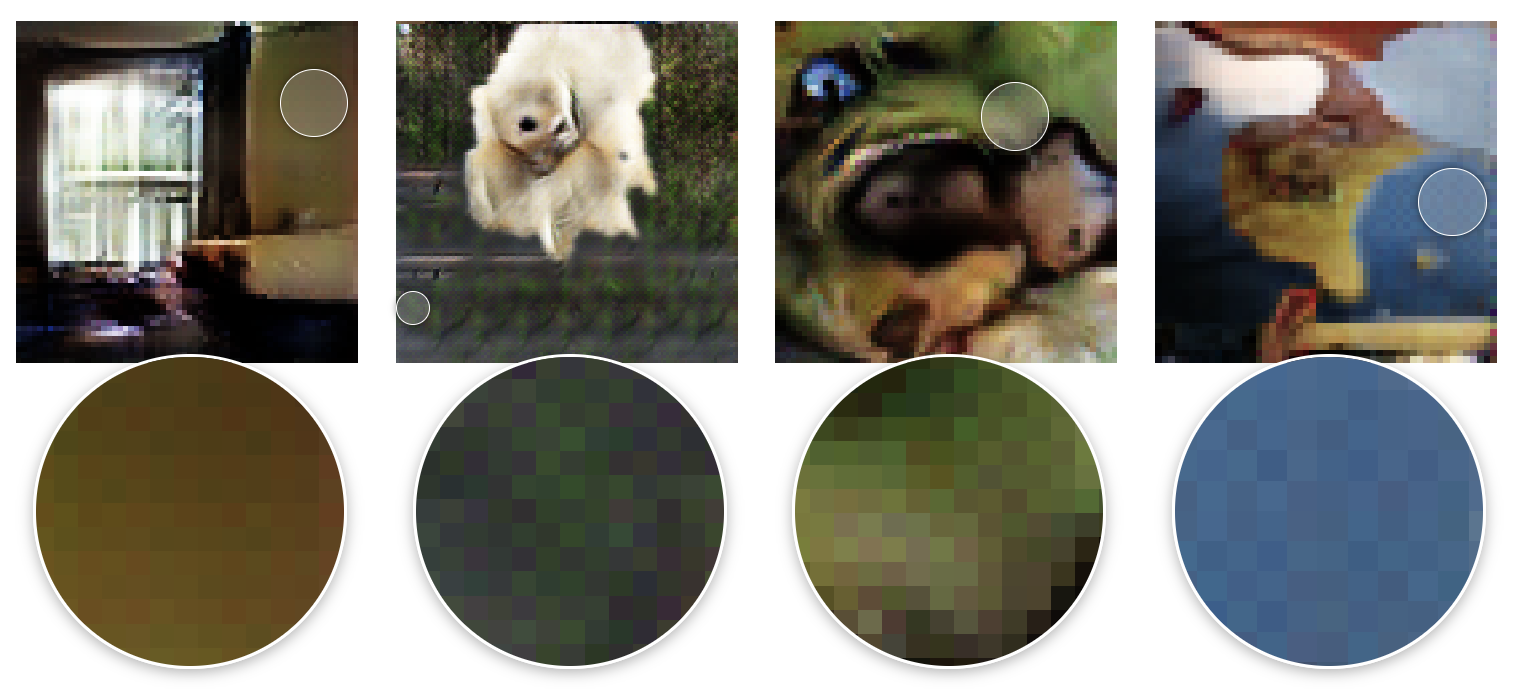
\includegraphics[width=\textwidth]{images/checkerboard_artefacts_models.png}
    \caption[Grid patterns in generative models]{\label{fig:grid_patterns_in_models}These instances show generative models that exhibit checkerboard artifacts in their outputs. The image used is sourced from \cite{deconvolutionbias}.}
\end{figure}


Many \gls{CNN} architectures employed a similar architecture to the one described in the section \ref{sec:unet} about UNet. When examining images created by these \glspl{CNN}, one may observe a distinct checkerboard pattern of irregularities, as shown in figure \ref{fig:grid_patterns_in_models}. When generating images from \glspl{NN}, the common practice is to start from lower-resolution images and gradually upscale them, which allows the \glspl{NN} to describe the rough image and then fill in some details in multiple steps. In order to achieve this, a technique for converting low-resolution images into high-resolution images is required. Transposed convolution is a commonly used method for this task, as explained in section \ref{subsec:transposed_convolution}. Layers of transposed convolutions are often found in the decoder of AutoEncoders or the generator part of \glspl{GAN}. The UNet is based on the AutoEncoder architecture and therefore uses transposed convolution.

Unfortunately, transposed convolution can easily lead to artifacts due to uneven overlap. In particular, uneven overlap in transposed convolution happens, when the kernel size is not divisible by the stride. In the section \ref{subsec:transposed_convolution}, I talked about fractional strides in transposed convolution and how they can be pictured as padding between input columns and rows. It is evident from the visualization in figure \ref{fig:transposed_convolution_artefacts} that the kernel occasionally overlaps one, two, or four inputs. This behavior forms grid-like artifacts. \glspl{CNN} generally have multiple layers with transposed convolution, so these artifacts compound on each other. \cite{deconvolutionbias}

\begin{figure}[ht]
    \centering
    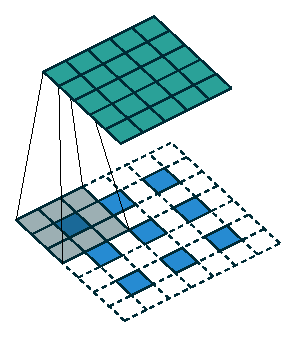
\includegraphics[width=0.24\textwidth]{images/transposed_artefacts_1.pdf}
    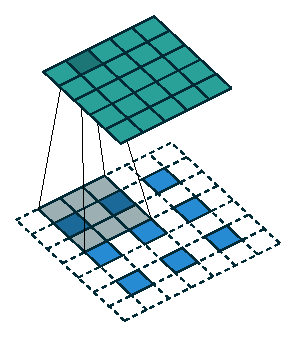
\includegraphics[width=0.24\textwidth]{images/transposed_artefacts_2.pdf}
    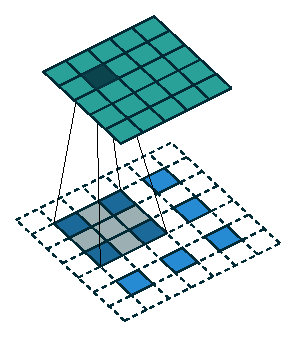
\includegraphics[width=0.24\textwidth]{images/transposed_artefacts_4.pdf}
    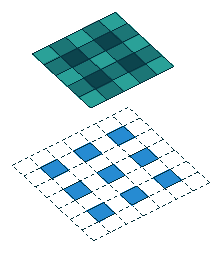
\includegraphics[width=0.24\textwidth]{images/transposed_artefacts_finished.pdf}
    \caption[Demonstration of artifact formation in transposed convolution ]{\label{fig:transposed_convolution_artefacts}
    Demonstration of artifact formation on the same transposed convolution as in figure \ref{fig:convolution_padding_strides_transposed}. \cite{convolutionguide}}
\end{figure}

The models are learning weights used in convolution and, in theory, could learn to mitigate the effects of uneven overlap. Learning to reduce these artifacts can be challenging, particularly when the convolution is done on multiple channels that impact each other. While possible, it significantly restricts the potential filters and therefore sacrifices the model's capacity. In practice, \glspl{CNN} struggle with completely avoiding these artifacts. In fact, not only do \glspl{NN} with uneven overlap not learn to avoid this, but models with even overlap often learn kernels that cause similar artifacts! While it is not their default behavior the way it is for uneven overlap, it is still very easy for transposed convolution with even overlap to cause artefacts\footnote{Even overlap happens when the kernel size is divisible by the stride.}. Completely avoiding artifacts in models with even overlap is still a significant restriction on filters, and in practice, the artifacts are still present in these models, although they seem milder.\cite{deconvolutionbias}

While many factors are at play here, the transposed convolution is a big part of the problem. It is fragile because it easily represents artifact-creating functions, even when the size is carefully chosen. At worst, creating artifacts is the default behavior of transposed convolution. In the upcoming section \ref{sec:guided_upsampling}, I will explain a method to increase the resolution of an image less susceptible to these visual abnormalities.

\subsection{Spectral Bias}
\label{subsec:spectral_bias}

Recent study \cite{spectralbias} focused on deep ReLU networks through the lens of Fourier analysis found that while \glspl{NN} can approximate arbitrary functions\footnote{See paper \cite{universalapproximators}}, they favor low-frequency ones. Therefore they exhibit a bias towards smooth functions. This phenomenon is called spectral bias. I will focus on two experiments in the study mentioned above.

In the first experiment, the researchers trained six layers deep and 256 unit wide fully-connected ReLU network on an output defined by the mapping $\lambda: [0, 1] \to \mathbb{R}$ given by

\begin{equation} \label{eq:experiment_1}
    \lambda(z) = \sum_i A_i \sin(2\pi k_i z + \varphi_i),
\end{equation}

\noindent where $\kappa = (k_1, k_2, ...)$ are the frequencies with corresponding amplitudes $\alpha = (A_1, A_2, ...)$ and phases $\phi = (\varphi_1, \varphi_2, ...)$. Network was trained to regress $\lambda$ with $\kappa = (5, 10, ..., 45, 50)$ and $N=200$ input samples spaced equally over $[0, 1]$. The spectrum of the output was monitored as training progressed. In the first setting, equal amplitudes $A_i = 1$ were set for all frequencies, and in the second setting, the amplitude gradually increased from $A_1 = 0.1$ to $A_{10} = 1$. Figure \ref{fig:spectralbias_experiment_1} shows that lower frequencies are regressed first, regardless of their amplitudes. \cite{spectralbias}

\begin{figure}[ht]
    \centering
    \begin{subcaptionblock}[t]{.475\textwidth}
        \centering
        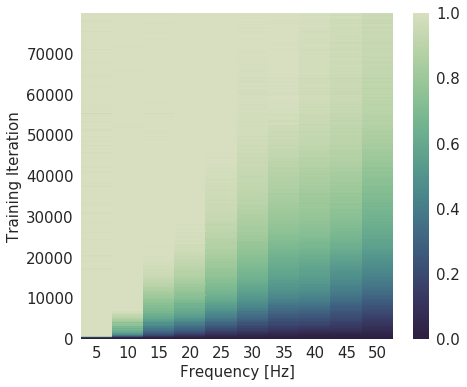
\includegraphics[height=0.9\textwidth]{images/experiment_1.png}
        \caption[Experiment showcasing spectralbias]{\label{fig:spectralbias_experiment_1}Evolution of the spectrum during training. The colors show the measured amplitude of the network spectrum at the corresponding frequency, normalized by the target amplitude at the same frequency. \cite{spectralbias}}
    \end{subcaptionblock}
    \hspace{1em}
    \begin{subcaptionblock}[t]{.475\textwidth}
        \centering
        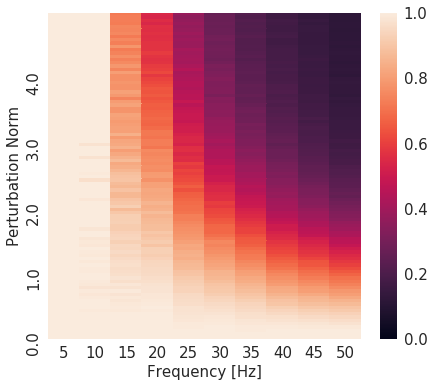
\includegraphics[height=0.9\textwidth]{images/experiment_2.png}
        \caption[Experiment showing robustness to parameter perturbation]{\label{fig:spectralbias_experiment_2}Spectrum of the model with perturbed parameters as a function of parameter perturbation. Amplitudes are normalized by the amplitudes obtained from the network without the perturbed parameters. \cite{spectralbias}}
    \end{subcaptionblock}
    \caption[Results of experiments showcasing the spectral bias]{\label{fig:spectralbias_experiments}Results of experiments from the study \cite{spectralbias} showcasing the spectral bias.}
\end{figure}

The same setup as the first experiment was used for the second experiment. Once the network had converged on certain parameters $\theta^{*}$, the authors made random perturbations $\theta = \theta^{*} + \delta \hat{\theta}$ of a specific size $\delta$, where $\hat{\theta}$ is a random unit vector in the parameter space. They evaluated the network function $f_{\theta}$ at the perturbed parameters and computed the magnitude of its discrete Fourier transform at frequencies $k_i$ to get $|\tilde{f}_{\theta}({k_i})|$. To obtain $|\tilde{f}_{\mathbb{E}\theta}({k_i})|$, which was then normalized by $|\tilde{f}_{\theta*}({k_i})|$, they averaged the results over 100 samples of $\hat{\theta}$. $|\tilde{f}_{\mathbb{E}\theta}({k_i})|$ was then averaged over the phases $\phi$ from equation \ref{eq:experiment_1},. Figure \ref{fig:spectralbias_experiment_2} displays the experiment's outcome. \cite{spectralbias}

The second experiment discovered that higher frequencies are more susceptible to changes in parameters than lower frequencies. This result suggests that precise tuning of the parameters is necessary for higher frequencies to be expressed effectively. In other words, parameters that contribute towards expressing high-frequency components occupy a small volume in the parameter space. \cite{spectralbias}

I hypothesize that the use of transposed convolution negatively impacts the learning of higher frequencies. It may not be possible to fine-tune the parameters required for capturing higher frequencies due to the limitations on filters in transposed convolution, as discussed in section \ref{subsec:transposed_convolution}. Increasing the likelihood of the model learning higher frequencies can be achieved by removing the structural biases that arise from upscaling using transposed convolution. In the following section \ref{sec:guided_upsampling}, I will focus on one upsampling method that aims to accomplish this by replacing the transposed convolution with guided upsampling.

\section{GUNet: Guided UNet}
\label{sec:guided_upsampling}

Transposed convolution in the decoder layers of the UNet architecture can cause checkerboard artifacts, as mentioned in section \ref{subsec:structural_bias}. Other non-learned upsampling methods can cause blurring since they are based on pre-defined interpolation.

Several methods that attempt to alleviate these upsampling artifacts have been proposed. A resize convolution technique is introduced in the research paper \cite{deconvolutionbias}. This method utilizes a technique that separates upsampling from convolution to ensure more precise feature computation. Before the convolution process, the image is resized using either nearest-neighbor or bilinear interpolation. Other methods try to reduce the checkerboard artifacts by correlating the kernel weights in transposed convolution. An example of such a method can be found in the paper \cite{aitken2017checkerboard}, which proposes a specialized initialization scheme for transposed convolutional layers that correlates the kernel weights at initialization. These methods generally eliminate the artifacts, but they fail to use the high-frequency details from the encoder efficiently and are trying to extract the information in the decoder. Non-learned methods are also prone to blurring. Furthermore, it should be noted that utilizing learned upsampling through transposed convolutions, even when the kernel weights are correlated, does not assure the avoidance of minima that produce artifacts during optimization, as previously discussed in section \ref{subsec:structural_bias}. \cite{gunet}

This section describes the \gls{GUNet} architecture proposed in the paper \cite{gunet}.

\subsection{Guided Image Filtering}
\label{subsec:guided_image_filtering}

\gls{GIF} is an edge-preserving smoothing filter. Its main advantage over bilateral filters is the computational complexity. The output image of the \gls{GIF} is consistent with the gradient direction of the guidance image, which prevents gradient reversal prominent in the bilateral filters.

\gls{GIF} works by assuming that there is a local linear model between the guidance $I$ and the filtering output $q$. The following definition of the filter is taken directly from the paper \cite{gif}, in which the filter was proposed.

\vspace{1em}
{\itshape
\noindent We assume that $q$ is a linear transform of $I$ in a window $\omega_{k}$ centered at the pixel $k$:

\begin{equation} \label{eq:linear_model}
    q_{i}=a_{k}I_{i}+b_{k}, \forall i \in \omega_{k},
\end{equation}

\noindent where $a_k$ and $b_k$ are some linear coefficients assumed to be constant in $\omega_{k}$. We use a square window of a radius $r$.

\noindent To determine the linear coefficients $a_k$ and $b_k$, we need constraints from the filtering input $p$. We model the output $q$ as the input $p$ subtracting some unwanted components $n$ like noise/textures:

\begin{equation}
    q_{i}=p_{i}-n_{i}.
\end{equation}

\noindent We seek a solution that minimizes the difference between $q$ and $p$ while maintaining the linear model in equation \ref{eq:linear_model}. Specifically, we minimize the following cost function in the window $\omega_{k}$:

\begin{equation} \label{eq:linear_ridge_regression}
    E(a_{k}, b_{k})=\sum_{i \in \omega_{k}}\big(\big(a_{k}I_{i}+b_{k}-p_{i}\big)^{2}+\epsilon a_{k}^{2}\big).
\end{equation}

\noindent Here, $\epsilon$ is a regularization parameter penalizing large $a_k$. Equation \ref{eq:linear_ridge_regression} is the linear ridge regression model, and its solution is given by

\begin{align} \label{eq:gif_coefficient}
    a_{k}={{1\over \vert \omega \vert } \sum_{i\in \omega_{k}}I_{i}p_{i}-\mu_{k}\bar{p}_{k}\over \sigma_{k}^{2}+\epsilon }, && b_{k}=\bar{p}_{k}-a_{k}\mu_{k}.
\end{align}

\noindent Here, $\mu_{k}$ and $\sigma_{k}^{2}$ are the mean and variance of $I$ in $\omega_{k}$, $\vert \omega \vert$ is the number of pixels in $\omega_{k}$, and $\bar{p}_{k} = \frac{1}{ \vert \omega \vert } \sum_{i\in \omega_{k}}p_{i}$ is the mean of $p$ in $\omega_{k}$. Having obtained the linear coefficients $a_k$ and $b_k$, we can compute the filtering output $q_i$ by equation \ref{eq:linear_model}.

\noindent However, a pixel $i$ is involved in all the overlapping windows $\omega_{k}$ that covers $i$, so the value of $q_i$ in equation \ref{eq:linear_model} is not identical when it is computed in different windows. A simple strategy is to average all the possible values of $q_i$. So after computing $a_k$ and $b_k$ for all windows $\omega_{k}$ in the image, we compute the filtering output by

\begin{equation} \label{eq:filtering_output}
    q_{i}={1\over \vert \omega \vert } \sum_{k \vert i \in \omega_{k}}(a_{k}I_{i}+b_{k}).
\end{equation}

\noindent Noticing that $\sum_{k \vert i \in \omega_{k}}a_{k}= \sum_{k \in \omega_{i}}a_{k}$ due to the symmetry of the box window, we rewrite equation \ref{eq:filtering_output} by

\begin{equation} \label{eq:gif}
    q_{i}=\bar{a}_{i}I_{i}+\bar{b}_{i},
\end{equation}

\noindent where $\bar{a}_{i} = {1\over \vert \omega \vert} \sum_{k \in \omega_i}a_k$ and $\bar{b}_{i} = {1\over \vert \omega \vert} \sum_{k \in \omega_i}b_k$ are the average coefficients of all windows overlapping $i$.

}
\vspace{1em}

The definition of the guided filter is provided by equations \ref{eq:gif_coefficient} and \ref{eq:gif}. Local linear model in equation \ref{eq:linear_model} ensures that $q$ has an edge only if $I$ has an edge because the gradient of $q$ is just scaled gradient of $I$ ($\nabla q=a \nabla I$). After the modifications in equation \ref{eq:gif}, this no longer holds true because the linear coefficients $\bar{a}_i$ and $\bar{b}_i$ vary spatially. Nevertheless, as $\bar{a}_i$ and $\bar{b}_i$ are the output of a mean filter, their gradients can be expected to be much smaller than that of $I$ near strong edges. In this situation, we can still have $\nabla q\approx \bar a \nabla I$, meaning that abrupt intensity changes in $I$ can be mostly preserved in $q$. \cite{gif}

The algorithm constructed from this definition runs in $O(N)$ and can be improved to $O(N/s^2)$, where $s$ is a subsampling ratio. Improve\-ment is achie\-ved using a \gls{FGF} described in paper \cite{fastguided}. In various applications, this leads to a speedup of more than ten times with almost no visible degradation. A pseudocode to both algorithms can be found in the appendix \ref{ax:gif}.

\subsection{Guided Upsampling}
\label{subsec:guided_upsampling}

Due to computational and memory costs, it is beneficial to downsample large images when performing image analysis and enhancement tasks such as tone mapping, colorization, stereo depth rendition, and photomontage. The result is then obtained by upsampling the solution computed on the smaller images. This upsampling does not consider the additional information in the original high-resolution image. Images upsampled by convolving the low-resolution image with an interpolation kernel typically also suffer from a blurring of sharp edges because of the smoothness inherent in the linear interpolation filters. A \gls{JBU} operation was proposed in the paper \cite{bilateral}, which leverages this information and produces outstanding full-resolution results from stereo depth rendition, image colorization, adaptive tone mapping, and graph-cut based image composition computed at very low resolutions.

Just like \gls{JBU}, \gls{GIF} can be utilized for upsampling by using an initial image as a basis for the operation. The algorithm differs from the one in section \ref{subsec:guided_image_filtering} because we now have a guidance image at a different scale than the filtering input. In this case, we compute the linear coefficient $a$ and $b$ in using the equation \ref{eq:gif_coefficient} at the coarse scale, bilinearly upsample them to the fine-scale (replacing the mean filter on $a$ and $b$) and compute the output by $q = aI + b$ at this scale. The result of \gls{GU} is visually comparable to the \gls{JBU}. \cite{gif}

\gls{GIF} provides a better performance than the bilateral filter used in \gls{JBU}, as I previously mentioned. The upsampling adjustments can also be made on \gls{FGF} for an even faster algorithm.

\subsection{Guided UNet Architecture}
\label{subsec:review_gunet_architecture}

\gls{GIF} can be incomported in the UNet architecture discussed in section \ref{sec:unet}. Using \gls{GIF}, we can benefit from the filter's edge-preserving nature and use the higher-level features from the encoder as guidance in the upsampling. UNet takes advantage of skip connections and combines them with features that pass through the bottleneck by concatenating them and combining them with convolution. \gls{GUNet} architecture proposed in paper \cite{gunet} replaces this with \gls{GU}.

In contrast to the UNet method, two skip connections are used in the upsampling process, which involves two levels of resolution: high and low. We can upscale the low-resolution feature by utilizing information from features in the skip connections of encoders from both levels.

Both of these features are used as guides in the filter. Let's call them $I^{\texttt{hr}}$ and $I^{\texttt{lr}}$. Input to the filter is an output of the previous decoder or bottleneck layer\footnote{When upsampling the bottleneck features in the first decoder, there is no skip-connection of lower-resolution we can use. One effective way to address this issue is to utilize the bottleneck as a lower resolution guide \textit{and} as an input for the filter.}. The illustrations of how this works can be found in figures \ref{fig:gunet_decoder} and \ref{fig:gunet_architecture}.

The operations of the \gls{GU} are modified to accommodate two guides. According to the paper \cite{gunet}, lower-resolution guide $I^{\texttt{lr}}$ and input $p$ are used to compute $\bar a_k^{\texttt{lr}}$ and $\bar b_k^{\texttt{lr}}$ on the lower resolution. The coefficients are then upsampled back to the higher resolution to form $\bar a_k^{\texttt{hr}}$ and $\bar b_k^{\texttt{hr}}$, using bilinear upsampling. The coefficients are then applied on the higher resolution guidance feature $I^{\texttt{hr}}$ to compute the final filtered decoder feature:

\begin{equation}\label{eq:guided_upsampling}
    q_i = \bar a_i^{\texttt{hr}}I^{\texttt{hr}} +\bar b_i^{\texttt{hr}}.
\end{equation}

The dotted arrows in figure \ref{fig:gunet_decoder} represent the abovementioned operations. Some readers might have noticed the discrepancy in the channel counts of lower coefficients ($\bar a_k^{\texttt{lr}}$, $\bar b_k^{\texttt{lr}}$) and higher coefficients ($\bar a_k^{\texttt{hr}}$, $\bar b_k^{\texttt{hr}}$). The authors of the paper state that the upsampling is done on each channel separately, but this poses a challenge, which I will discuss in the section \ref{subsed:channel_discrepancy}. One solution might be to use convolution to decrease channel counts of low-resolution coefficients.

\begin{figure}[h]
    \centering
    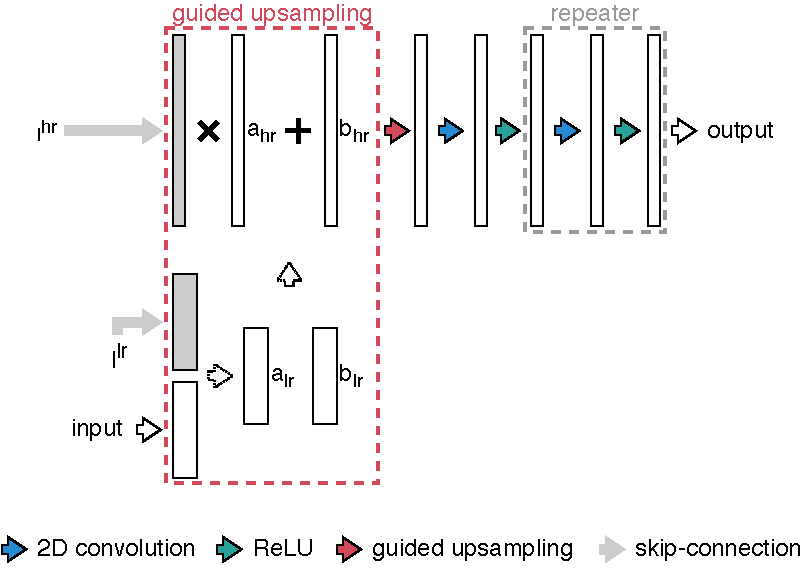
\includegraphics[width=0.8\textwidth]{images/gunet_decoder.pdf}
    \caption[Decoder layer in the GUNet architecture]{\label{fig:gunet_decoder}Decoder layer in the GUNet architecture}
\end{figure}

Guided feature upsampling combines the encoder and decoder features of the architecture and aims to guide its features at each upsampling stage in the output to be structurally similar to the corresponding feature set of the input features in the encoder. It is worth pointing out that \gls{GUNet} results in fewer parameters than UNets with transposed convolutions since the upsampling is parameter-free\footnote{Even if we use convolution to decrease the channel counts of the low-resolution coefficients $\bar a_k^{\texttt{lr}}$ and $\bar b_k^{\texttt{lr}}$} and the concatenation layer is avoided. The paper \cite{gunet} later investigates the effects of the structural biases of \glspl{CNN} on network outputs. The improvement attained by \gls{GUNet} was evident in the Fourier domain. The effectiveness of this approach was demonstrated in the inverse tone mapping and colorization of grayscale images. State-of-the-art performance was achieved in the inverse tone mapping application. In colorization, \gls{GUNet} exhibited benefits compared to alternative UNet architectures. \cite{gunet}

My goal is to apply this architecture to weather nowcasting and compare it with the traditional UNet both in the Fourier domain and using traditional metrics such as \gls{SSIM}, \gls{MAE}, and \gls{MSE}.

\begin{figure}[ht]
    \centering
    \begin{subcaptionblock}{\textwidth}
        \centering
        \begin{tikzpicture}[scale=.4,every node/.style={minimum size=1cm}, on grid]
            \draw[thick, fill=blue] (0,0) rectangle (1,-4);
            \draw[thick] (0.5,-4.5) to (0.5,-6);
            \draw[->, thick]  (0.5, -6) to (1.5, -6);
            \draw[thick, fill=blue] (2,-5) rectangle (4,-7);
            \draw[thick] (3,-7.5) to (3,-8.5);
            \draw[->, thick]  (3, -8.5) to (4.5, -8.5);
            \draw[thick, fill=violet] (5,-8) rectangle (9,-9);
            \draw[thick]  (9.5, -8.5) to (15, -8.5);
            \draw[->,thick] (15,-8.5) to (15,-7.5);
            \draw[thick, fill=cyan] (14,-5) rectangle (16,-7);
            \draw[thick]  (16.5, -6) to (17.5, -6);
            \draw[->,thick] (17.5,-6) to (17.5,-4.5);
            \draw[thick, fill=cyan] (17,0) rectangle (18,-4);

            \draw[->,thick,draw=gray, dashed] (1.5,-1.5) to (16.5,-1.5);
            \draw[->,thick,draw=gray, dashed] (5.5,-2.5) to (16.5,-2.5);
            \draw[thick,draw=gray, dashed] (5.5,-2.5) to (5.5,-5.5);

            \draw[->,thick,draw=gray, dashed] (4.5,-5.5) to (13.5,-5.5);
            \draw[->,thick,draw=gray, dashed] (10.5,-6.5) to (13.5,-6.5);
            \draw[thick,draw=gray, dashed] (10.5,-6.5) to (10.5,-8.5);
        \end{tikzpicture}
    \end{subcaptionblock}
    \begin{tikzpicture}[scale=0.2,every node/.style={minimum size=1cm}, on grid]
        \begin{scope}[xshift=0cm,yshift=0cm]
            \draw[draw=base03,fill=blue,thick](0,0) rectangle (1, 1);
            \node[thick,anchor=west, text centered] (p3) at (1, 0.5) {Encoder};
        \end{scope}
        \begin{scope}[xshift=12cm,yshift=0cm]
            \draw[draw=base03,fill=violet,thick](0,0) rectangle (1, 1);
            \node[thick,anchor=west, text centered] (p3) at (1, 0.5) {Bottleneck};
        \end{scope}
        \begin{scope}[xshift=24cm,yshift=0cm]
            \draw[draw=base03,fill=cyan,thick](0,0) rectangle (1, 1);
            \node[thick,anchor=west, text centered] (p3) at (1, 0.5) {Decoder};
        \end{scope}
    \end{tikzpicture}

    \caption[GUNet architecture]{\label{fig:gunet_architecture}GUNet architecture}
\end{figure}
\chapter{Methodology}
\label{chap:methodology}


\section{Dataset}
\label{sec:dataset_description}

I used a collection of radar images to train and evaluate the models. These radar images were composites from a heterogeneous network of operational weather radars created by \gls{OPERA} \cite{weatherradar}. In October 2013, the network consisted of 202 operational radars, of which 184 had Doppler capability and 48 were dual-polarization radars. Most radars operate at the C band (168 sites). However, several S-band radars are installed in the south of Europe (33 sites)\footnote{For more information about different radars used in weather nowcasting, refer to section \ref{subsec:radars}}.

\begin{figure}[ht]
    \centering
    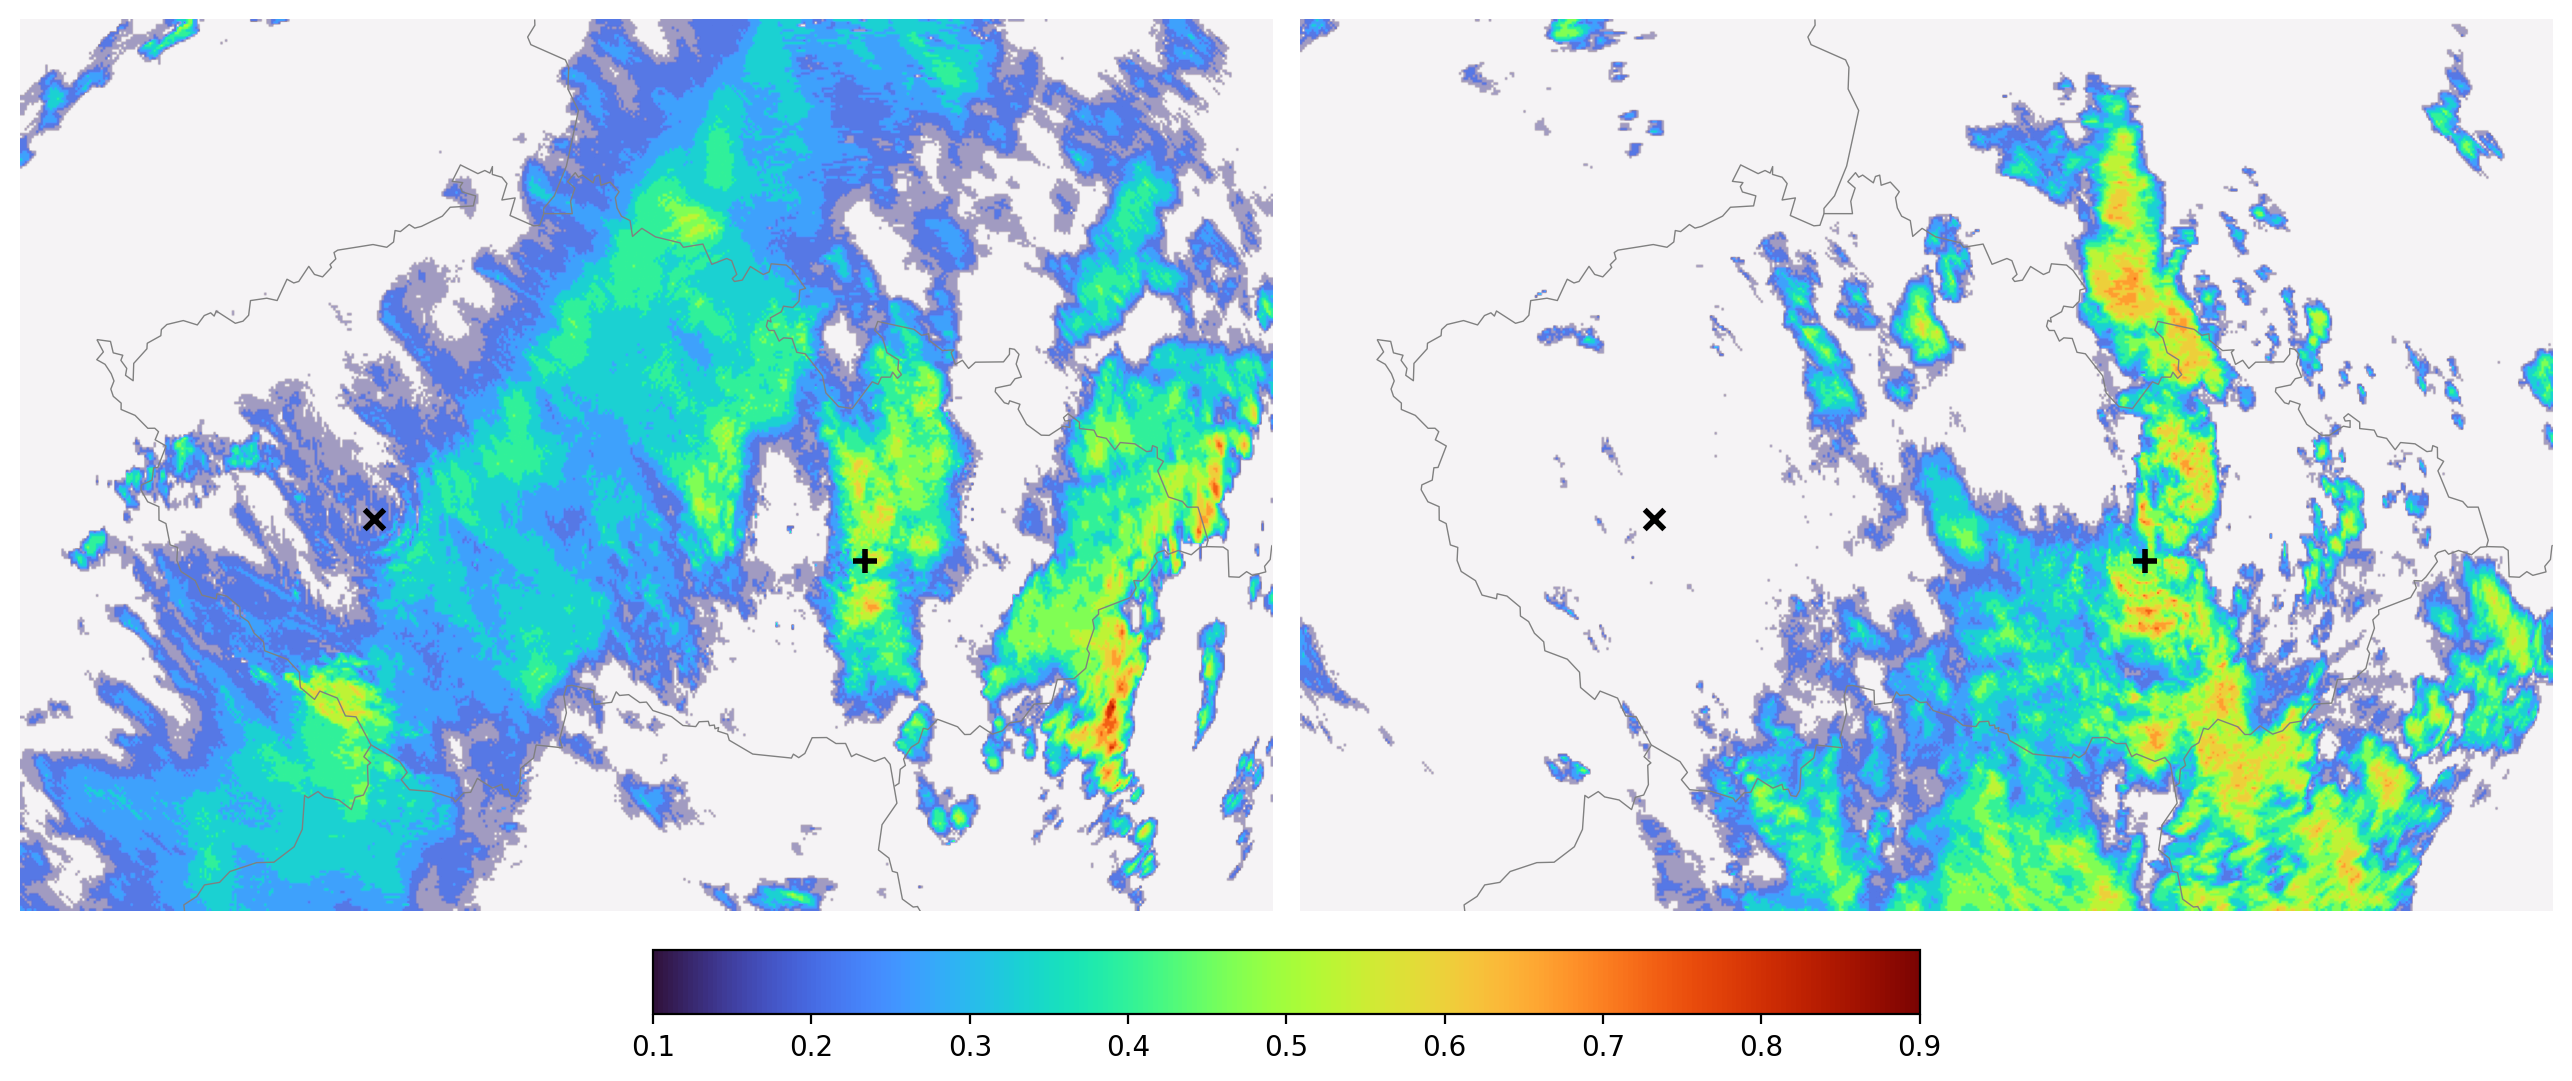
\includegraphics[width=\textwidth]{images/radar_image_with_map.png}
    \caption[Example of radar images from the dataset]{\label{fig:radar_image_with_map}Example of images from the dataset after preprocessing. Values smaller than the lower bound of the color bar are transparent, and those higher than the upper bound are displayed as if they were equal to it. Positions of Czech radars are marked with symbols × (Brdy-Praha) and + (Skalky).}
\end{figure}

The \gls{OPERA} Radar Data Center (Odyssey) has been operational since 2011. Polar volume data are collected from 134 radar sites in 21 countries, and continental scale mosaic products (surface rain rate, rainfall accumulation, and maximum reflectivity) are generated in real-time. These mosaic products are generated on a Cartesian grid covering Europe (3800×4400 $\text{km}^2$). \cite{weatherradar}

The images I used cover the area above the Czech Republic, as illustrated in figure \ref{fig:radar_image_with_map}. The resolution of images is 544×352 pixels, where one pixel represents an area of 1 $\text{km}^2$. Images are generated every 10 minutes, but some may be missing. Absent images were taken into account when creating network inputs and targets. The dataset covers the period from October 23, 2015, to July 21, 2020.

\subsection{Data Preprocessing and Augmentation}
\label{sec:data_preprocessing}

The radar data from \gls{OPERA} was already cleaned using a combination of anomaly removal and hit-accumulation clutter filtering, which was done by the anomaly-removal module\footnote{Some anomalies are still visible in the figure \ref{fig:radar_image_with_map} in the form of circles around the radars.}.

In the mosaic, each pixel comprises of data from different multiple radars and elevations. The highest value from all the available heights and radars is chosen for each pixel. The dataset's images have a maximum reflectivity captured in 16 values ranging from 0 to 60 dBZ. These values are then mapped to a range of 0 to 255. I utilized min-max normalization to ensure all values ranged from 0 to 1. I then cropped a rectangle of 512×256 pixels from the images, preventing pooling problems\footnote{Pooling is used in both models with 2×2 stride and 2×2 kernel, which halves the feature resolution in both axes. This pooling can be performed without padding or dropping values when the images have sides equal to powers of two. See section \ref{subsec:convolution} about convolution and section \ref{subsec:pooling} about pooling.}.

\begin{figure}[ht]
    \centering
    \begin{subcaptionblock}[t]{.45\textwidth}
        \centering
        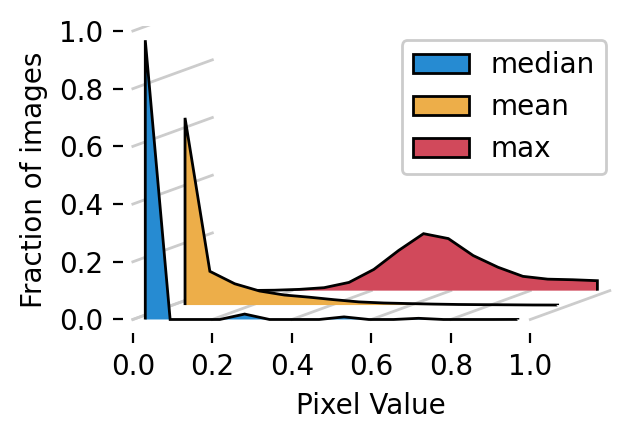
\includegraphics[width=\textwidth]{images/hist_dataset.png}
        \caption[Distribution maximum, median, and mean values for each image in the dataset]{\label{fig:hist_dataset}Distribution of maximum, median, and mean values for each image in the dataset.}
    \end{subcaptionblock}
    \hspace{1em}
    \begin{subcaptionblock}[t]{.45\textwidth}
        \centering
        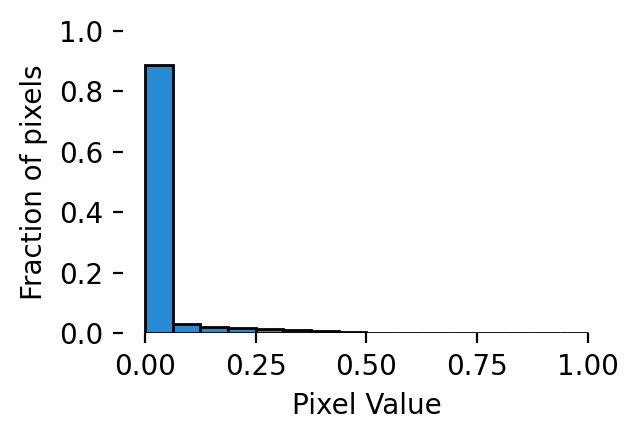
\includegraphics[width=\textwidth]{images/hist_dataset_pixels.png}
        \caption[Distribution of pixel values in the dataset]{Distribution of individual pixel values in the dataset.}
    \end{subcaptionblock}
    \caption[Distribution of radar echo intensities in the dataset]{Distribution of radar echo intensities in the dataset.}
\end{figure}

I did not exclude any images from the data. In hindsight, it may have been a mistake not to do this because the dataset includes numerous almost empty images, as illustrated in figure \ref{fig:hist_dataset}.

\subsection{Creating Data Points}
\label{sec:data_points}

Both models were trained on a sequence of consecutive images spaced by parameter \texttt{stride}\footnote{Parameter \texttt{stride} is in minutes.}. The dataset was split into chunks, each containing \texttt{chunk\_size} of images from the sequence. Data points were generated by setting an \texttt{input\_length}, and \texttt{target\_length}.

A sliding window of length $\texttt{input\_length} + \texttt{target\_length}$ is then moved along the images in one chunk. Each position of the sliding window represents one data point for the models. The corresponding data point will not be created if the dataset has a missing image in data points inputs or outputs.

The dataset is split by randomly assigning generated chunks to some of the datasets. Two consecutive chunks have no overlap, which is essential for creating training, validation, and testing datasets. The probability of assigning a chunk to one of the datasets is given by parameters \texttt{test\_frac} and \texttt{val\_frac} representing fractions of the dataset which will be used for testing and validation respectively\footnote{The probability that these datasets will contain the same number of images is small, because, aside from the randomness, the chunks do not contain the same number of data points due to the missing images.}. Data points in assigning chunks are then concatenated to create the datasets. The random assigning can be seeded by setting the \texttt{seed} parameter. This way, the same datasets are generated each time.

\begin{figure}[ht]
    \centering
    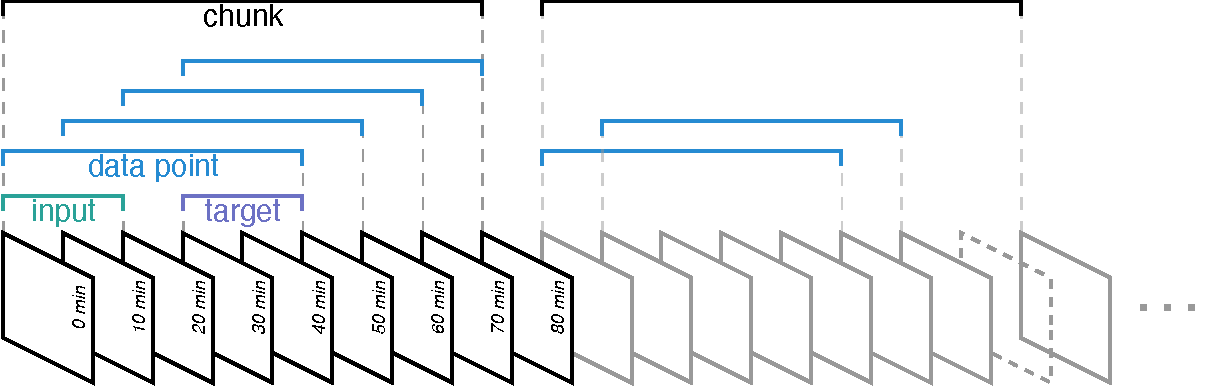
\includegraphics[width=\textwidth]{images/dataset.pdf}
    \caption[Process of generating data points from the dataset]{\label{fig:data_points}Generating data points from the dataset in chunks. Datapoint is added to the chunk only if it has no missing images in the input or target images. There is no overlap of data points between different chunks.}
\end{figure}

Adjusting the \texttt{chunk\_size}\footnote{Parameter \texttt{chunk\_size} needs to be $\geq$ than $\texttt{input\_length} + \texttt{target\_length}$.} changes the number of data points overall as smaller chunks skip more images to maintain no overlap between the chunks. I chose these values for the parameters:

\begin{align*}
    &\texttt{stride} = 10,&  &\texttt{test\_frac} = 0.1,& &\texttt{val\_frac} = 0.1,& &\texttt{seed} = 42, \\
    &\texttt{chunk\_size} = 100,& &\texttt{input\_length} = 8,& &\texttt{target\_length} = 8.&    &
\end{align*}

\noindent This resulted in training, validation, and testing datasets with 168110, 21108, and 20957 data points, respectively. The whole process is depicted in figure \ref{fig:data_points}.

\section{UNet}
\label{sec:standard_unet}

I chose similar architecture as in the original paper \cite{unet}. The network has five ``levels'', meaning five pooling and transposed convolution layers exist. The encoder layer consists of a convolution block and max pooling. As mentioned earlier, max pooling is done with 2×2 strides and 2×2 kernel.

Convolution block is a sequence of 2D convolution followed by Batch normalization, ReLU, and Dropout. The convolution block can be repeated multiple times. I chose to do three repetitions. All 2D convolutions in the block are executed with 1×1 stride and 3×3 kernel and 1×1 padding\footnote{In practice, it would be better to use no padding and therefore have smaller output than input. Doing it this way guarantees the same network output near edges when tiling larger surfaces. See \cite[fig. 2]{unet}}.

\textit{Batch normalization} is a technique used in deep learning to improve the training process of artificial neural networks\footnote{See paper \cite{batchnorm}.}. I used it as it has been shown to improve training speed, enable the use of higher learning rates, and often lead to better generalization performance. \textit{Dropout} is a regularization technique used in neural networks to prevent overfitting and improve generalization\footnote{See paper \cite{dropout}}. During the training process, Dropout randomly ``drops out"\footnote{I. e. temporarily removes or sets to 0.} a proportion of the neurons in a given layer at each training step. The dropped-out neurons do not contribute to that training iteration's forward or backward pass. A hyperparameter called the \texttt{dropout\_rate} can set the probability of a neuron being dropped.

The number of output channels from the convolution block can be adjusted by setting different values of parameters \texttt{in\_channels} and \texttt{out\_channels}. The first convolution in the block changes the number of feature maps as described in the section \ref{subsec:convolution} and figure \ref{fig:convolution_kernel_collection}. In the encoder, the number of features is doubled each time.

The decoder layer begins with a transposed convolution. The output of this operation is then combined with a feature from the skip connection. Convolution block follows, but this time the number of features is halved. The transposed convolution also halves the number of features. It has a 2×2 stride and variable kernel size, which is given by parameter \texttt{kernel\_size} when the network is initialized. I will examine how this parameter's best value was found later in the section \ref{subsec:hyperparameters}. Padding in transposed convolution must be adjusted based on the kernel size to $\lfloor (k - 2) / 2 \rfloor$.

Finally, preventing some artifacts which may appear from the transposed convolution is achieved by 2D convolution with 1×1 stride and 1×1 kernel. Moreover, I added a sigmoid activation as the network's last layer to make the network outputs in the correct range. Figure \ref{fig:my_unet_diagram} shows a diagram of the implementation. The network used for eventual training had 11 713 080 parameters, all trainable. The size of the weights is 44.68 MB.

\begin{figure}[ht]
    \centering
    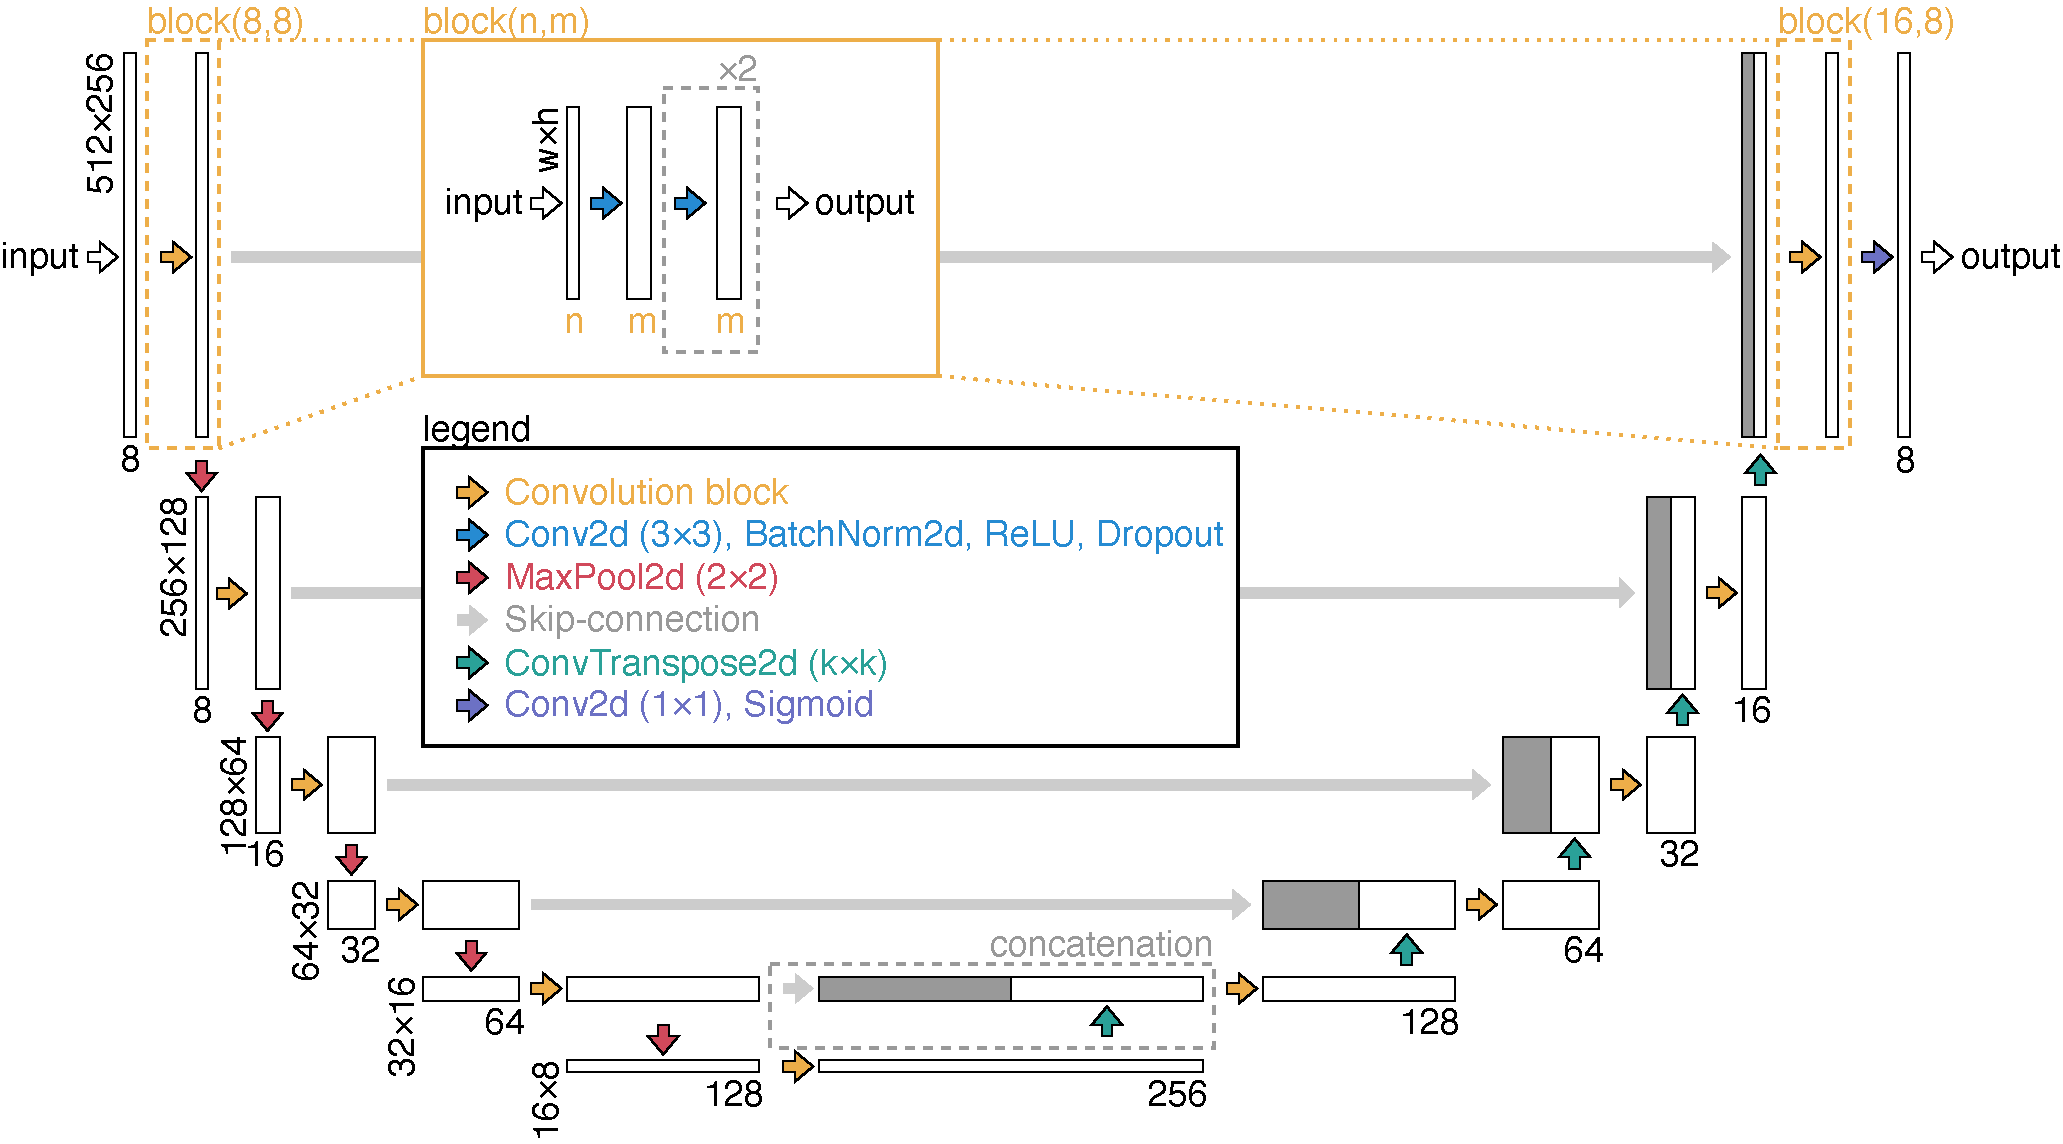
\includegraphics[width=\textwidth]{images/my_unet_diagram.pdf}
    \caption[UNet implementation diagram]{\label{fig:my_unet_diagram}UNet implementation diagram.}
\end{figure}

\section{GUNet}
\label{sec:methodology_gunet}

My implementation of the \gls{GUNet} architecture is inspired by the one in the paper \cite{gunet}. It is similar to the UNet, as portrayed in figure \ref{fig:my_gunet_diagram}. The convolution block, which follows the same structure as in the UNet architecture, uses 1×1 stride, 3×3 kernel, and 1×1 padding for all 2D convolutions. The network's final layers utilize 2D convolution with a 1×1 stride and 1×1 kernel, along with sigmoid activation.

Upsampling modules inside the decoder are replaced by \gls{GU}\footnote{Workings of \gls{GU} are described in section \ref{subsec:guided_upsampling}}. The \gls{GIF} in \gls{GU} has two parameters\footnote{See section \ref{subsec:guided_image_filtering}}: $\epsilon$, a regularization parameter penalizing large $a_k$ and $r$ which is a radius defining $\omega_{k}$. The value of these parameters was found by hyperparameter search, which I explore in the section \ref{subsec:hyperparameters}. Using \gls{GIF} instead of transposed convolution lowered the number of trainable parameters to 10 578 728, which take up 40.35 MB.

\begin{figure}[ht]
    \centering
    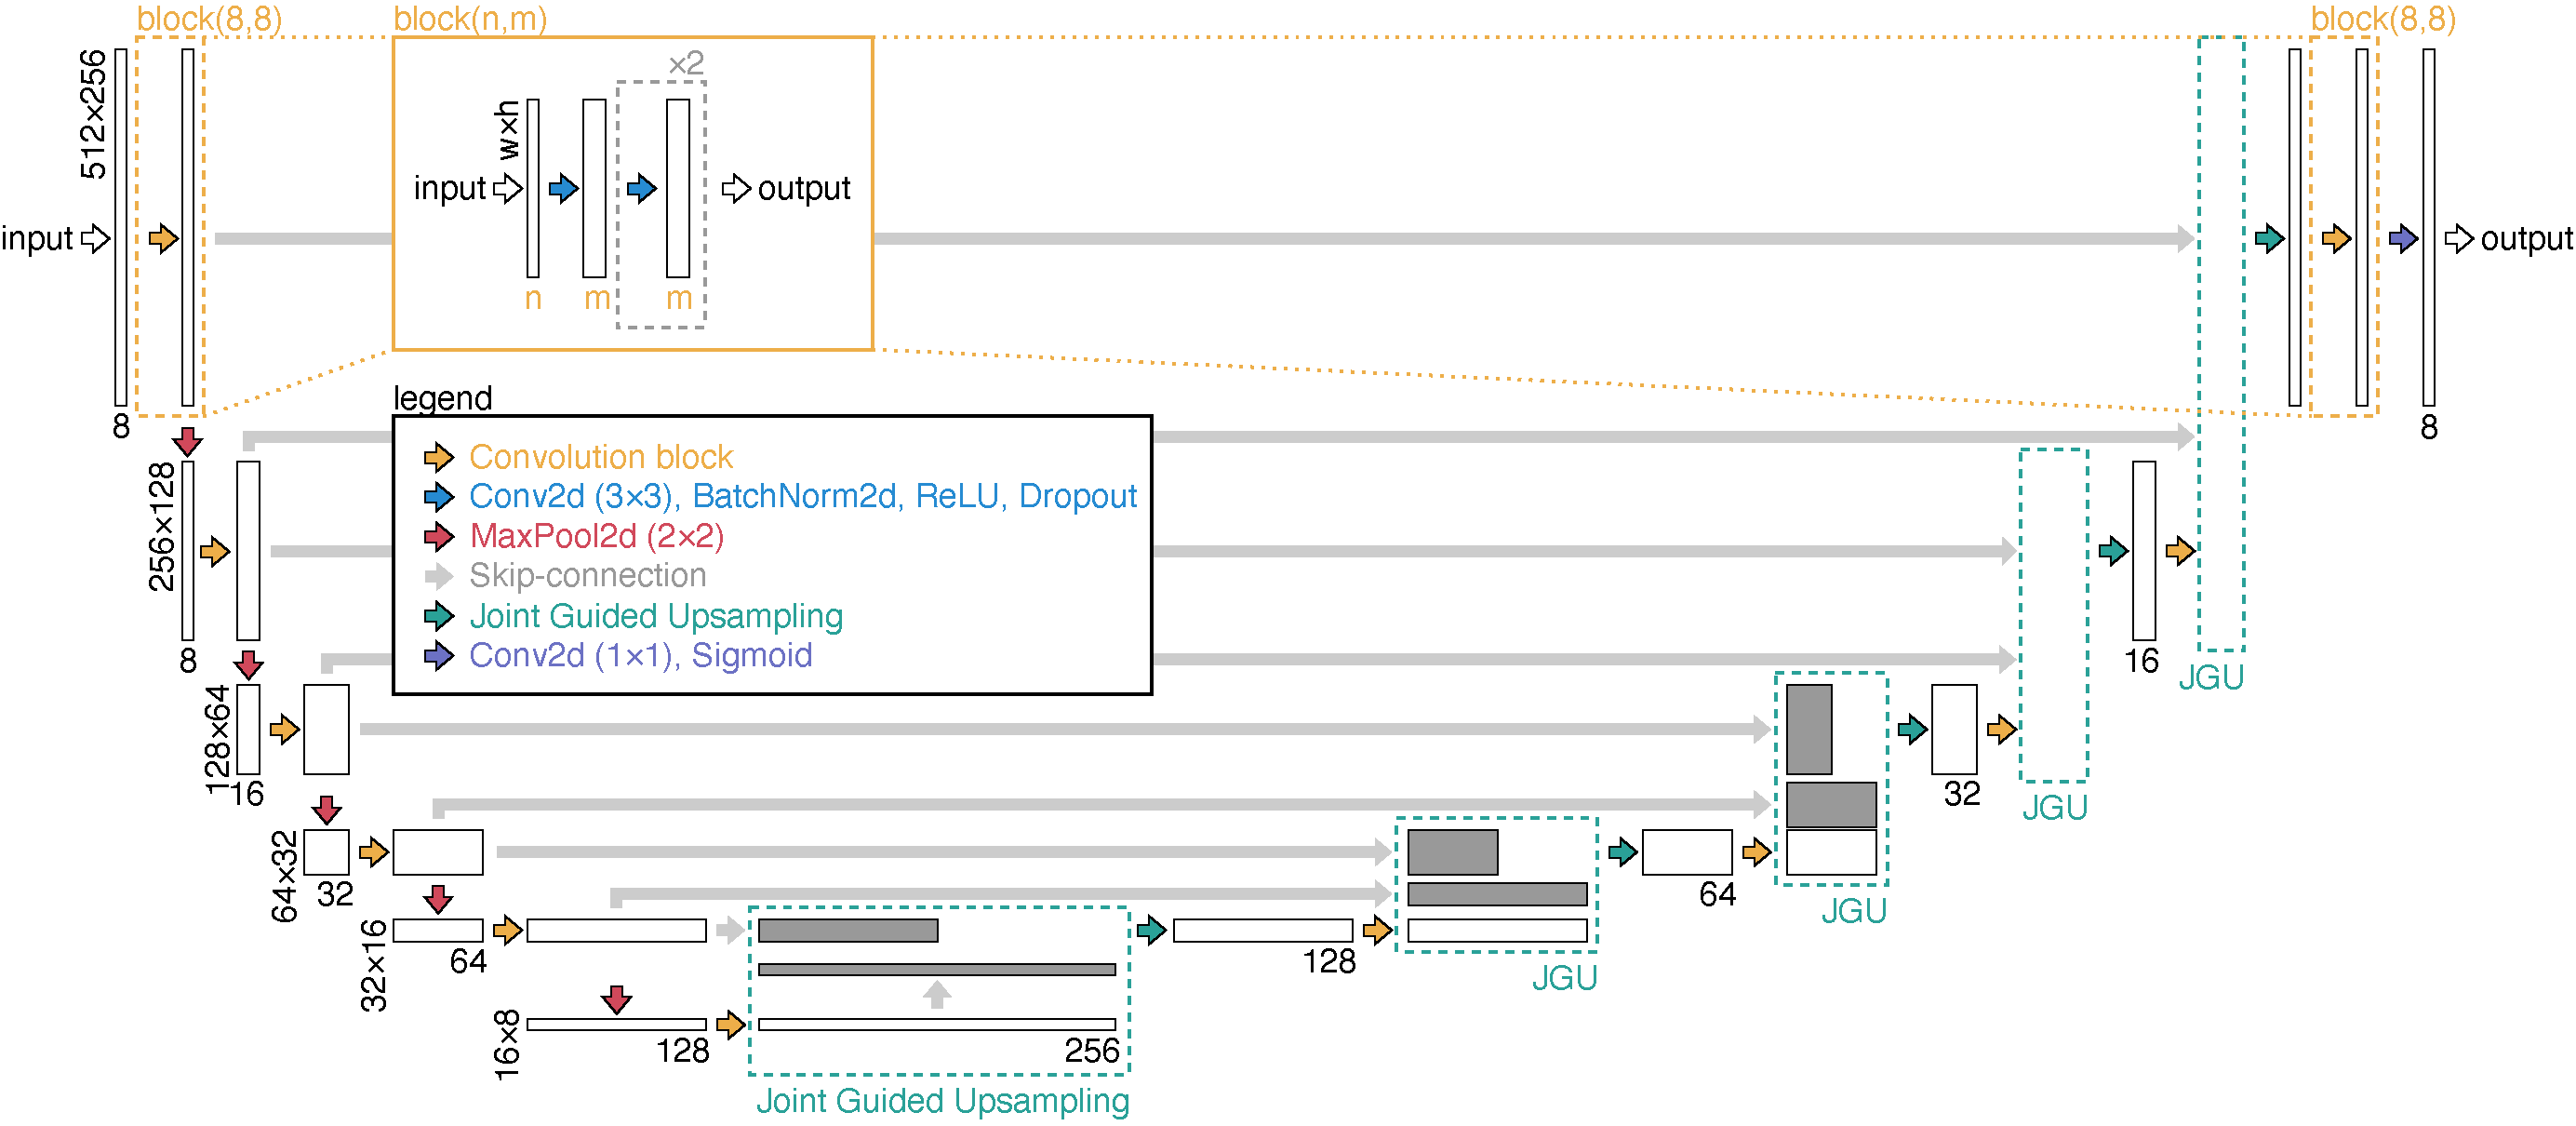
\includegraphics[width=\textwidth]{images/my_gunet_diagram.pdf}
    \caption[GUNet implementation diagram]{\label{fig:my_gunet_diagram}GUNet implementation diagram.}
\end{figure}

\subsection{Feature Channel Count Discrepancy}
\label{subsed:channel_discrepancy}

The \gls{GU} was implemented by slightly adjusting the \gls{GIF} implementation from the paper \cite{fastguidedtrainable}. In the paper \cite{gunet}, the authors mention that the \gls{GIF} should be applied on each channel separately. Here I ran into an issue because, as shown in figure \ref{fig:my_gunet_diagram} and discussed previously in the section \ref{subsec:review_gunet_architecture},  the \gls{GUNet} architecture's lower layers have more channels than the higher ones.

The issue with the feature channels in the "higher" and "lower" skip-connections is that the number of channels in the feature from the "higher" skip-connection used as the higher resolution guide, $I^\texttt{hr}$, is not the same as the number of channels in the feature from the "lower" skip-connection used as the lower resolution guide, $I^\texttt{lr}$. The filter, therefore, cannot be applied on each channel separately, as implied in the paper \cite{gunet}.

I contacted the authors of this paper about this issue and learned that they used an identical channel count on each ``level'' of their networks, which seemed odd because the diagram in \cite[fig. 2]{gunet} displayed higher channel counts in the "lower" layers of the UNet. After further consultation with my advisor, I decided to reduce the number of channels in the coefficients $\bar a_k^{\texttt{hr}}$ and $\bar b_k^{\texttt{hr}}$, using 2D convolution with 1×1 stride and 1×1 kernel. The coefficients then can be utilized with the higher resolution guidance feature $I^{\texttt{hr}}$ to compute the final filtered decoder feature with equation \ref{eq:guided_upsampling}.

\section{Model Optimization}

Both networks were implemented in PyTorch and trained on the NVIDIA A100-SXM4-40GB graphics card.

\subsection{Hyperparameter Tuning}
\label{subsec:hyperparameters}

For finding values of tunable hyperparameters of both networks, I used a hyperparameter optimization framework called Optuna, from paper \cite{optuna}. I used the default \gls{TPE} algorithm\footnote{To learn more about the TPE algorithm, please refer to the paper cited as \cite[pg. 4]{tpe}.}. I created a study of 50 trials for each model. Each trial could have run for at most five epochs, where one epoch passed over all data points in the training dataset. Batch sizes for both models were set to 70. I used the Adam optimizer \cite{adam}. Trials were compared based on average \gls{SSIM}\footnote{See the section \ref{subsec:val_metrics}.} value on the whole validation dataset. Based on this validation metric, trials could be pruned sooner than after five epochs. The parameters from the trial with the highest \gls{SSIM} score were selected after conducting 50 trials. These parameters were then used for training the networks. The search space for the UNet consisted of parameters:
\begin{align*}
    &\texttt{learning\_rate} \in [10^{-5},10^{-1}],     &   &\texttt{dropout\_rate} \in [10^{-5},0.5],\\
    &\texttt{loss} \in \{\texttt{mse},\texttt{mae}\},   &   &\texttt{kernel\_size} \in \{2,4,6,8\}.
\end{align*}

\noindent Odd sizes of kernels were skipped because of artifacts mentioned in the section \ref{subsec:structural_bias}, created when the kernel size is not divisible by the stride, which is 2×2 in the case of transposed convolution in the UNet. The best values from the search were:
\begin{align*}
    &\texttt{learning\_rate} \approx 0.0100,  &   &\texttt{dropout\_rate} \approx 0.0160, & &\texttt{loss} = \texttt{mse},\\
    &\texttt{kernel\_size} = 2.
\end{align*}

\noindent The search space for the \gls{GUNet} consisted of parameters:
\begin{align*}
    &\texttt{learning\_rate} \in [10^{-5},10^{-1}],     &   &\texttt{dropout\_rate} \in [10^{-5},0.5],\\
    &\texttt{loss} \in \{\texttt{mse},\texttt{mae}\},   &   &\texttt{epsilon} \in [10^{-5},1], \\
    &\texttt{radius} \in \{1,2,3\}.
\end{align*}

\noindent The best values from the search were:
\begin{align*}
    &\texttt{learning\_rate} \approx 0.0031,    &   &\texttt{dropout\_rate} \approx 0.0024,&  &\texttt{loss} = \texttt{mse},\\
    &\texttt{epsilon} \approx 0.1483,           &   &\texttt{radius} = 2.
\end{align*}

\subsection{Training}
\label{subsec:training}

Both models were trained with the parameters found in the search for 100 epochs, again with the Adam optimizer. During training, I measured the progress with \gls{SSIM}, \gls{MAE}, and \gls{MSE}. When computing these metrics, I have set the models to evaluation mode. When the models are in this mode, particular layers like Dropout and BatchNorm will behave differently to ensure the network produces deterministic outputs. In this mode, dropout layers will not drop any activations, and batch normalization layers will use the running mean and variance calculated during training rather than the statistics of the current batch.

The best values in these metrics measured on the validation dataset for the UNet were:

\begin{align*}
    &\texttt{\gls{SSIM}}: 0.8713, & &\texttt{\gls{MAE}}: 0.01269, & &\texttt{\gls{MSE}}: 0.0019390
\end{align*}

\noindent and the best values for the GUNet were:

\begin{align*}
    &\texttt{\gls{SSIM}}: 0.8693, & &\texttt{\gls{MAE}}: 0.01290, & &\texttt{\gls{MSE}}:0.0019398.
\end{align*}

Progress of the training is captured in figure \ref{fig:training}. Both networks' capabilities are comparable, although UNet performed slightly better in all metricsThe UNet was trained in a shorter amount of time, as shown in figure \ref{fig:val_ssim_duration}\footnote{The model architecture may not have affected this as the training was not the only process running on the GPUs}.


\begin{figure}[ht]
    \centering
    \begin{subcaptionblock}[t]{0.49\textwidth}
        \centering
        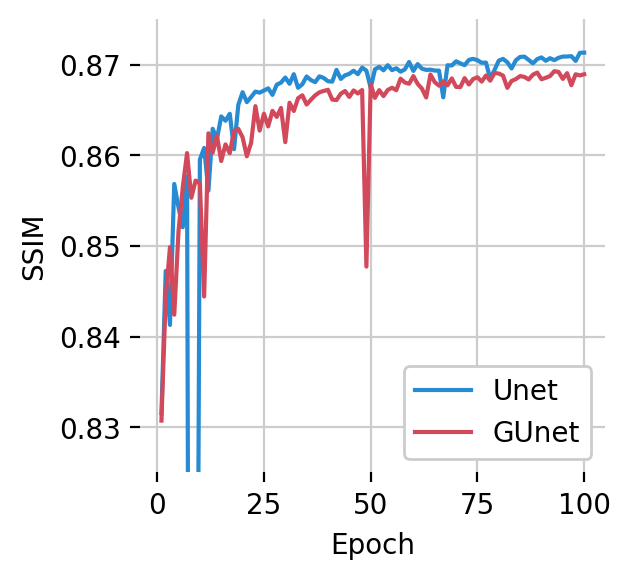
\includegraphics[width=\textwidth]{images/val_ssim_epoch.png}
        \caption{\label{fig:val_ssim_epoch}}
    \end{subcaptionblock}
    \begin{subcaptionblock}[t]{0.49\textwidth}
        \centering
        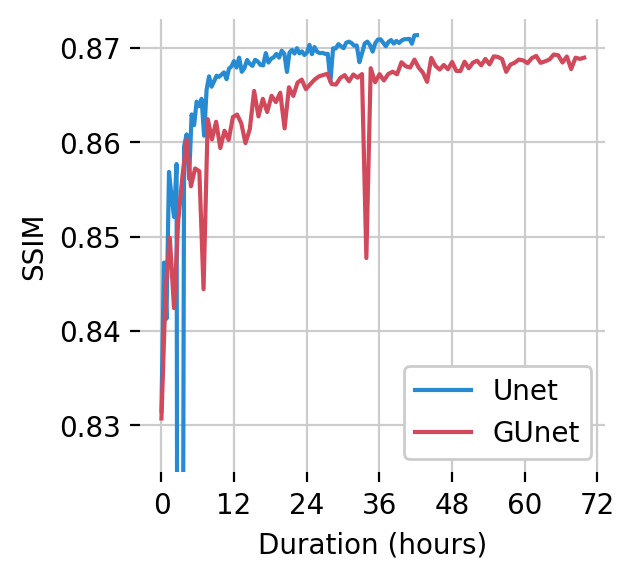
\includegraphics[width=\textwidth]{images/val_ssim_duration.png}
        \caption{\label{fig:val_ssim_duration}}
    \end{subcaptionblock}
    \begin{subcaptionblock}[t]{0.49\textwidth}
        \centering
        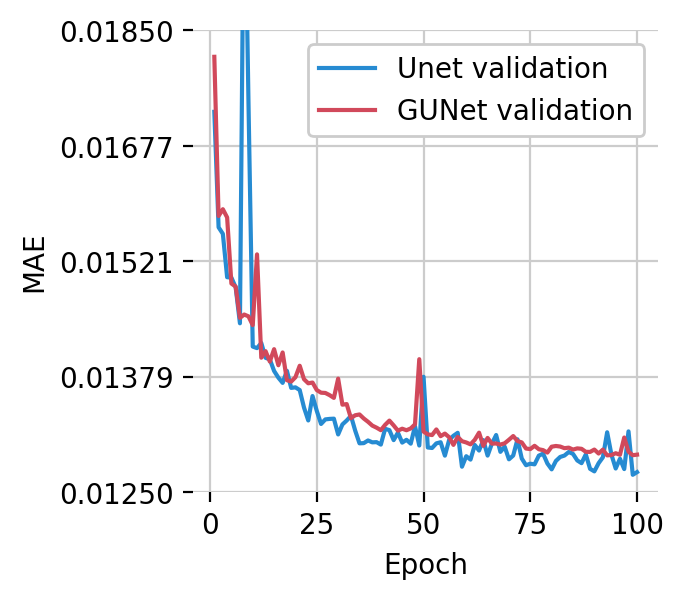
\includegraphics[width=\textwidth]{images/val_mae_epoch.png}
        \caption{\label{fig:val_mae_epoch}}
    \end{subcaptionblock}
    \begin{subcaptionblock}[t]{0.49\textwidth}
        \centering
        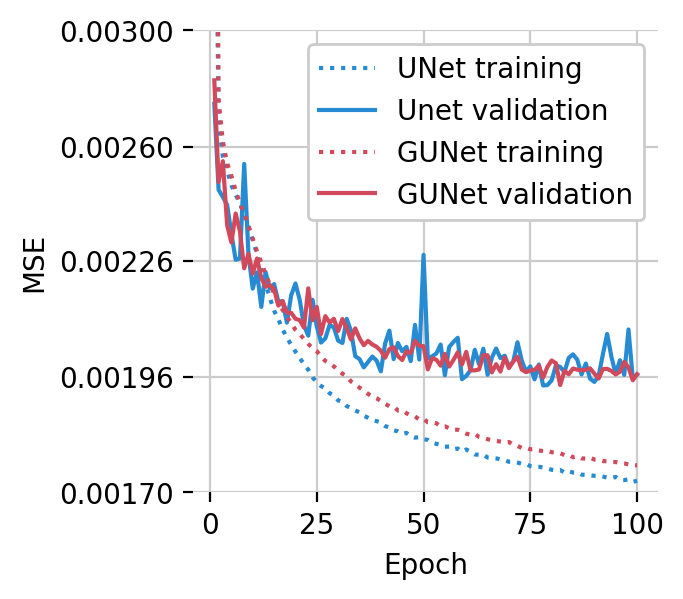
\includegraphics[width=\textwidth]{images/train_val_mse_epoch.png}
        \caption{\label{fig:train_val_mse_epoch}}
    \end{subcaptionblock}
    \captionsetup{subrefformat=parens}
    \caption[Training progress]{\label{fig:training}Training progress quantified by \gls{SSIM}, \gls{MAE} and \gls{MSE}. Relationship between \gls{SSIM} and the number of epochs can be seen in \subref{fig:val_ssim_epoch}, while \subref{fig:val_ssim_duration} shows \gls{SSIM} as a function of training time. \gls{MAE} on the validation dataset is in \subref{fig:val_mae_epoch}. \gls{MSE} was measured on the training data, too, as it was used as a loss function for training. Comparison between training and validation loss can be seen in \subref{fig:train_val_mse_epoch}.}
\end{figure}
\chapter{Evaluation and Results}
\label{chap:evaluation_results}

Models that achieved the best validation \gls{SSIM} values during the training were analyzed. For the investigation, I used the third distinct dataset. I used full resolution 544×352 images, without cropping, as the factors of the image sides are $544 = 2^5\times 17^1$ and $352 = 2^5\times 11^1$. Therefore the five max-pooling layers with 2×2 kernel and 2×2 will behave the same as in training. I tested the models in evaluation mode and on the same metrics as in the section \ref{subsec:training}. While the models in evaluation mode are not inherently stochastic, they can introduce some level of randomness if there are any numerical instabilities during the computation. I ran ten tests on the dataset to obtain accurate results and calculated the average. Average values over the runs for the UNet were:

\begin{align*}
    &\texttt{\gls{SSIM}}: 0.8784421, & &\texttt{\gls{MAE}}: 0.0126786, & &\texttt{\gls{MSE}}: 0.0021389
\end{align*}

\noindent and for the \gls{GUNet} were:
\begin{align*}
    &\texttt{\gls{SSIM}}: 0.8782260, & &\texttt{\gls{MAE}}: 0.0125654, & &\texttt{\gls{MSE}}:0.0020741.
\end{align*}

\section{Comparison of Forecasts}
\label{sec:comparison}

Both networks generally fail to predict the location of the most intense storms and tend to spread the higher-intensity clusters more and more as the predictions advance. To present the differences in the weather forecasts produced by the models, I created a visualization of the outputs side by side with the observed weather phenomena. I decided to crop all the ground truth observations and network outputs to images with resolution 256×256, as portrayed in figure \ref{fig:comparison_06_cutout}, to better visualize the cloud structure.

\begin{figure}[ht]
    \centering
    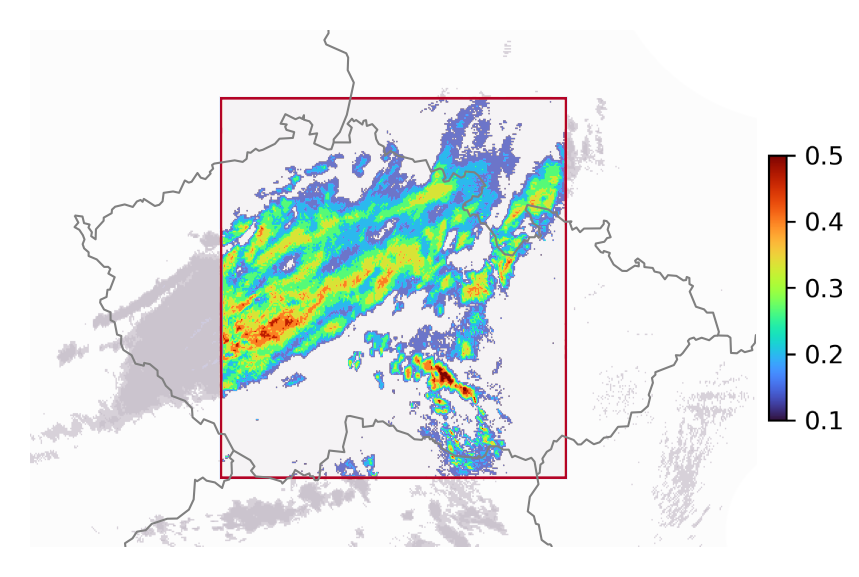
\includegraphics[width=\textwidth]{images/comparison_square_06_cutout.png}
    \caption[Cutout which was used for the comparisons of predictions]{\label{fig:comparison_06_cutout}Cutout which was used for images in figure \ref{fig:comparison_06}.}
\end{figure}

 For further improvements in the visual comparison, I restricted the color bar in the visualization to only show values between lower bound $l$ and upper bound $h$. I adjusted the alpha value of each pixel $x$ in each image to have the value:

\begin{equation}
    \text{f}(x)=\max\left(0,\tanh\left(4\pi\frac{\left(x-l\right)}{h-l}\right)\right).
\end{equation}

 The alpha values guarantee a smooth change to transparency when the pixel's value approaches $l$. If a pixel's value is greater than $h$, it is adjusted to match the value of $h$.

Figure \ref{fig:comparison_06} illustrates the predictions made by \gls{GUNet} and UNet for a particular set of inputs and targets. Only four out of the eight targets and outputs are displayed, while the inputs are not shown. The predictions are spaced 20 minutes apart, enabling more evident observation of cloud movement and future prediction changes. The \gls{SSIM} and \gls{MAE} computed from the cutouts are provided below each prediction.

To see additional examples, please refer to figures \ref{fig:comparison_01}, \ref{fig:comparison_09}, \ref{fig:comparison_07}, and \ref{fig:comparison_04} in appendix \ref{apx:comparisons}. In figure \ref{fig:comparison_01}, you will find a situation with higher-intensity radar echoes, while figure \ref{fig:comparison_09} displays more complex cloud formations on radar images. The other images were chosen from a randomized batch of data points from the test dataset to ensure an unbiased selection. To guarantee that the images included radar echoes, To sort the data points, I utilized the mean value of the pixels in the inputs and then chose the images that had the highest mean values.

\begin{figure}[H]
    \centering
    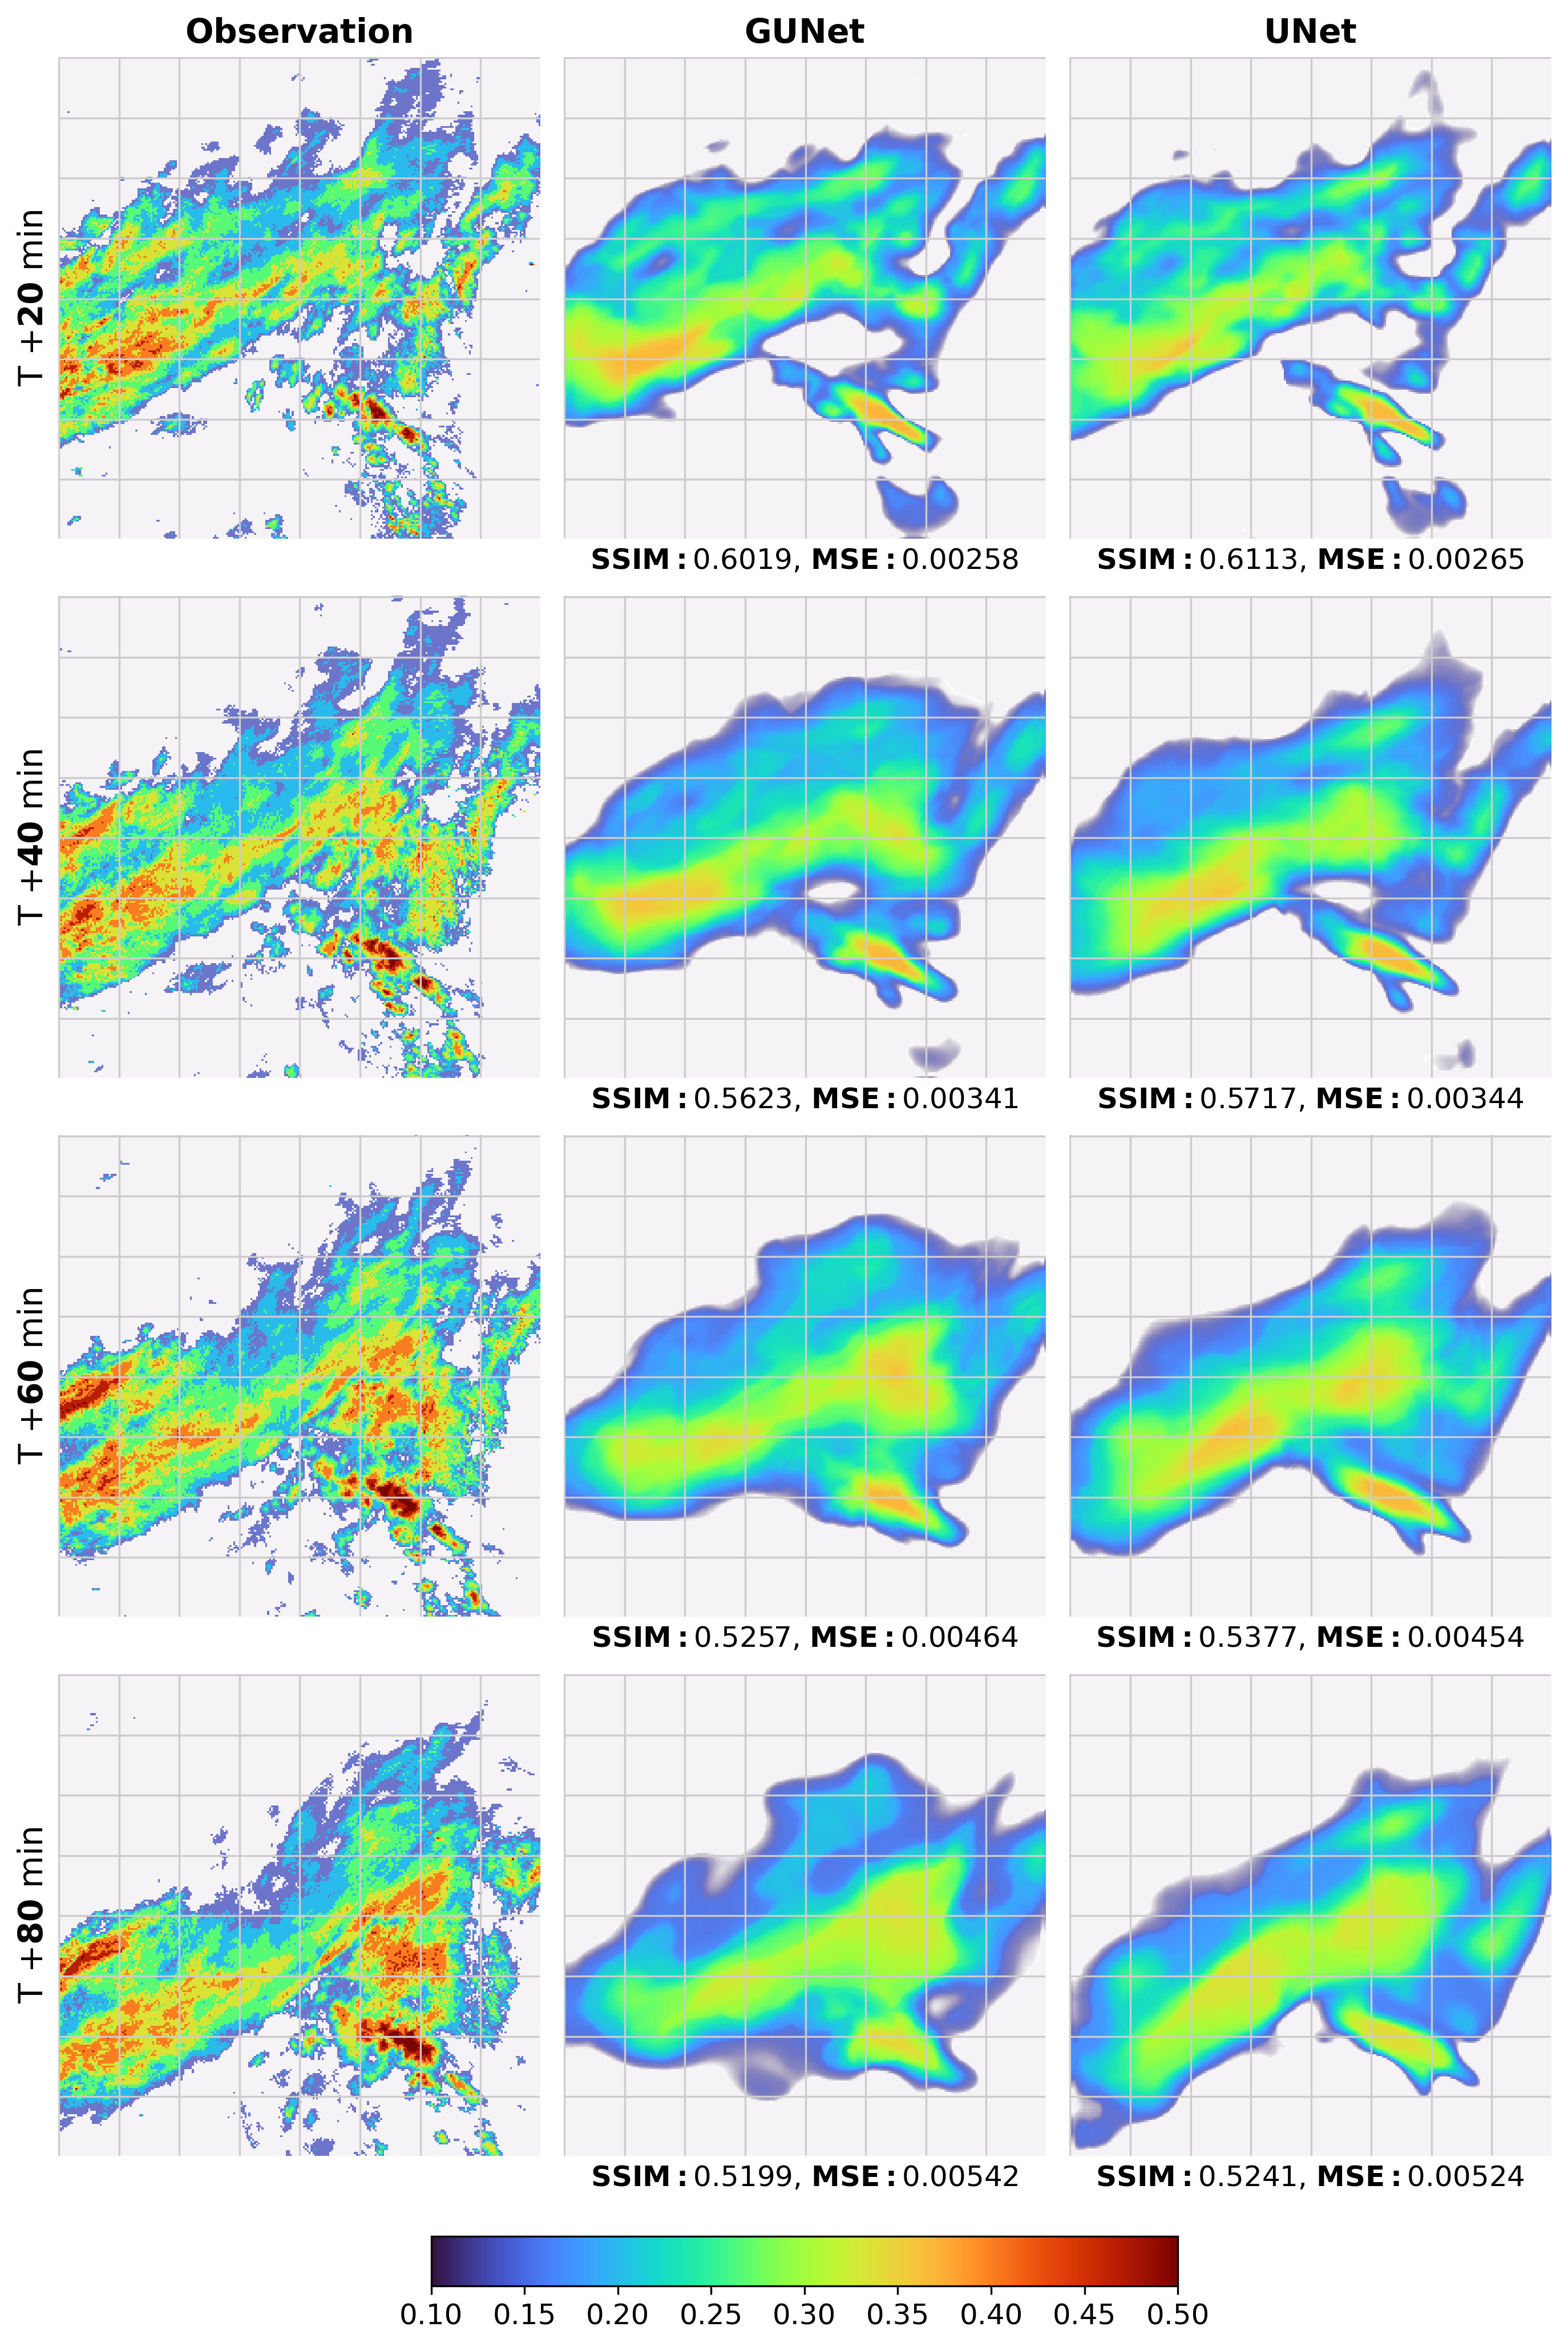
\includegraphics[width=\textwidth]{images/comparison_square_06.png}
    \caption[Comparison of weather predictions of both models (1)]{\label{fig:comparison_06}Comparison of UNet and GUnet outputs with ground truth observations.}
\end{figure}

\subsection{Forecast of Higher Intensity Storms}
\label{sec:forecast_higher_intensity}

To evaluate the performance of the models on higher-intensity storms, I set the values in the output and target tensors to 0 if they were below some threshold. I measured the metrics \gls{SSIM}, \gls{MAE}, and \gls{MSE} for different threshold values on the test dataset, the same way as I mentioned at the beginning of the chapter. Figure \ref{fig:threshold_ssim} shows that \gls{GUNet} achieved better performance than the UNet when $\texttt{threshold} \geq 0.2$.

As the threshold increases, fewer pixels are available for model comparison, leading to a decrease in performance differences between the models. At a $\texttt{threshold} \approx 0.35$, both models achieved the same level of performance in all metrics. Therefore, the discrepancy observed at $\texttt{threshold} = 0.2$ is unrelated to the natural decrease of the differences. If the threshold is high enough, both models can achieve an MSE and MAE of 0 and an SSIM of 1. The appendix includes figures \ref{fig:threshold_mae} and \ref{fig:threshold_mse}, demonstrating the relationship between threshold and \gls{MAE} and \gls{MSE}.


\begin{figure}[ht]
    \centering
    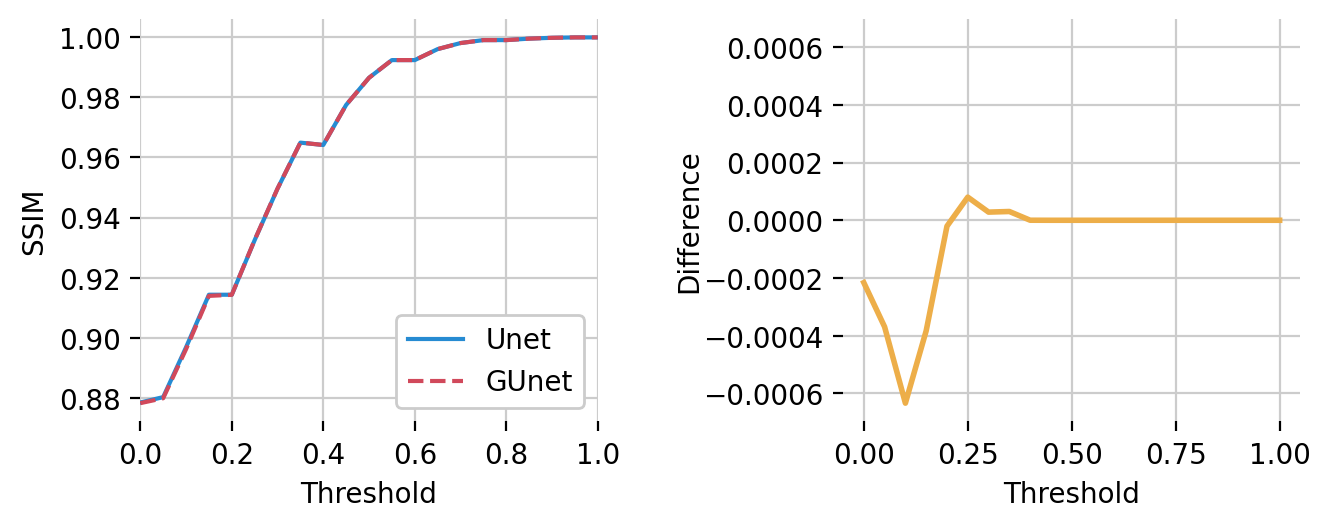
\includegraphics[width=\textwidth]{images/threshold_ssim.png}
    \caption[Higher intensity storm prediction metrics]{\label{fig:threshold_ssim}The test dataset was used to calculate the average \gls{SSIM}, comparing outputs and targets. Any values below a specified threshold were considered to be 0. The chart on the right displays the difference between $\texttt{ssim\_gunet} - \texttt{ssim\_unet}$ based on the threshold value.  Negative values indicate that UNet performed better in \gls{SSIM}, and positive values indicate that \gls{GUNet} had better \gls{SSIM}.}
\end{figure}

\section{Impact of Guided Upsampling on Spectral Bias}
\label{sec:impact_guided_upsampling}

In order to determine whether the \gls{GU} had any influence on the spectral bias by eliminating the structural bias\footnote{Reasoning behind this hypothesis was explained in section \ref{sec:bias}}, I followed a similar method to the one in the paper \cite{gunet}. I compared the average Fourier spectra of the targets and both models. I did this by averaging all outputs over the whole test dataset and computing a spectrum of the average using a 2D Fourier transform, equivalent to computing the Fourier spectra for each image and averaging that\footnote{The reason behind it is the linearity of the Fourier transform}. Let $\mathcal{D} = \{d_1, d_2, \dots, d_N\}$ be the set of data points, where each $d_i = \{I_{i1}, I_{i2}, \dots, I_{i8}\}$ represents a set of 8 images. I defined the function $\texttt{AvgMagSpectrum}$ to compute the magnitude spectrum of the average images across all data points and within each data point:

\begin{equation}
    \texttt{AvgMagSpectrum}(\mathcal{D}) = \left| \mathcal{F} \left( \frac{1}{8N} \sum_{i=1}^{N} \sum_{j=1}^{8} I_{ij} \right) \right|,
\end{equation}

\noindent where $\mathcal{F}\{\cdot\}$ denotes the Fourier Transform, and $|\cdot|$ represents the magnitude of the complex Fourier coefficients.

The function can be applied to the sets $\mathcal{D}_{\texttt{GUNet}}$, $\mathcal{D}_{\texttt{UNet}}$, and $\mathcal{D}_{\texttt{tgt}}$ to compute the magnitude spectra $\bar{M}_{\texttt{GUNet}}$, $\bar{M}_{\texttt{UNet}}$, and $\bar{M}_{\texttt{tgt}}$ for the respective \gls{GUNet} outputs, UNet outputs, and targets. After computing the magnitude spectra, the zero-frequency component was shifted to the center of the spectrum for better visualization and analysis. $\bar{M}_{\texttt{GUNet}}$, $\bar{M}_{\texttt{UNet}}$, and $\bar{M}_{\texttt{tgt}}$ are displayed in figure \ref{fig:fourier}.

\begin{figure}[ht]
    \centering
    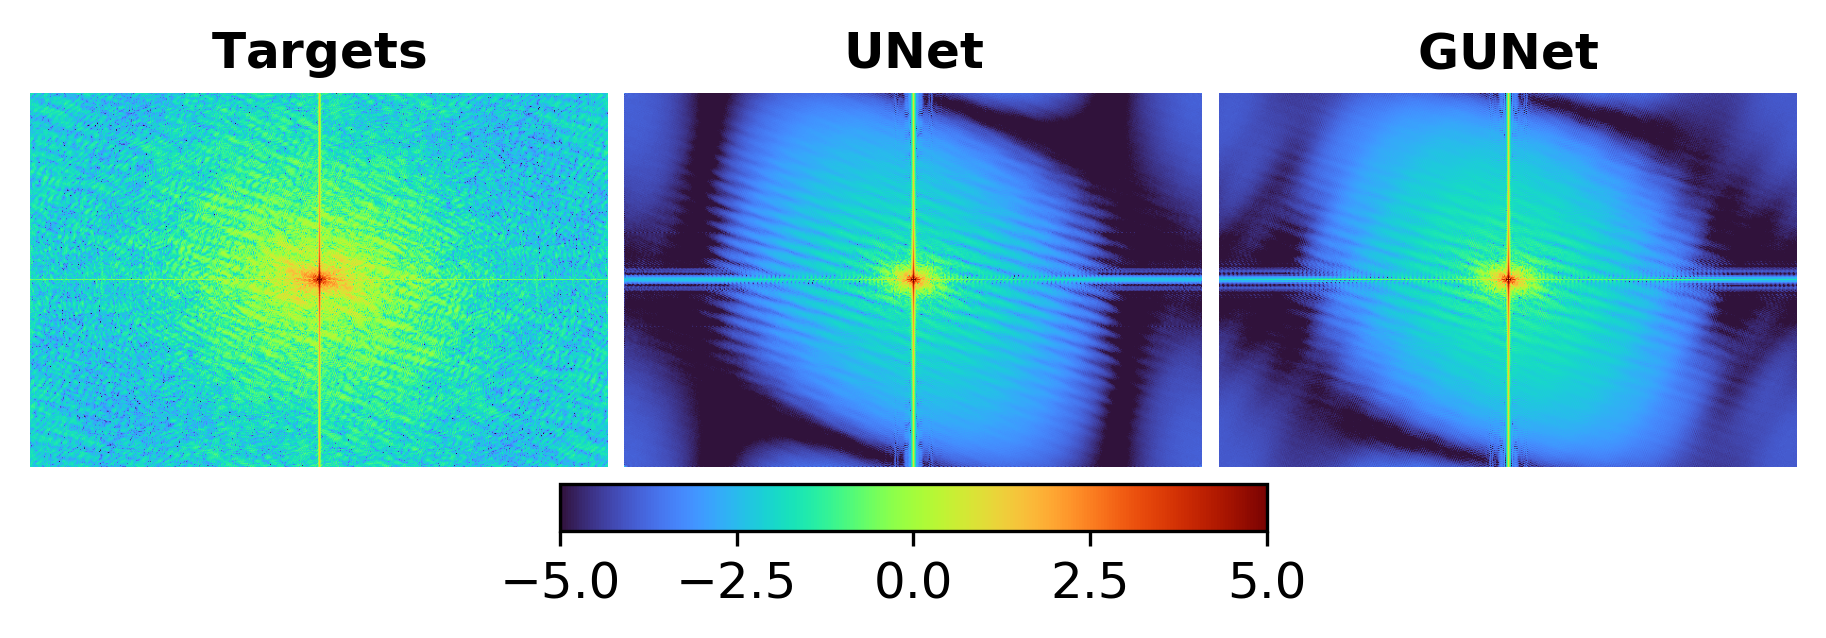
\includegraphics[width=\textwidth]{images/fourier.png}
    \caption[Comparison of average fourier spectra]{\label{fig:fourier}Average magnitude spectrum of UNet outputs $\bar{M}_{\texttt{UNet}}$, GUnet outputs $\bar{M}_{\texttt{GUNet}}$ and ground truth $\bar{M}_{\texttt{tgt}}$ on a logarithmic scale.}
\end{figure}

At first glance, the differences may not be immediately apparent. \gls{GUNet} seems to capture more of the higher frequencies\footnote{Higher frequencies are the ones further away from the center.}. To investigate this more thoroughly, I calculated the absolute value of the difference between the average spectrum of the targets and the average spectrum of the network outputs by computing:

\begin{equation}
    \texttt{diff}\left(\bar{M}_{m}\right)=\left| \bar{M}_{\texttt{tgt}} - \bar{M}_{m} \right|,
\end{equation}

\noindent where $\bar{M}_{m}$ is $\bar{M}_{\texttt{UNet}}$ or $\bar{M}_{\texttt{GUNet}}$. The result of this can be seen in figure \ref{fig:fourier_diff_1}. In the appendix  \ref{apx:comparisons}, I included figure \ref{fig:fourier_diff_2}, which shows a different plot of the same data, and figure \ref{fig:fourier_diff_3} that shows the difference between the output spectra of both models. Values were passed through moving average with a window size of 32×32, so the differences between the two spectra can be seen more clearly.

\begin{figure}[ht]
    \centering
    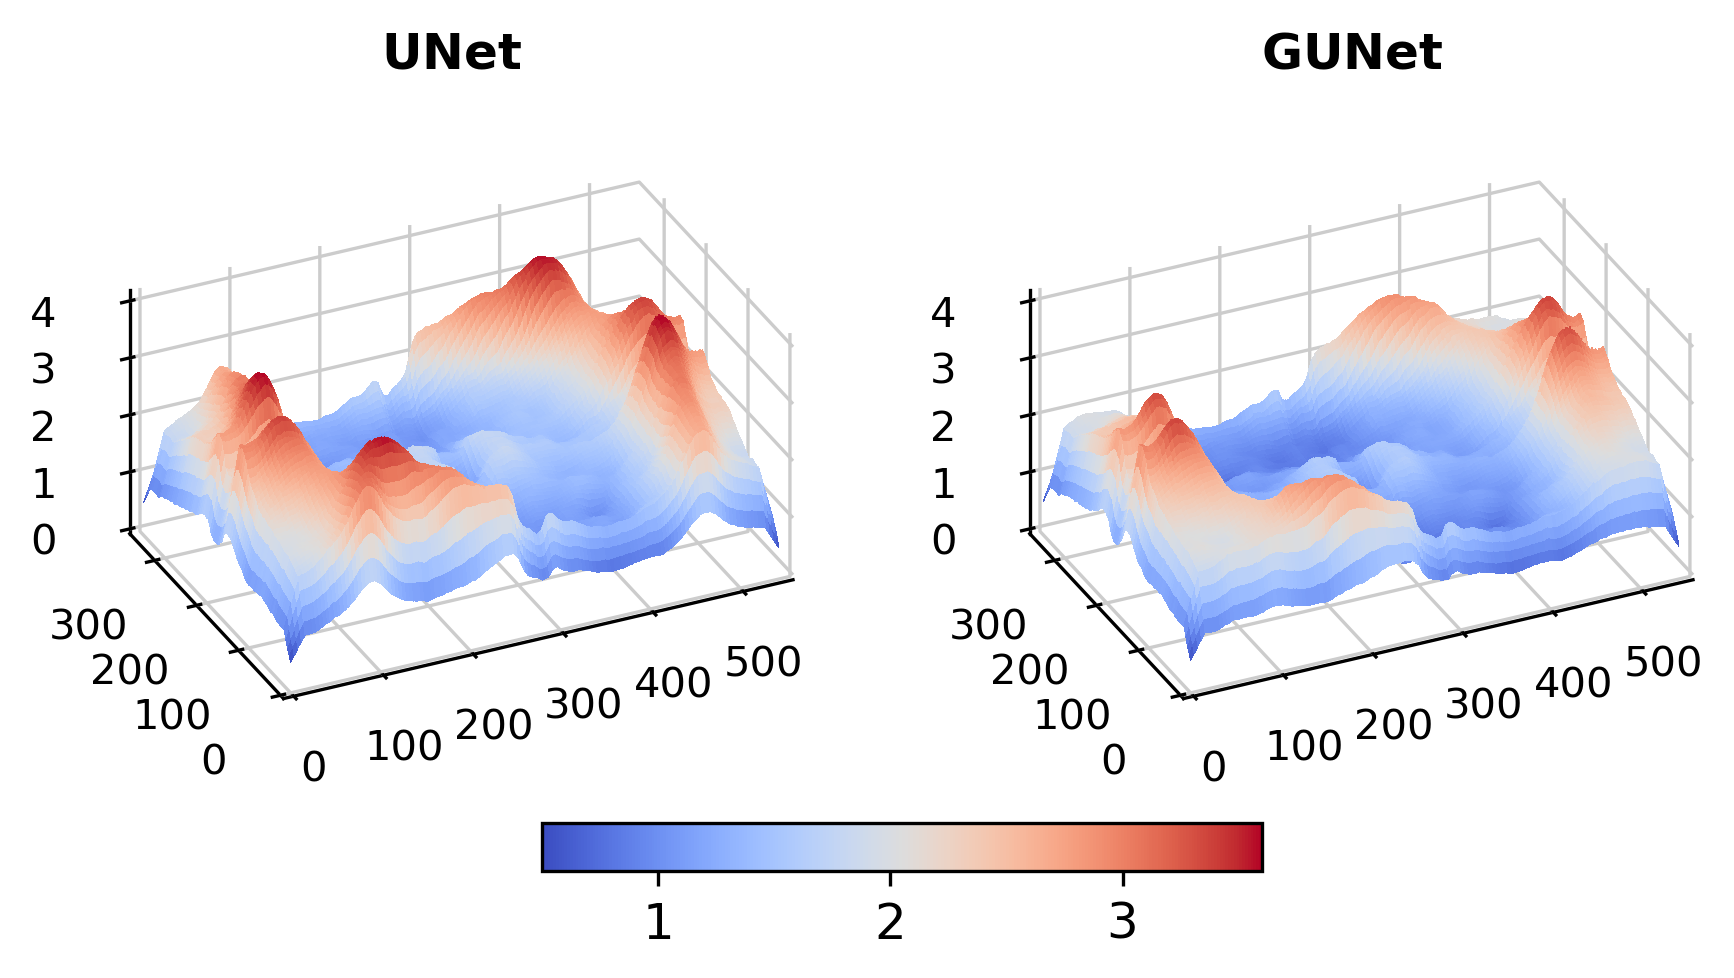
\includegraphics[width=\textwidth]{images/fourier_diff_1.png}
    \caption[Difference between the target and output spectra (3D plot)]{\label{fig:fourier_diff_1}Absolute difference between the amplitudes of the average target spectrum and the average output spectra of models on a logarithmic scale. Values were smoothed by moving average with kernel size 32×32. An unsmoothed 2D chart is in figure \ref{fig:fourier_diff_2}. A higher pixel value means that the amplitude, at the frequency corresponding to that pixel, differed more from the desired amplitude of the average target spectrum.}
\end{figure}


\chapter{Discussion}
\label{chap:discussion}


\section{Interpretation of Results}
\label{sec:interpretation}

From the average Fourier spectrum of the UNet $\bar{M}_{\texttt{UNet}}$ in figure \ref{fig:fourier} is clear that the network did not produce the structural artifacts\footnote{See the section \ref{subsec:structural_bias}.} because it produced $\bar{M}_{\texttt{UNet}}$ without the checkerboard-like structure which was present in results of a similar experiment in the paper \cite[fig. 3]{gunet}. The UNet in the paper\footnote{The paper \cite{gunet} presents various UNet architectures. Specifically, I am talking about the one called Transposed Convolution UNet or``TC-UNet," as named in the paper.} utilized a 4x4 kernel in their transposed convolution, while my UNet used a 2x2 kernel\footnote{Size of the kernel was found in hyperparameter search. See section \ref{subsec:hyperparameters}.}.

The smaller kernel may have helped to mitigate the artifacts since with 2×2 kernel with a 2×2 stride means that each pixel in the output of the transposed convolution is a function of just one input pixel. Whereas with a 4×4 kernel and the same stride, each output pixel is affected by four input pixels. In contrast, the \gls{GIF} in \gls{GUNet} was used with $\texttt{radius} = 2$, which means that output pixels are assumed to be a linear transformation of the input image with coefficients computed on a window $\omega_k$, so in the case of $\texttt{radius} = 2$, the size of this window is $\left|\omega_k\right| = \left(2r + 1\right)^2 = 25$.

UNet may have learned to mitigate these artifacts, or they were not created due to the tiny kernel. Either way, it may have been at the expense of worse performance than the \gls{GUNet} when I compare the average \gls{MAE} and \gls{MSE} on the test dataset. While the UNet was better in both metrics on the validation dataset, on the test dataset, \gls{GUNet} outperformed the UNet. The \gls{SSIM} is also interesting to compare. UNet scored better, but the margin has shrunk ten times from 0.002 to 0.0002. Intriguingly, the \gls{SSIM} values improved on the testing dataset. The reason behind it could be the randomness in creating the datasets. Both networks were tested and trained on the same datasets so they could be compared on them. The \gls{SSIM} on the validation dataset has practically only risen during training, so it is unlikely that overfitting of the UNet is the reason for its declined performance. However, it has more parameters than the GUNet, which would make it more likely to do so.

Another critical difference between the models, which can be seen in the results, is the ability of the \gls{GUNet} to capture higher frequencies than the UNet. By itself, capturing higher frequencies does not imply better weather predictions, but the improvement is significant because of the spectral bias present in \glspl{NN}\footnote{I. e. tendency of neural networks to learn lower frequencies more easily. See the section \ref{subsec:spectral_bias}.} .

Weather nowcasting aims to anticipate severe weather conditions and safeguard us from dangers caused by rapidly changing weather patterns. In this regard, predicting high-intensity levels in radar images is more advantageous. Figures \ref{fig:threshold_ssim}, \ref{fig:threshold_mae}, and \ref{fig:threshold_mse} indicate that the performance of the \gls{GUNet} was superior to that of the UNet in images where lower intensities were removed. Although the improvement was relatively small, as shown in the figures.

Granting all these differences, when the weather predictions of both networks are compared to the target predictions, they look nearly identical.

\section{Limitations and Potential Improvements}
\label{sec:limitations_improvements}

My approach has some limitations, some of which I already mentioned earlier. Firstly, I did not remove nearly empty images from the dataset, which may have impacted the training time and the performance of the models.

The second limitation I already mentioned is padding in the convolutions. If I instead allowed the convolution outputs to decrease each time, the network's final output would be much smaller than the input, but it would lead to better performance around the edges of the image.

Next, I would improve the speed of the GUNet. In the implementation of \gls{GUNet}, I used the standard \gls{GIF} algorithm \ref{ax:gif}, but there is a faster algorithm \ref{ax:gif_fast}, which may improve the long training time observed in the figure \ref{fig:val_ssim_duration}.

Finally, while the differences in the performance of the models are there, it is paramount to mention that they were observed on just one pair of networks and trained only once, which means that the results are not statistically significant and to obtain more definite outcomes, additional, comprehensive research is necessary. This research could involve exploring additional hyperparameters, like varying kernel sizes in each layer and parameterizing the model depth. The search for hyperparameters could also be longer, letting the networks run for more epochs. Final training could be done for more epochs and multiple times. Different, more complex loss functions could also be tried.




\setsecnumdepth{part}
\chapter{Conclusion and Future Work}
\label{chap:conclusion}

This thesis has sought to enhance the accuracy and reliability of short-term weather predictions, notably storm structure predictions from radar images, by addressing the structural biases present in deep learning models like the UNet architecture. By adapting and applying the Guided Upsampling technique from the Guided UNet (GUNet) architecture to weather nowcasting, I could effectively mitigate the adverse effects of transposed convolution on weather predictions. This approach led to the development of a more spectrally consistent model.

Through a comprehensive literature review, the reader was introduced to the concepts of weather nowcasting, \glspl{CNN}, the UNet architecture, \gls{GIF}, and spectral bias. A dataset of radar composites from a network of weather radars created by \gls{OPERA} was utilized for training and evaluating the \gls{GUNet} and UNet models. The impact of \gls{GU} was analyzed on the \gls{GUNet} and UNet models using metrics such as \gls{MSE}, \gls{MAE}, and \gls{SSIM}.

The results demonstrated that, while the UNet successfully mitigated the structural artifacts, the \gls{GUNet} model outperformed it in terms of average \gls{MAE} and \gls{MSE} on the test dataset. Additionally, the \gls{GUNet} demonstrated an improved ability to capture higher frequencies compared to the UNet, which is a significant finding considering the spectral bias issue in neural networks.

Despite the improvements observed in the \gls{GUNet} model, some limitations and potential improvements were identified, including the removal of nearly empty images from the dataset, addressing padding in convolutions, improving the speed of the \gls{GUNet} using a faster \gls{GIF} algorithm, and conducting a more exhaustive investigation of the models by multiple training runs with more hyperparameters.

The implications for weather nowcasting suggest that the \gls{GUNet} model's improved performance on images with higher radar echo intensities may contribute to better predictions of severe weather events, which are of utmost importance for public safety and infrastructure protection. Although the performance improvement is relatively small, it still signifies progress in the ongoing efforts to create more precise and dependable weather forecasts.

In conclusion, this thesis has successfully, even if marginally, advanced the field of weather nowcasting by addressing structural biases in convolutional neural networks used in this field.


\section{Summary of Findings}

The key findings of this thesis are as follows:
\label{sec:summary_findings}

\begin{itemize}
    \item The \gls{GUNet} model, which incorporates \gls{GU}, demonstrated improved performance compared to the UNet model in terms of average \gls{MAE} and \gls{MSE} on the test dataset while achieving nearly identical average \gls{SSIM}, which suggests that the \gls{GUNet} model provides a marginal improvement in accurate and reliable short-term weather predictions from radar images.
    \item The \gls{GUNet} model more successfully captured higher spatial frequencies than the UNet model.
    \item The \gls{GUNet} model performed better than the UNet model on images with higher radar echo intensities, which is particularly important for predicting severe weather events in the context of weather nowcasting.
\end{itemize}

\section{Future Research Directions}
\label{sec:future_research}

Based on the findings and limitations of this thesis, the following future research directions are proposed:
\begin{itemize}
    \item More extensive hyperparameter searches, including parameters such as model depth and different kernel sizes in each layer, could lead to a better comparison of both models and improvements in performance.

    \item Utilizing a faster \gls{GIF} algorithm in the GUNet model could reduce training time, allowing for more extensive experimentation and potentially better model performance in the same training time. Removing nearly empty images from the dataset could also lead to similar improvements.

    \item Testing different, more complex loss functions may improve the model's ability to predict storm structures and contribute to more accurate and reliable weather forecasts.

    \item Investigating if using \gls{GIF} in other deep learning models and techniques, such as recurrent \glspl{GAN} or stable diffusion, could improve their performance.

\end{itemize}




\bibliographystyle{iso690}
\bibliography{bibliography}

\setsecnumdepth{all}
\appendix

\chapter{Guided Image Filtering algorithms}
\label{ax:gif}
% \printglossaries
\section{Guided Filter}

\begin{algorithmic}
    \State \textbf{Input:} \phantom{1}\parbox[t]{\dimexpr\linewidth-\algorithmicindent-7em}{
    filtering input image $p$, guidance image $I$, radius $r$,\\
    regularization $\epsilon$
    }
    \vspace{0.1em}

    \State \textbf{Output:} \phantom{1}\parbox[t]{\dimexpr\linewidth-\algorithmicindent-7em}{
    filtering output $q$
    }
    \vspace{0.1em}
    \State \textbf{1:} \phantom{1}\parbox[t]{\dimexpr\linewidth-\algorithmicindent-1em}{
    $\texttt{mean}_I = f_\texttt{mean}(I, r)$ \\
    $\texttt{mean}_p = f_\texttt{mean}(p, r)$ \\
    $\texttt{corr}_{I} = f_\texttt{mean}(I .* I, r)$ \\
    $\texttt{corr}_{Ip} = f_\texttt{mean}(I .* p, r)$
    }
    \vspace{0.1em}
    \State \textbf{2:} \phantom{1}\parbox[t]{\dimexpr\linewidth-\algorithmicindent-1em}{
    $\texttt{var}_I = \texttt{corr}_I - \texttt{mean}_I .* \texttt{mean}_I$ \\
    $\texttt{cov}_{Ip} = \texttt{corr}_Ip - \texttt{mean}_I .* \texttt{mean}_p$
    }
    \vspace{0.1em}
    \State \textbf{3:} \phantom{1}\parbox[t]{\dimexpr\linewidth-\algorithmicindent-1em}{
    $a = \texttt{cov}_{Ip}\ ./\ (\texttt{var}_I + \epsilon)$ \\
    $b = \texttt{mean}_p - a .* \texttt{mean}_I$
    }
    \vspace{0.1em}
    \State \textbf{4:} \phantom{1}\parbox[t]{\dimexpr\linewidth-\algorithmicindent-1em}{
    $\texttt{mean}_a = f_\texttt{mean}(a, r)$ \\
    $\texttt{mean}_b = f_\texttt{mean}(b, r)$
    }
    \vspace{0.1em}
    \State \textbf{5:} \phantom{1}\parbox[t]{\dimexpr\linewidth-\algorithmicindent-1em}{
    $q = \texttt{mean}_a .* I + \texttt{mean}_b$
    }
\end{algorithmic}

\vspace{1em}
The dot before the operation denotes that it is performed elementwise. $f_\texttt{mean}(\cdot, r)$ denotes a mean filter with a radius $r$. Pseudocode was taken from paper \cite{gif}.
\newpage

\section{Fast Guided Filter}
\label{ax:gif_fast}
\begin{algorithmic}
    \State \textbf{Input:} \phantom{1}\parbox[t]{\dimexpr\linewidth-\algorithmicindent-7em}{
    filtering input image $p$, guidance image $I$, radius $r$,\\
    regularization $\epsilon$, subsampling scale $s$
    }
    \vspace{0.1em}
    \State \textbf{Output:} \phantom{1}\parbox[t]{\dimexpr\linewidth-\algorithmicindent-7em}{
    filtering output $q$
    }
    \vspace{0.1em}
    \State \textbf{1:} \phantom{1}\parbox[t]{\dimexpr\linewidth-\algorithmicindent-1em}{
    $I' = f_\texttt{subsample}(I, s)$ \\
    $p' = f_\texttt{subsample}(p, s)$ \\
    $r' = r/s$
    }
    \vspace{0.1em}
    \State \textbf{2:} \phantom{1}\parbox[t]{\dimexpr\linewidth-\algorithmicindent-1em}{
    $\texttt{mean}_{I} = f_\texttt{mean}(I', r')$ \\
    $\texttt{mean}_{p} = f_\texttt{mean}(p', r')$ \\
    $\texttt{corr}_{I} = f_\texttt{mean}(I' .* I', r')$ \\
    $\texttt{corr}_{Ip} = f_\texttt{mean}(I' .* p', r')$
    }
    \vspace{0.1em}
    \State \textbf{3:} \phantom{1}\parbox[t]{\dimexpr\linewidth-\algorithmicindent-1em}{
    $\texttt{var}_{I} = \texttt{corr}_{I} - \texttt{mean}_{I} .* \texttt{mean}_{I}$ \\
    $\texttt{cov}_{Ip} = \texttt{corr}_{Ip} - \texttt{mean}_{I} .* \texttt{mean}_{p}$
    }
    \vspace{0.1em}
    \State \textbf{4:} \phantom{1}\parbox[t]{\dimexpr\linewidth-\algorithmicindent-1em}{
    $a = \texttt{cov}_{Ip}\ ./\ (\texttt{var}_{I} + \epsilon)$ \\
    $b = \texttt{mean}_{p} - a .* \texttt{mean}_{I}$
    }
    \vspace{0.1em}
    \State \textbf{5:} \phantom{1}\parbox[t]{\dimexpr\linewidth-\algorithmicindent-1em}{
    $\texttt{mean}_a = f_\texttt{mean}(a, r')$ \\
    $\texttt{mean}_b = f_\texttt{mean}(b, r')$
    }
    \vspace{0.1em}
    \State \textbf{6:} \phantom{1}\parbox[t]{\dimexpr\linewidth-\algorithmicindent-1em}{
    $\texttt{mean}_a = f_\texttt{upsample}(\texttt{mean}_a, s)$ \\
    $\texttt{mean}_b = f_\texttt{upsample}(\texttt{mean}_b, s)$
    }
    \vspace{0.1em}
    \State \textbf{7:} \phantom{1}\parbox[t]{\dimexpr\linewidth-\algorithmicindent-1em}{
    $q = \texttt{mean}_a .* I + \texttt{mean}_b$
    }
\end{algorithmic}

\vspace{1em}
The dot before the operation denotes that it is performed elementwise. $f_\texttt{mean}(\cdot, r)$ denotes a mean filter with a radius $r$. Pseudocode was taken from paper \cite{fastguided}. Subsampling (nearest-neighbor or bilinear) of the input $p$ and the guidance $I$ by a ratio $s$ is preformed to speed up the guided filter. All the box filters are performed on the low-resolution maps, which are the major computation of the guided filter. The two coefficient maps $\bar a$ and $\bar b$ are bilinearly upsampled to the original size. Finally, the output $q$ is still computed by $q = \bar aI + \bar b$. In this last step, the image $I$ is the full-resolution guidance that is not downsampled, and it will still faithfully guide the output. \cite{fastguided}

\chapter{Model comparisons}
\label{apx:comparisons}


% \begin{figure}[ht]
%     \centering
%     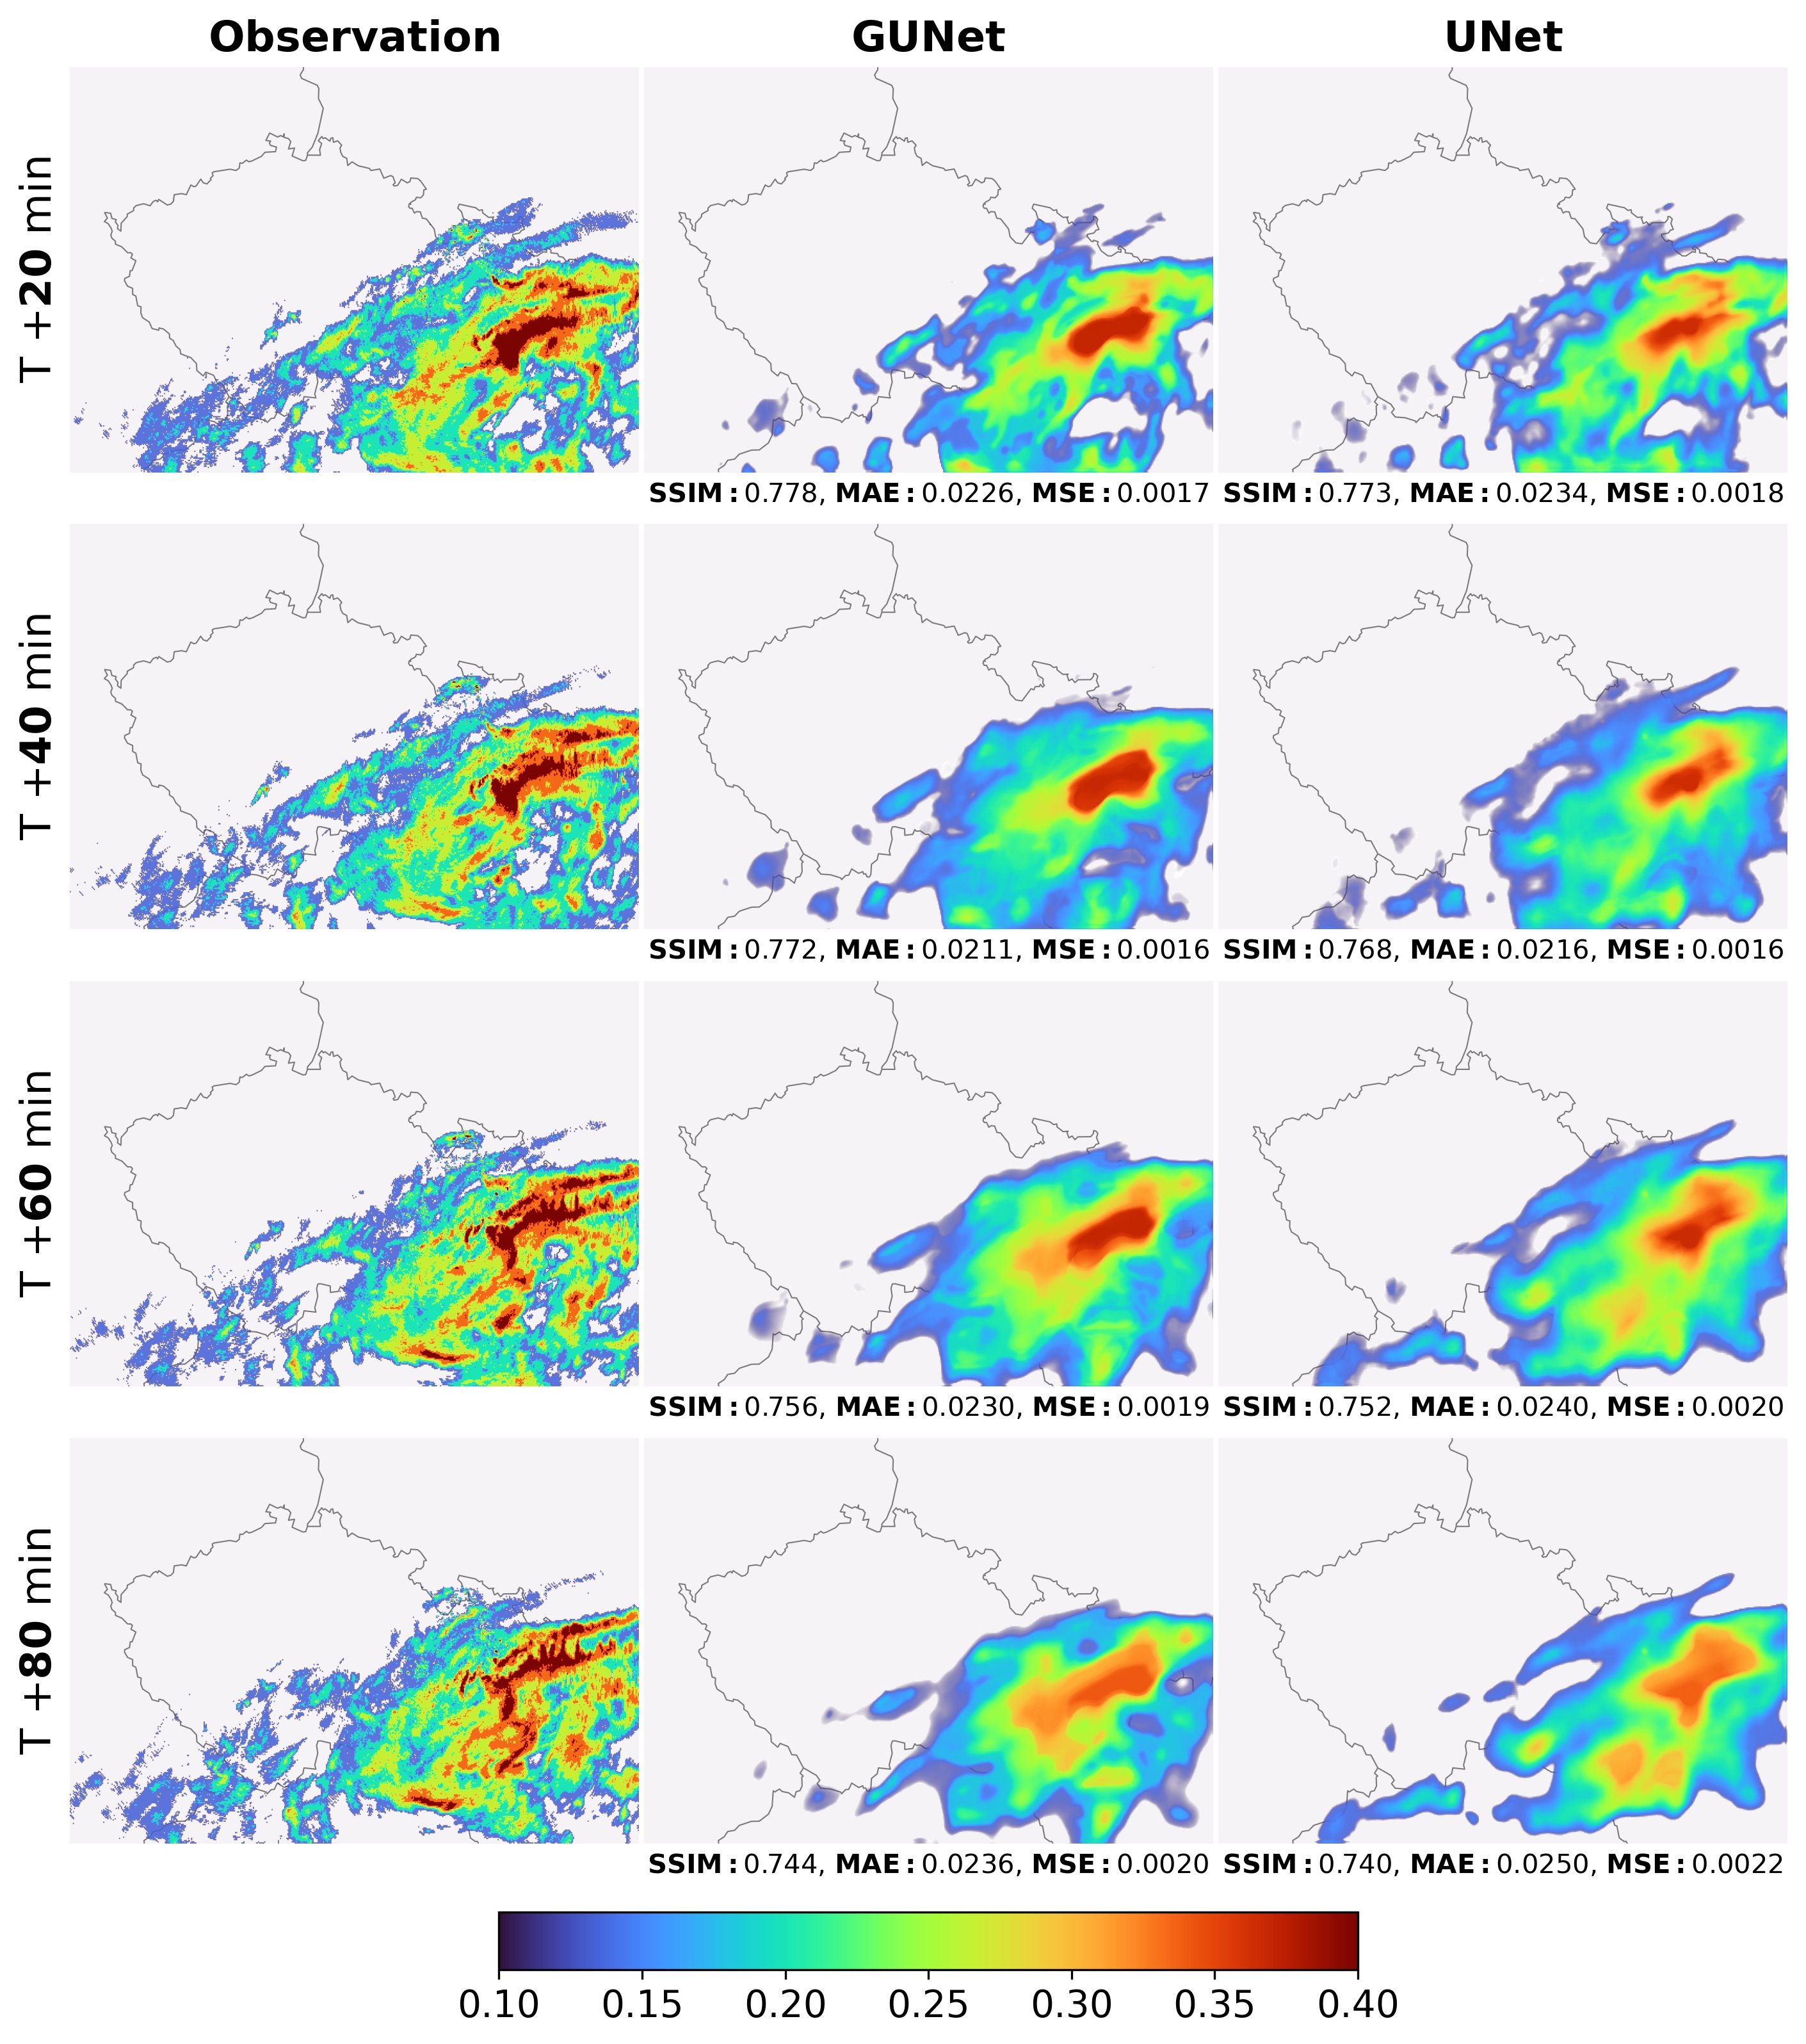
\includegraphics[width=\textwidth]{images/comparison_02.jpeg}
%     \caption[Model comparison on radar images with denser cloud formations]{\label{fig:comparison_02}Model comparison on radar images with denser cloud formations.}
% \end{figure}
%
% \begin{figure}[ht]
%     \centering
%     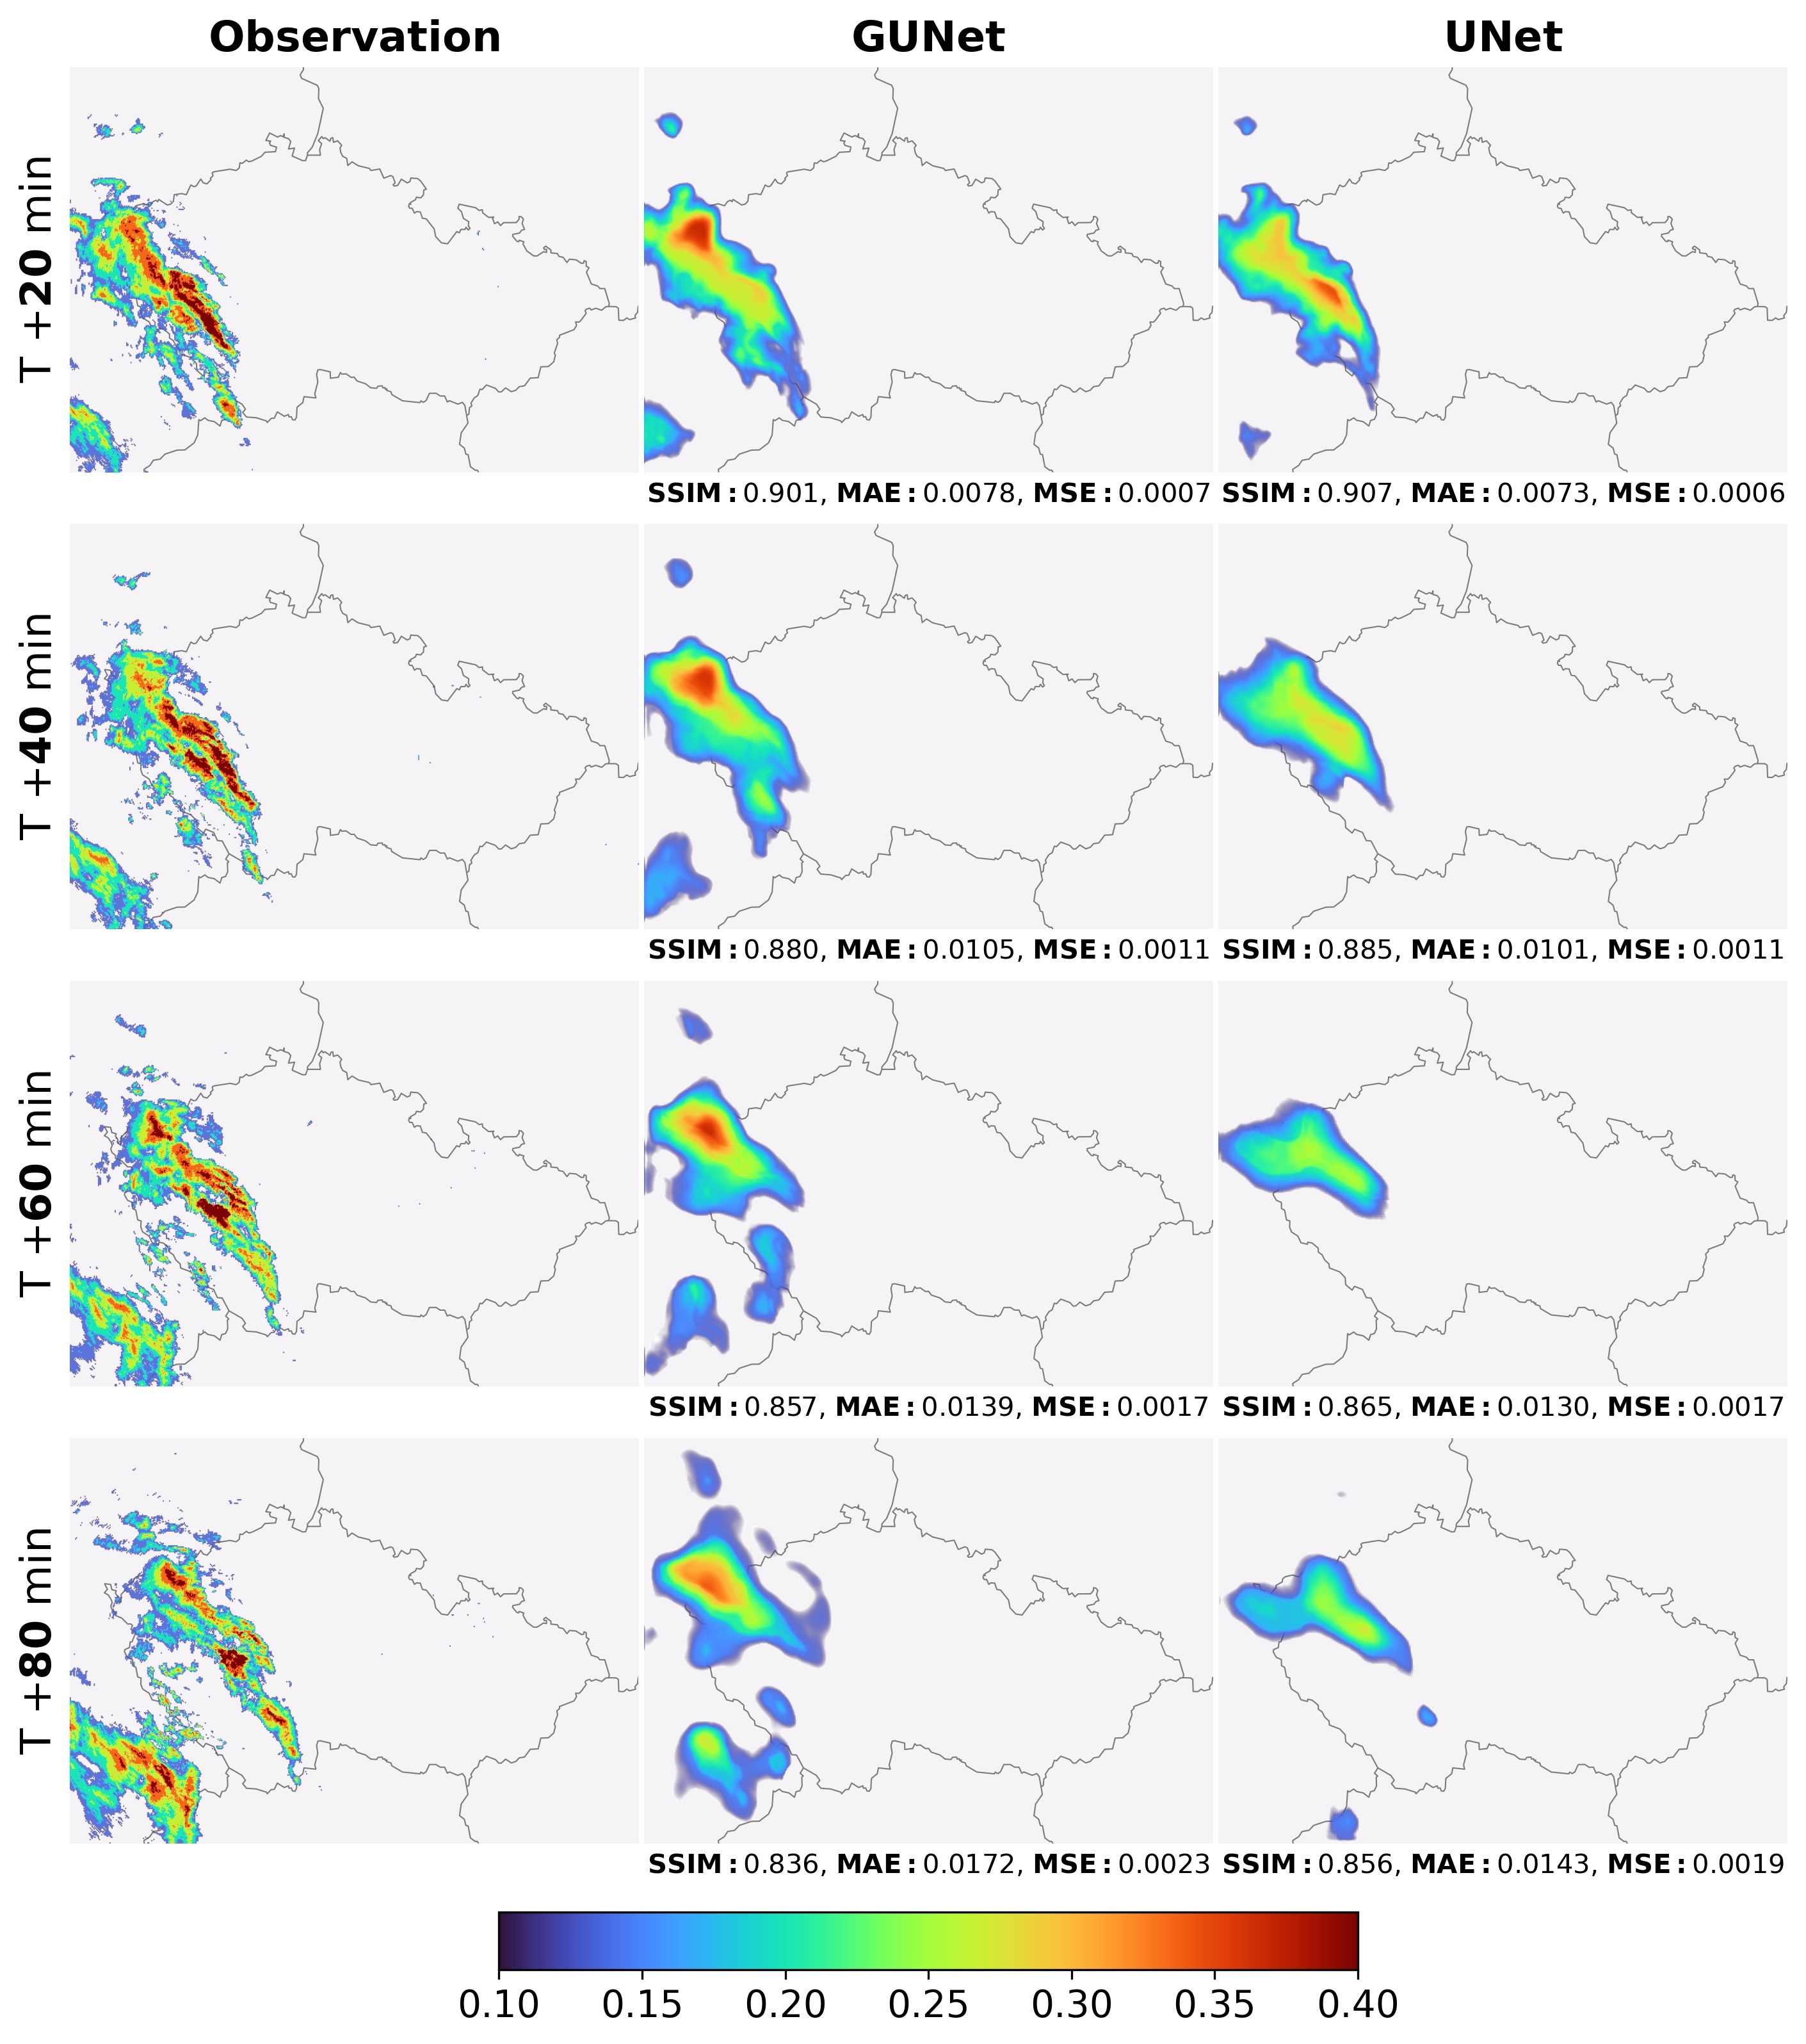
\includegraphics[width=\textwidth]{images/comparison_06.jpeg}
%     \caption[Model comparison on radar images with sparse cloud formations]{\label{fig:comparison_06}Model comparison on radar images with sparse cloud formations.}
% \end{figure}
%
% \begin{figure}[ht]
%     \centering
%     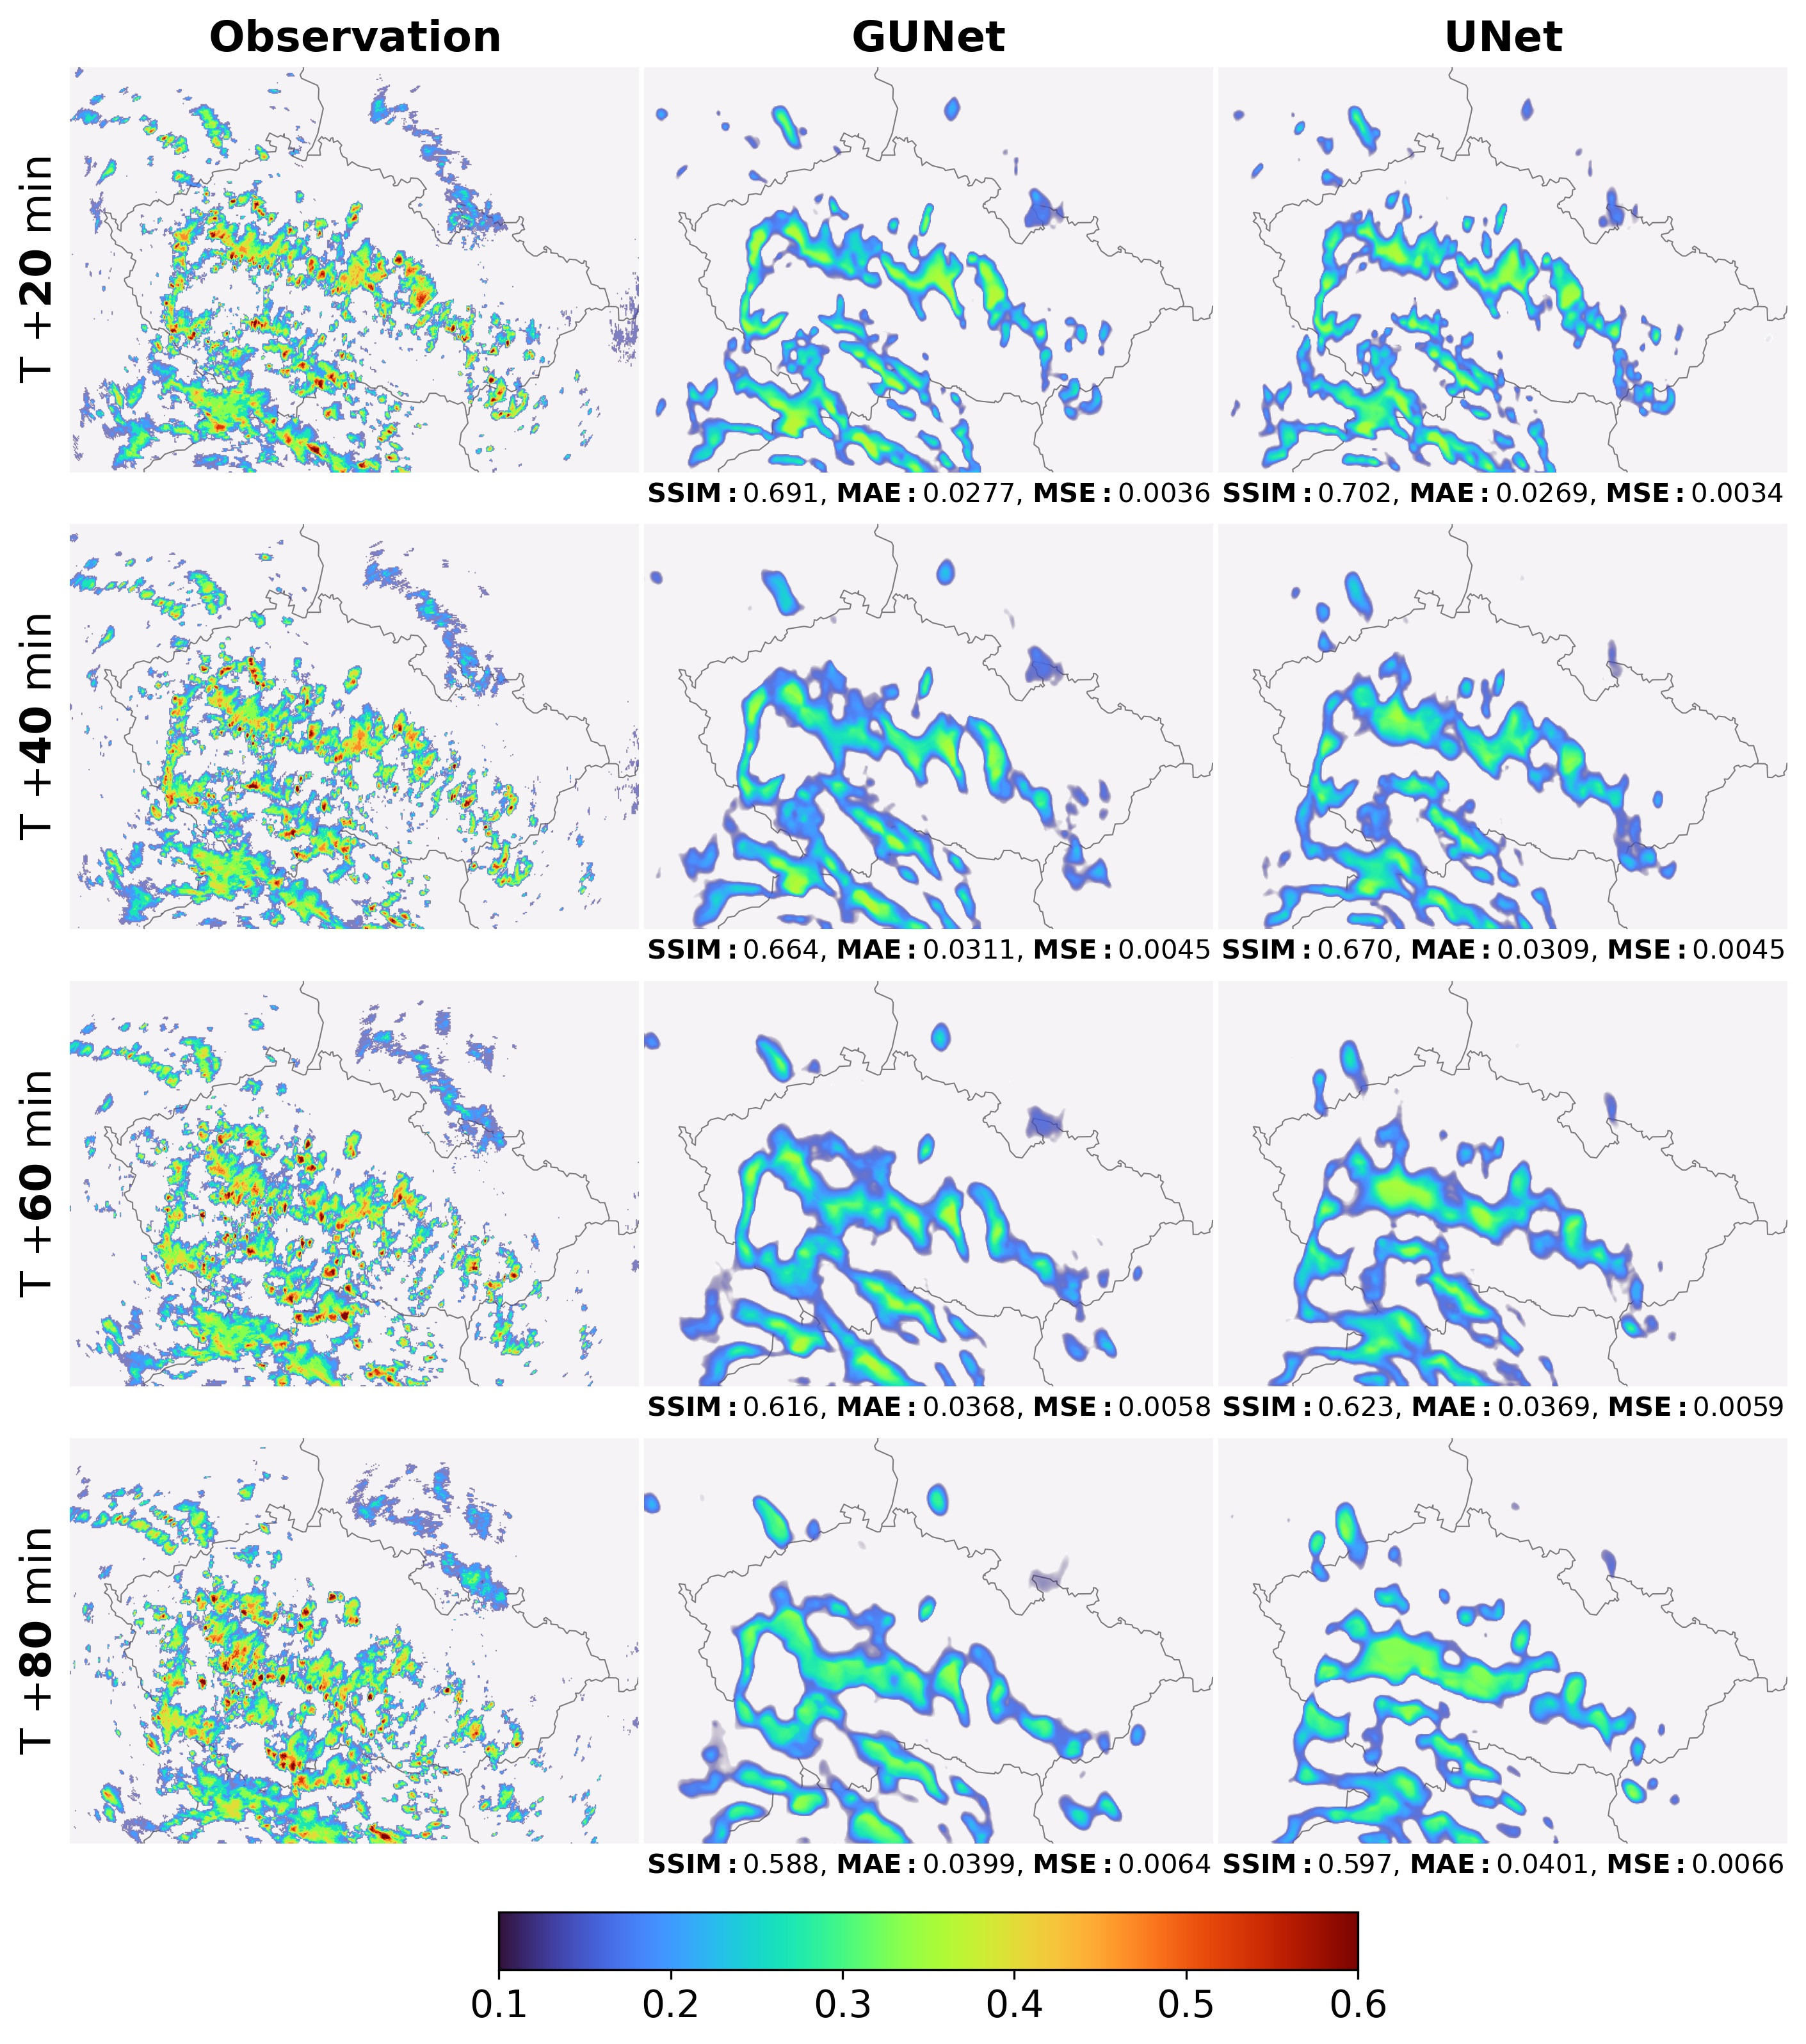
\includegraphics[width=\textwidth]{images/comparison_04.jpeg}
%     \caption[Model comparison on radar images with complex cloud formations]{\label{fig:comparison_04}Model comparison on radar images with complex cloud formations.}
% \end{figure}
%
% \begin{figure}[ht]
%     \centering
%     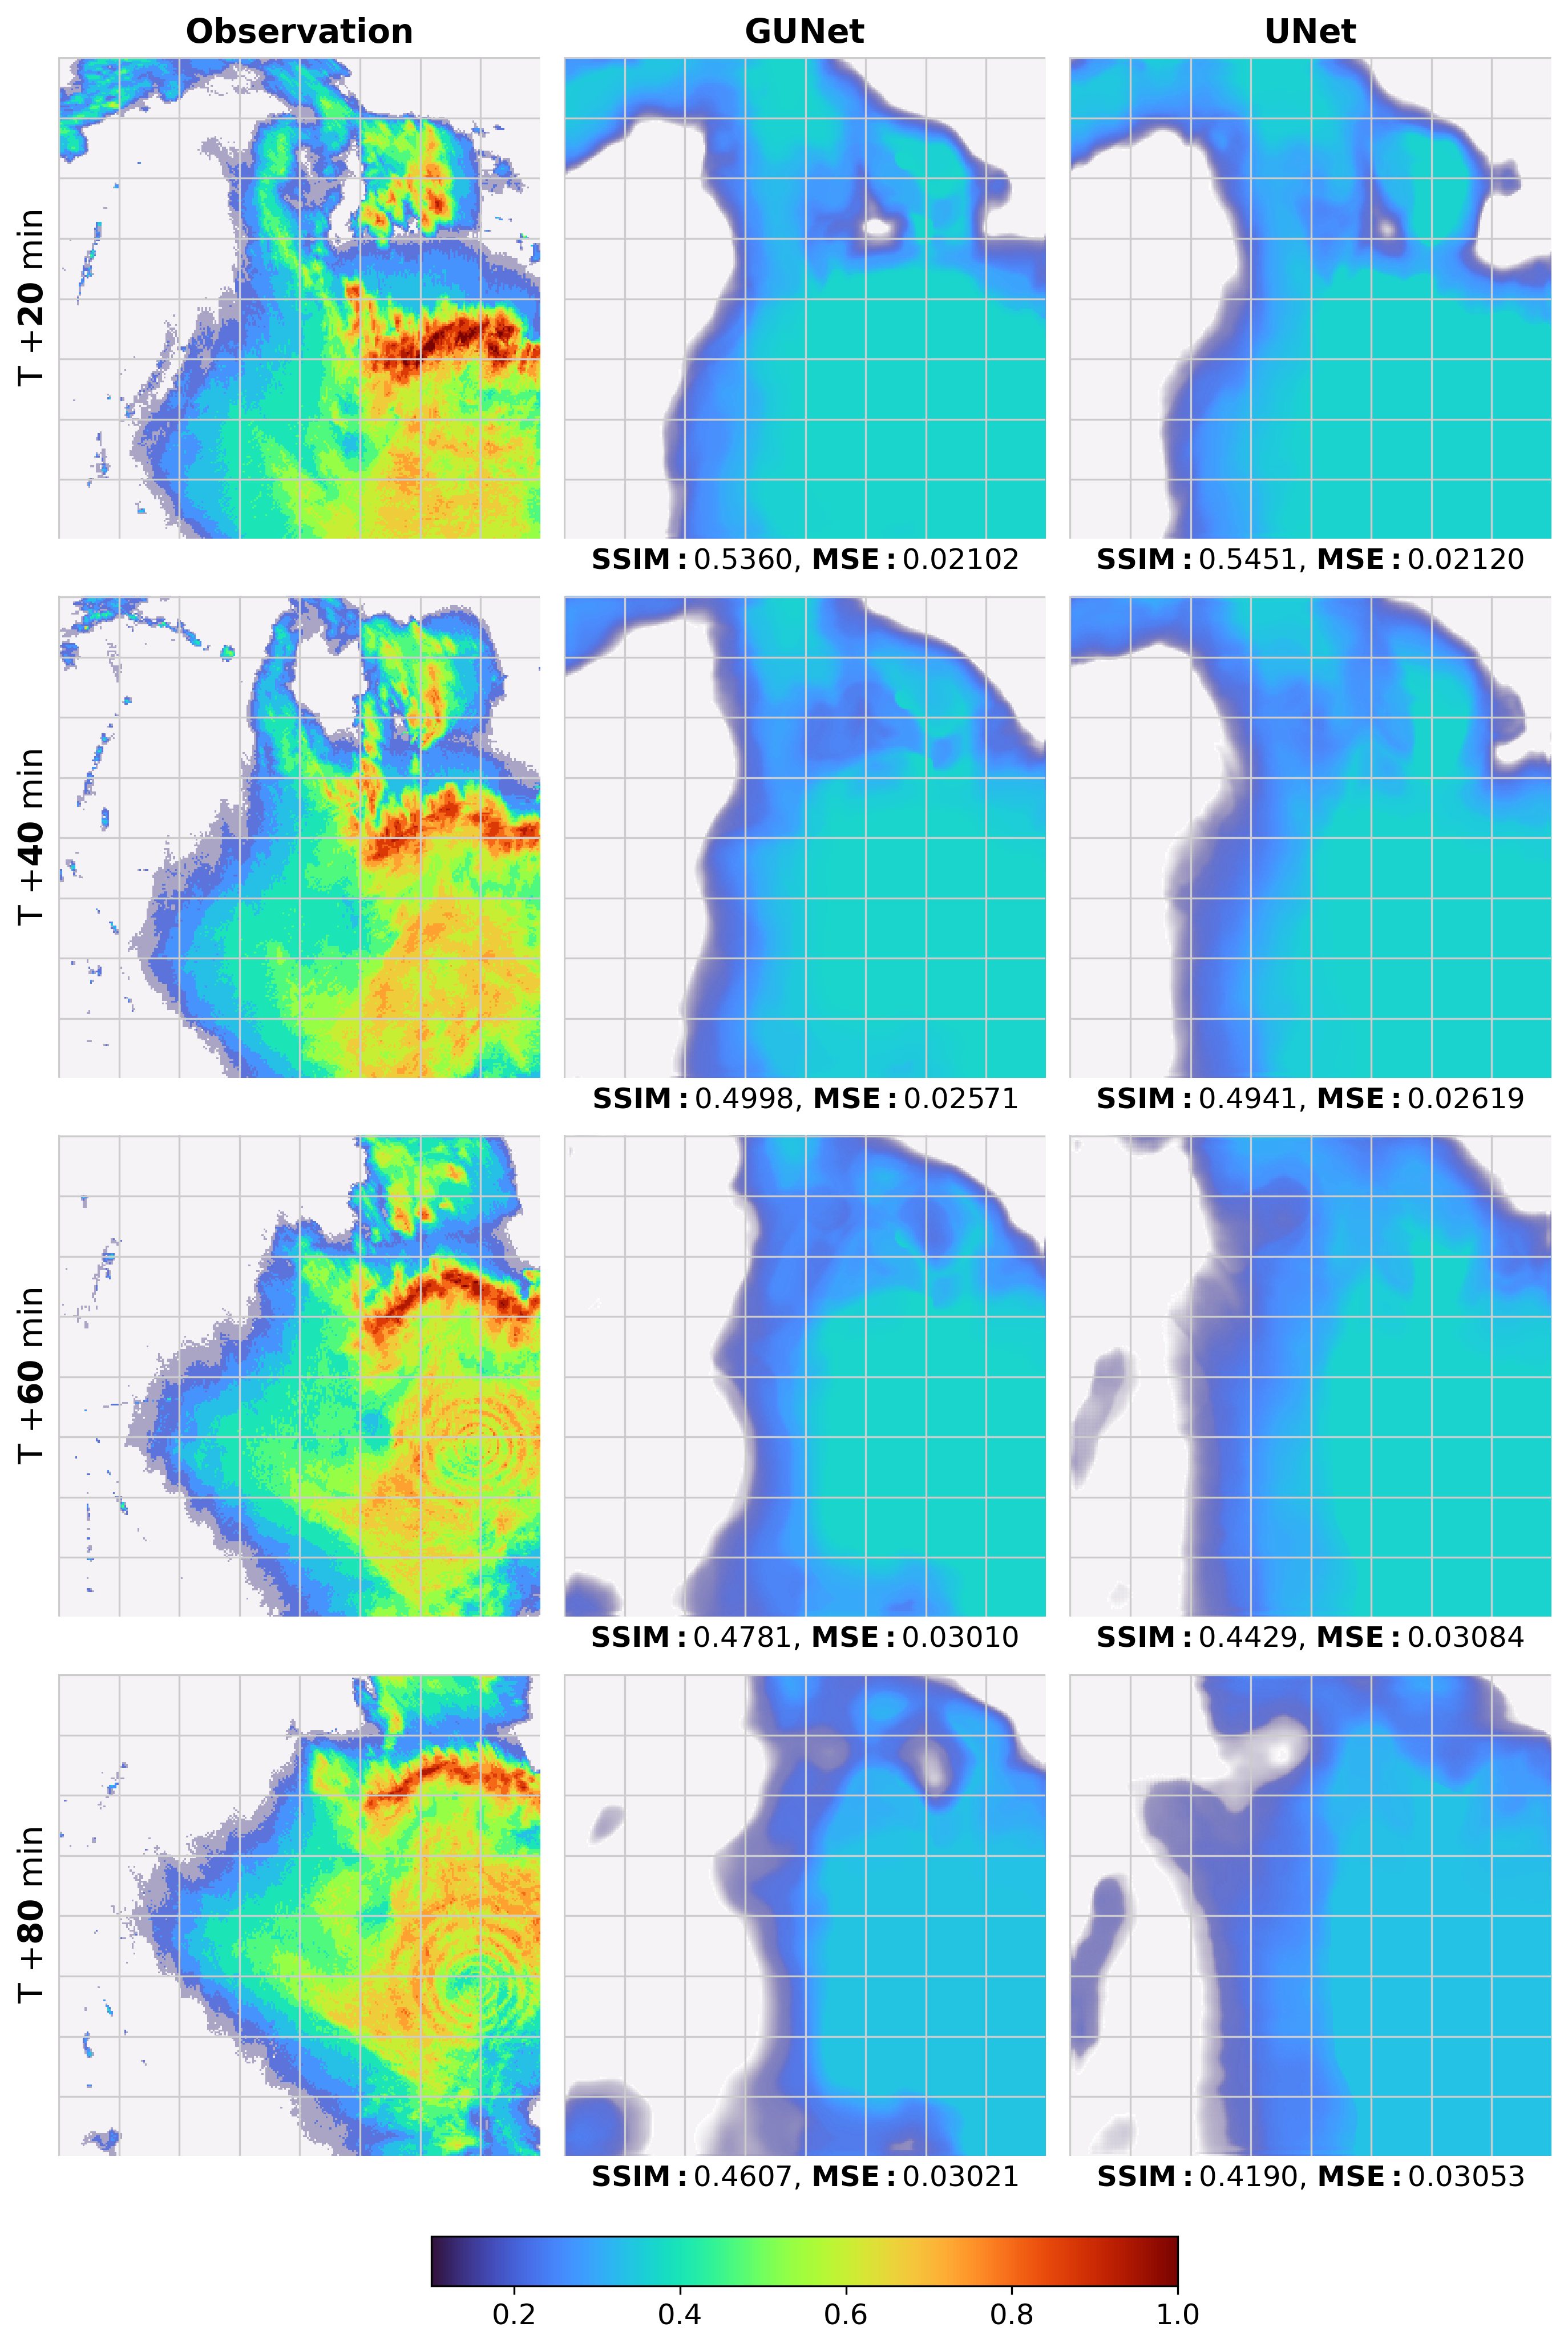
\includegraphics[width=\textwidth]{images/comparison_square_01.jpeg}
%     \caption[Model comparison on radar images with very high intensities]{\label{fig:comparison_01}Model comparison on radar images with very high echo intensities, which are not captured by either one of the models.}
% \end{figure}

\begin{figure}[ht]
    \centering
    \begin{subcaptionblock}[t]{\textwidth}
        \centering
        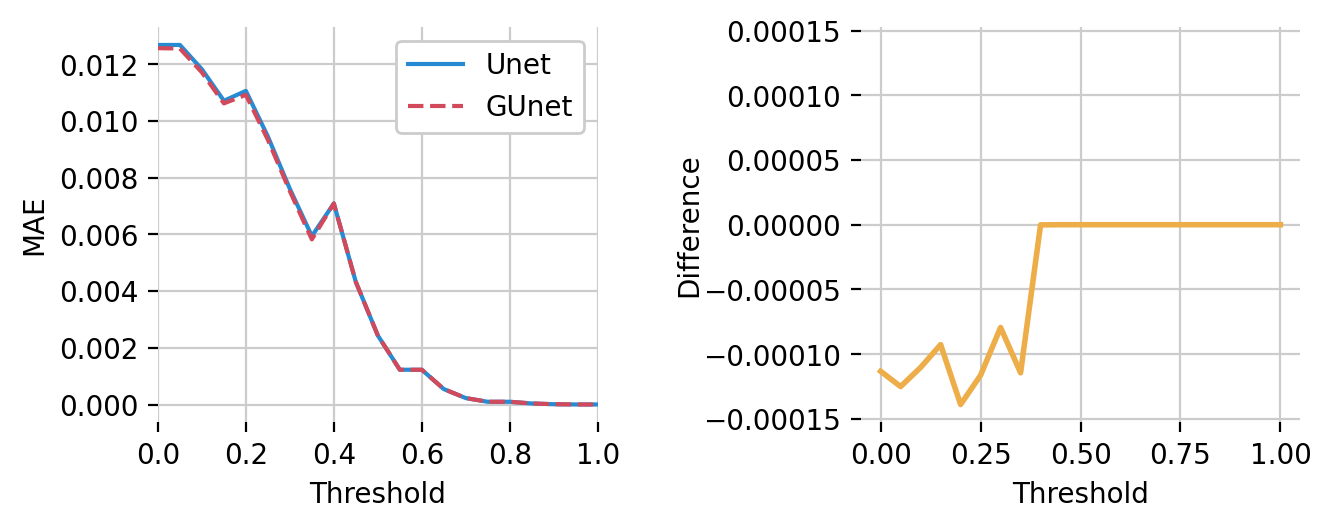
\includegraphics[width=\textwidth]{images/threshold_mae.png}
        \caption[Higher intensity storm prediction metrics]{\label{fig:threshold_mae}Average \gls{MAE} on the test dataset, computed from outputs and targets, which had some values, that were below some threshold, set to 0. Chart on the right shows the difference $\texttt{mae\_gunet} - \texttt{mae\_unet}$. Negative values mean that GUNet had better \gls{MAE}, and positive values that UNet had better \gls{MAE}.}
    \end{subcaptionblock}
    \begin{subcaptionblock}[t]{\textwidth}
        \centering
        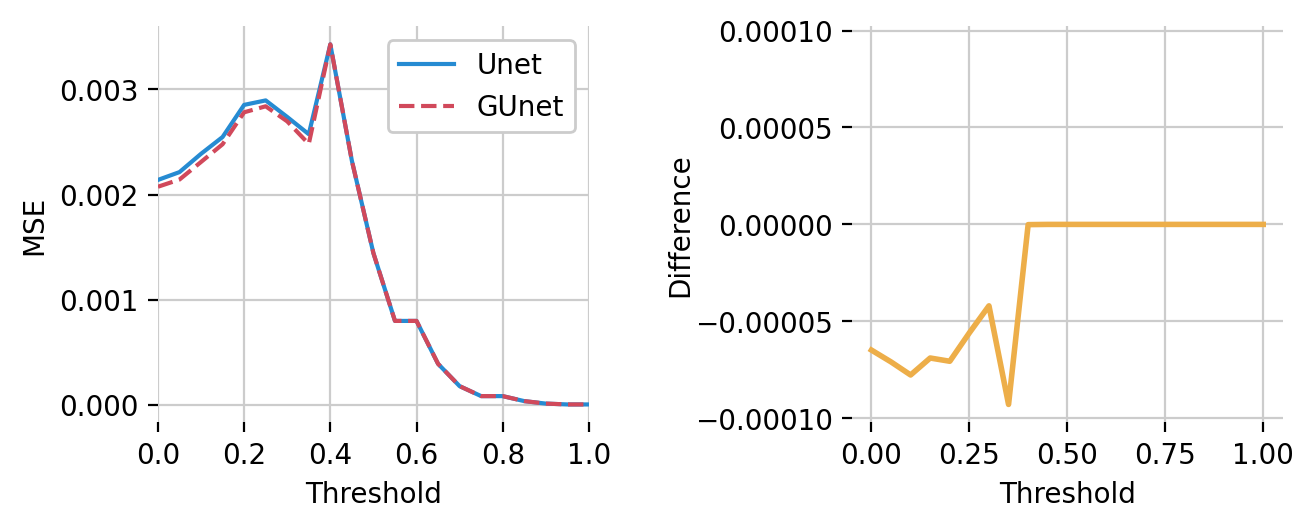
\includegraphics[width=\textwidth]{images/threshold_mse.png}
        \caption[Higher intensity storm prediction metrics]{\label{fig:threshold_mse}Average \gls{MSE} on the test dataset, computed from outputs and targets, which had some values, that were below some threshold, set to 0. Chart on the right shows the difference $\texttt{mse\_gunet} - \texttt{mse\_unet}$. Negative values signify better GUNet \gls{MSE}.}
    \end{subcaptionblock}
\end{figure}


\begin{figure}[ht]
    \centering
    \begin{subcaptionblock}[t]{\textwidth}
        \centering
        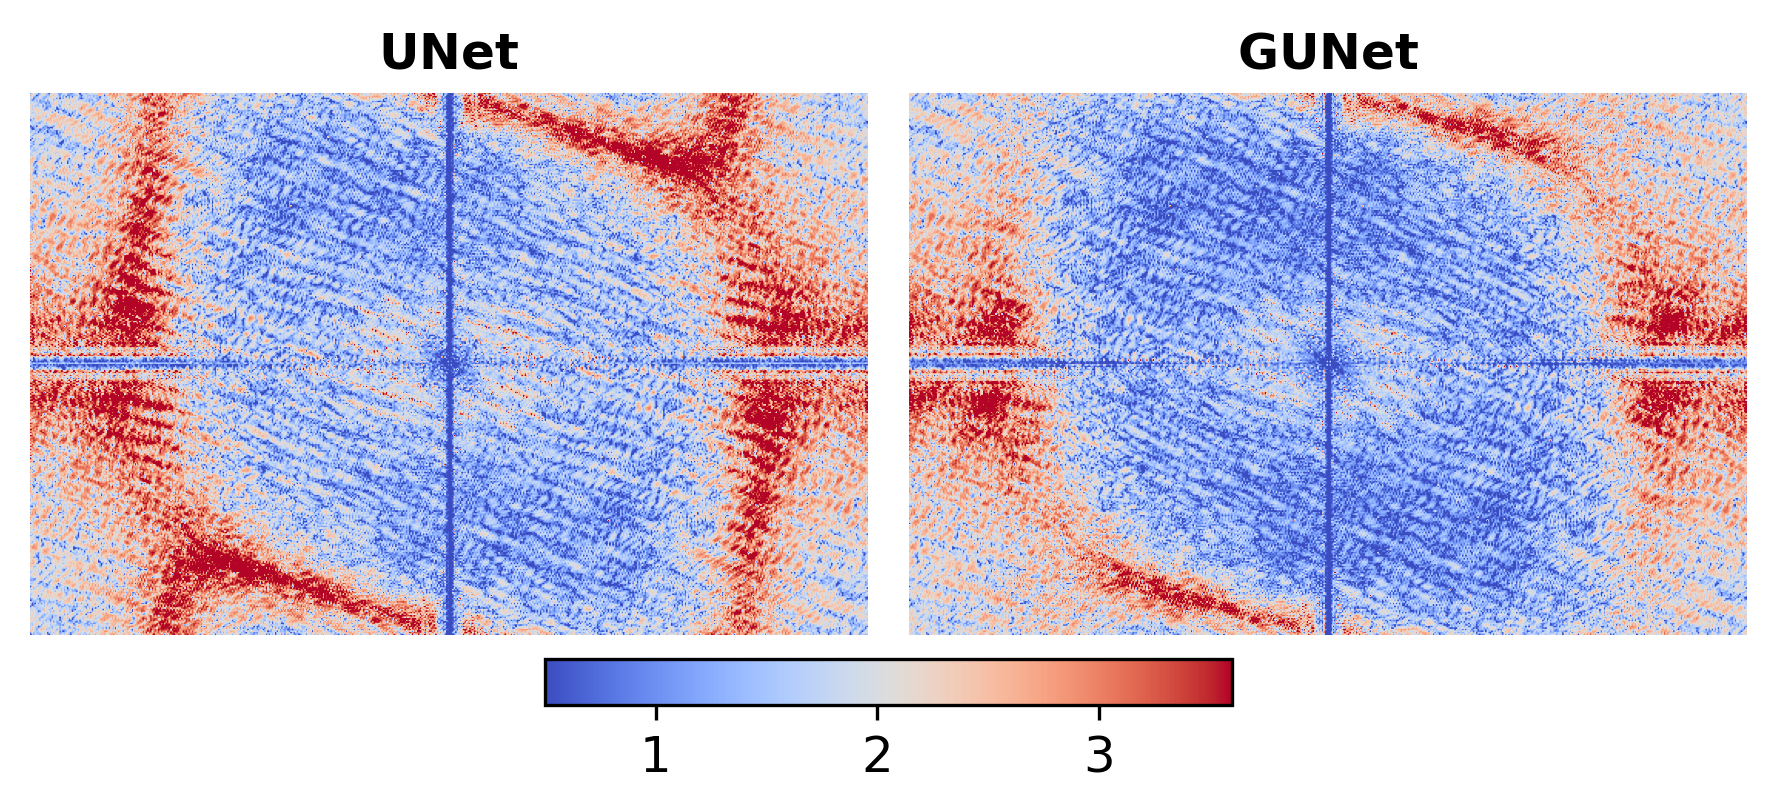
\includegraphics[width=\textwidth]{images/fourier_diff_2.png}
        \caption[Delta of the target and output spectra without smoothing]{\label{fig:fourier_diff_2}Absolute difference between the amplitudes of the average target spectrum $\bar{M}_{\texttt{tgt}}$ and the average output spectra of the models $\bar{M}_{\texttt{UNet}}$ and $\bar{M}_{\texttt{GUNet}}$, on a logarithmic scale. Higher value of a pixel means, that the amplitude at the frequency corresponging to that pixel, differed more from the desired amplitude of average target spectra $\bar{M}_{\texttt{tgt}}$. }
    \end{subcaptionblock}
    \begin{subcaptionblock}[t]{\textwidth}
        \centering
        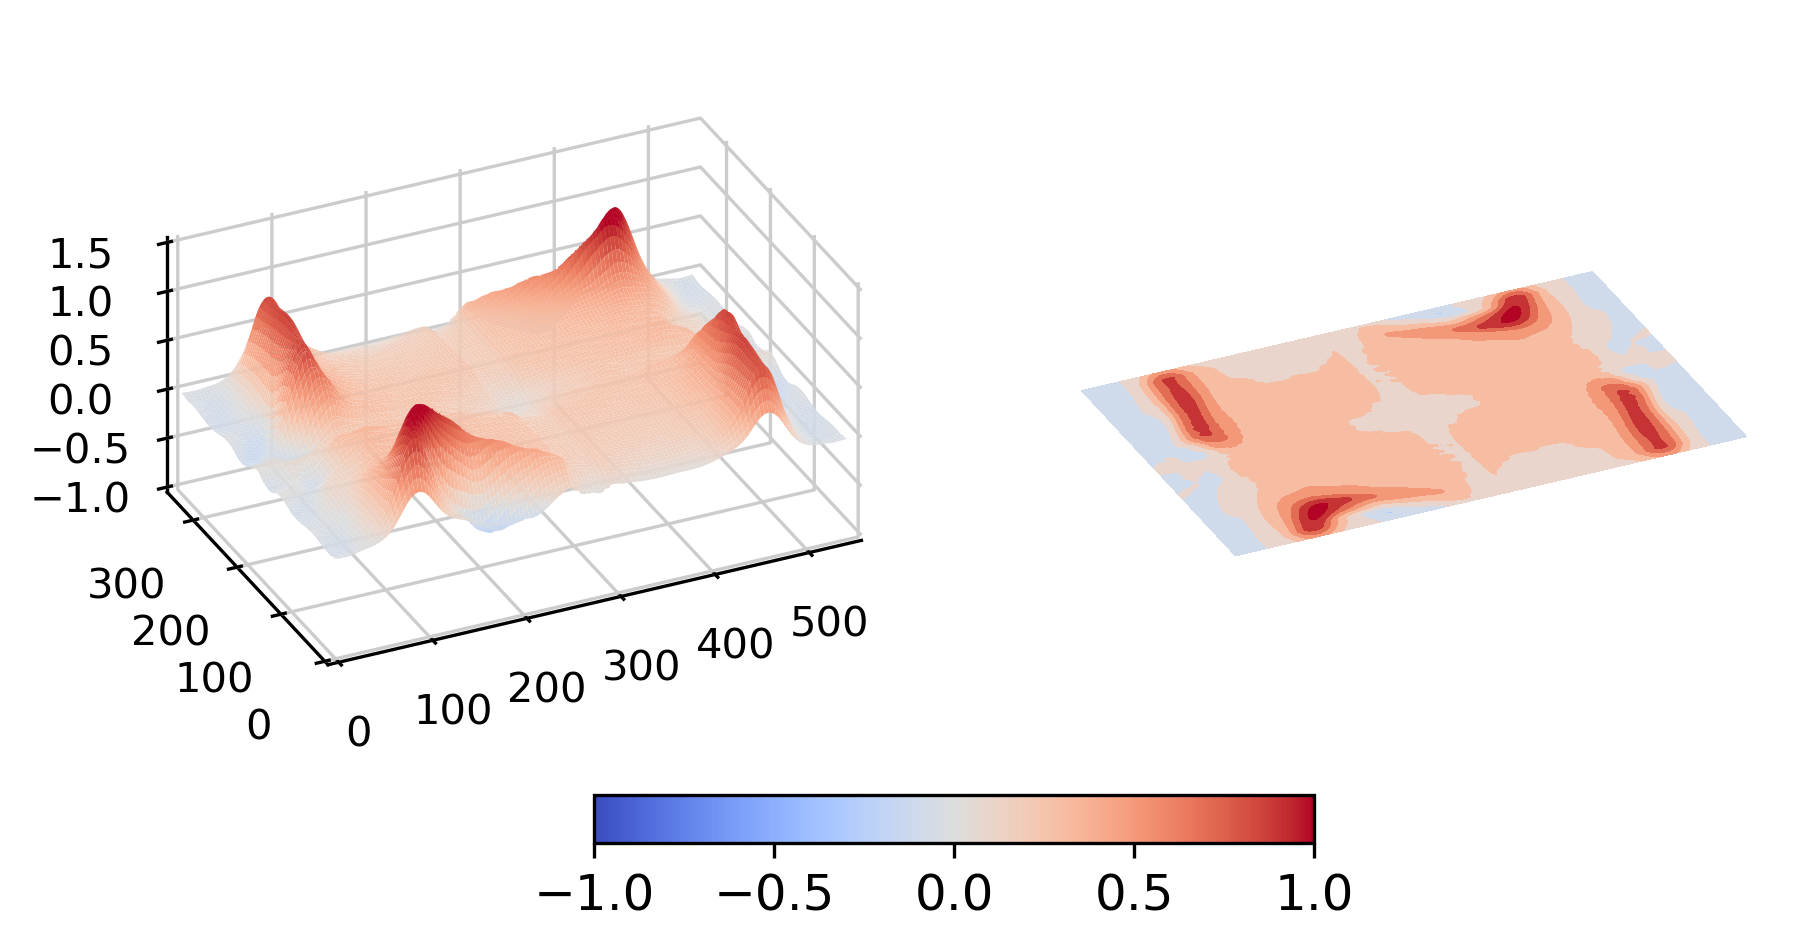
\includegraphics[width=\textwidth]{images/fourier_diff_3.png}
        \caption[Difference in the output spectra of both models]{\label{fig:fourier_diff_3}Amplitudes of the average UNet output spectrum $\bar{M}_{\texttt{UNet}}$ subtracted from the amplitudes of the average GUNet outputs $\bar{M}_{\texttt{GUNet}}$ on a logarithmic scale. Values were passed through moving average with kernel size 32×32. Higher value of a pixel means, that GUNet outputs had higher average amplitude than the UNet outputs, at the frequency corresponging to the given pixel.}
    \end{subcaptionblock}
\end{figure}


\begin{figure}[ht]
    \centering
    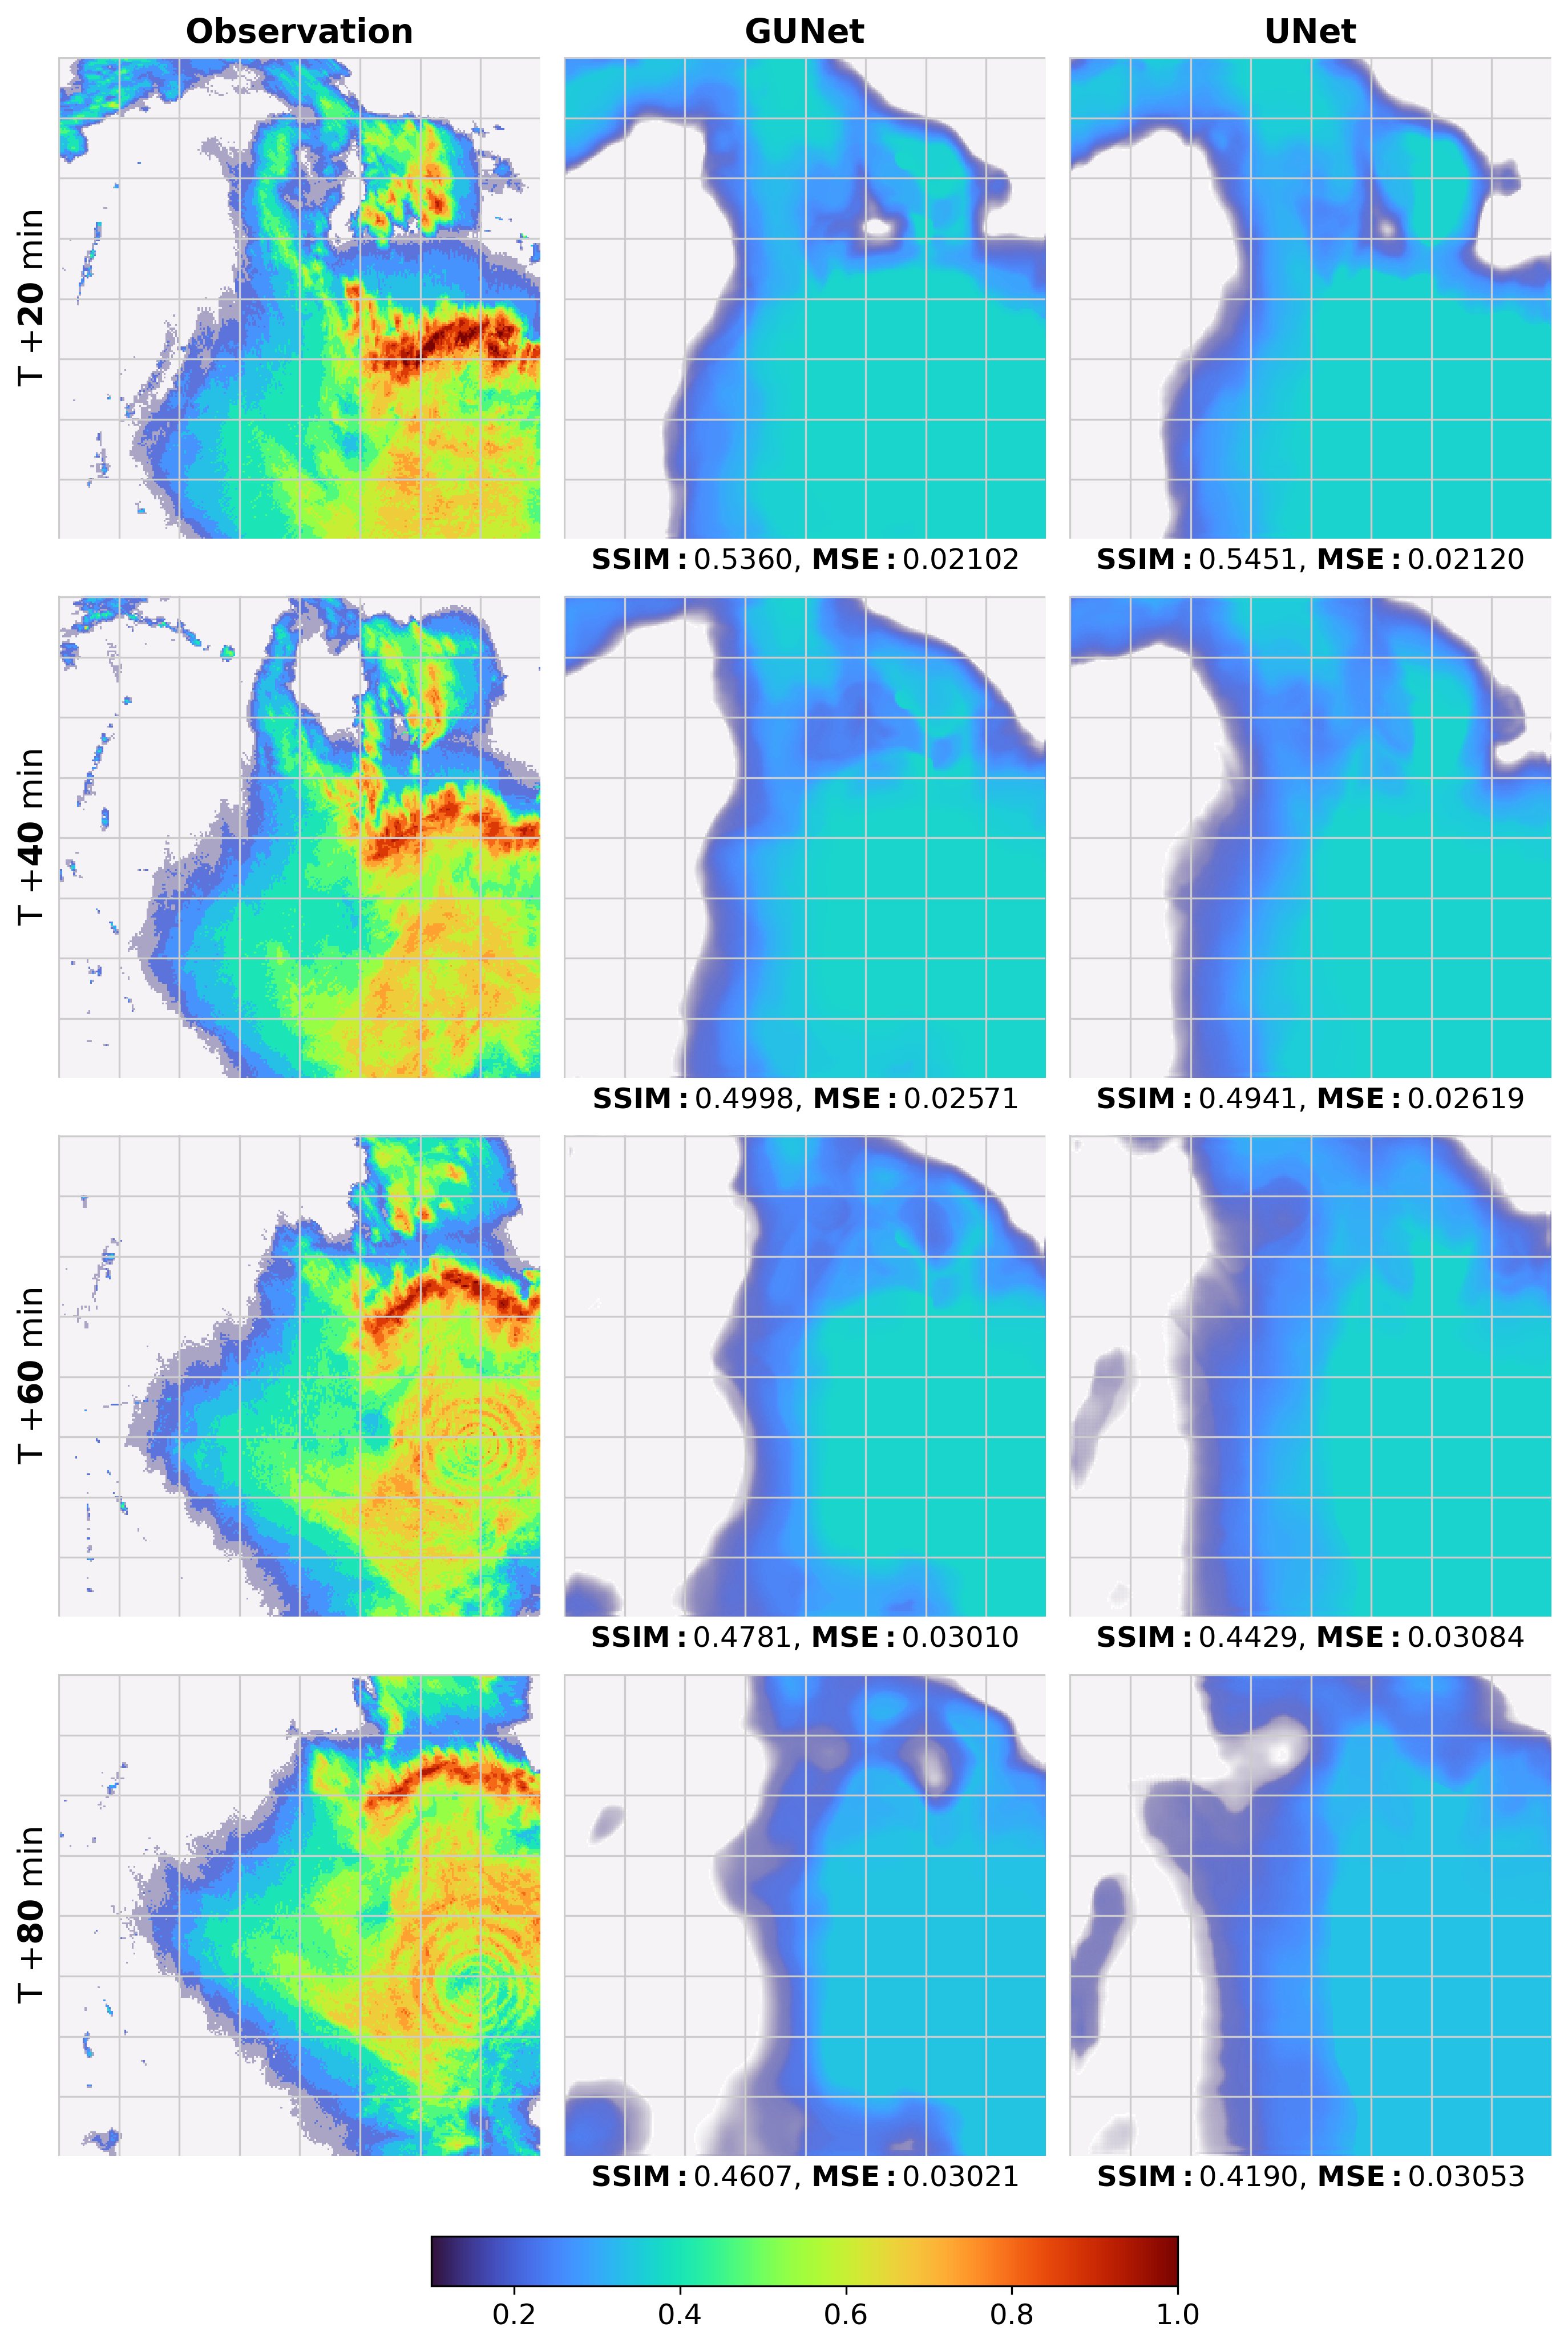
\includegraphics[width=\textwidth]{images/comparison_square_01.png}
    \caption[Comparison of weather predictions of both models (2)]{\label{fig:comparison_01}Model comparison on radar images with very high echo intensities, which are not captured by either one of the models.}
\end{figure}

\begin{figure}[ht]
    \centering
    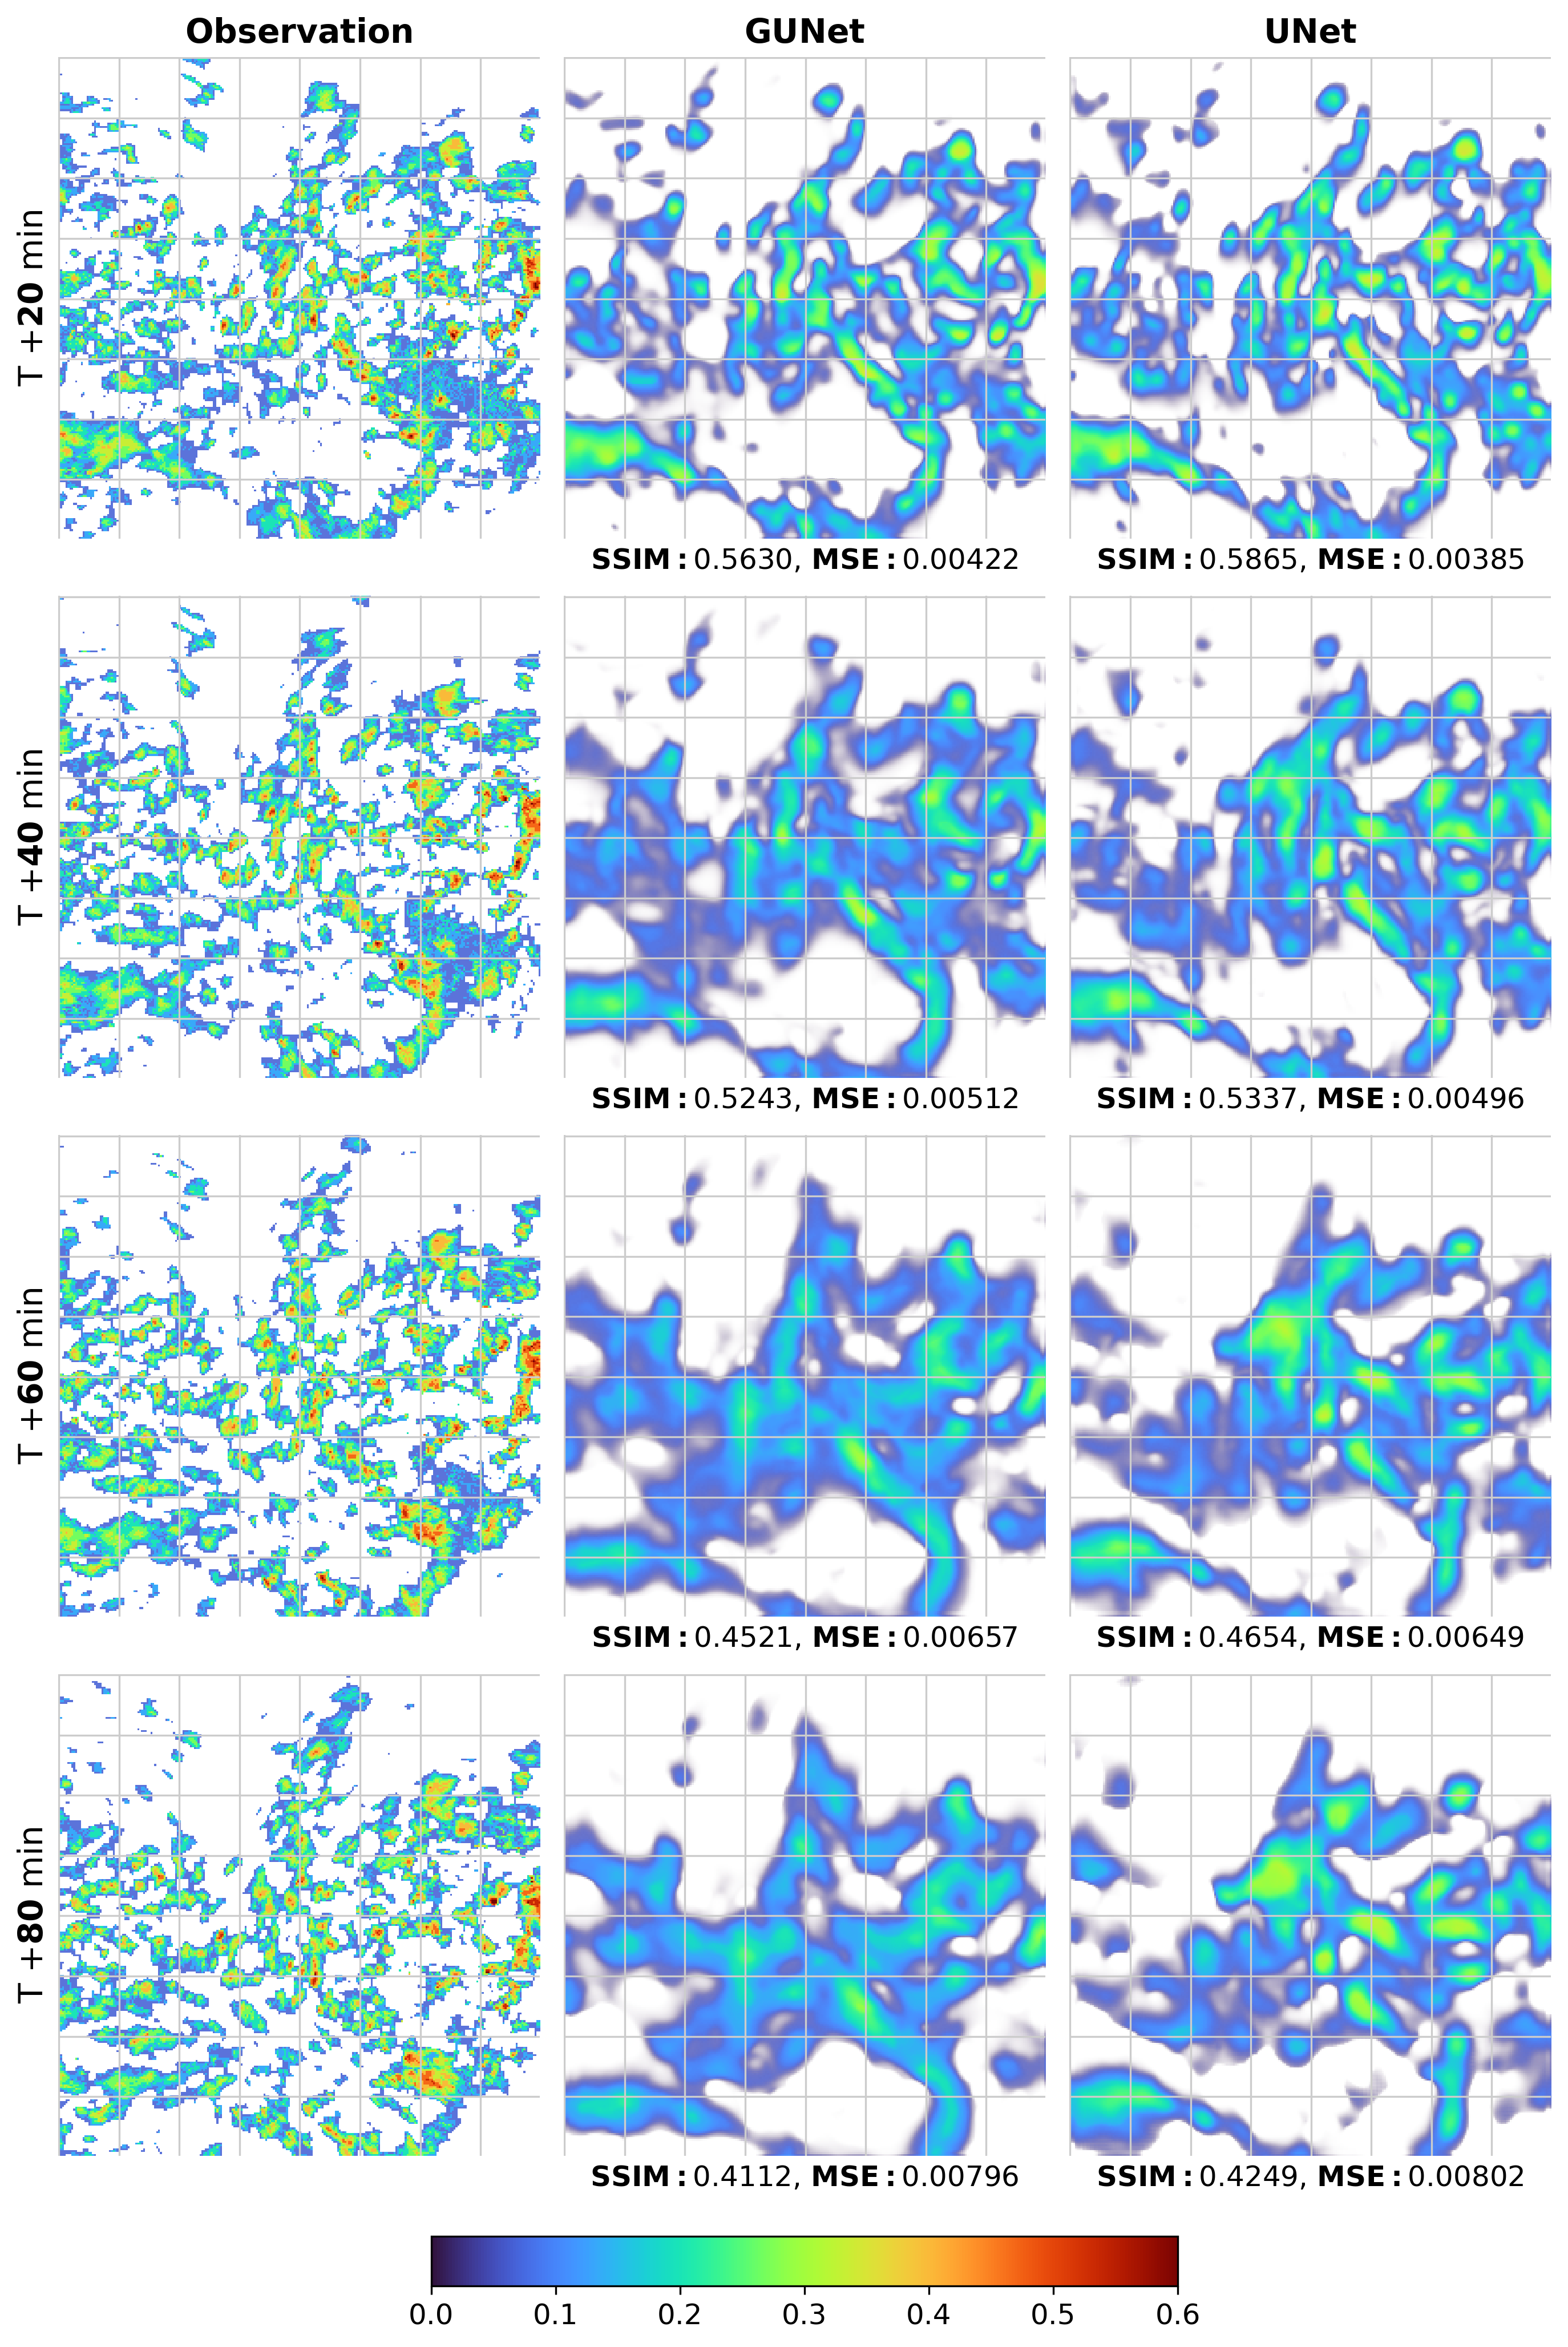
\includegraphics[width=\textwidth]{images/comparison_square_09.png}
    \caption[Comparison of weather predictions of both models (3)]{\label{fig:comparison_09}Model comparison on radar images with complex cloud formations.}
\end{figure}

\begin{figure}[ht]
    \centering
    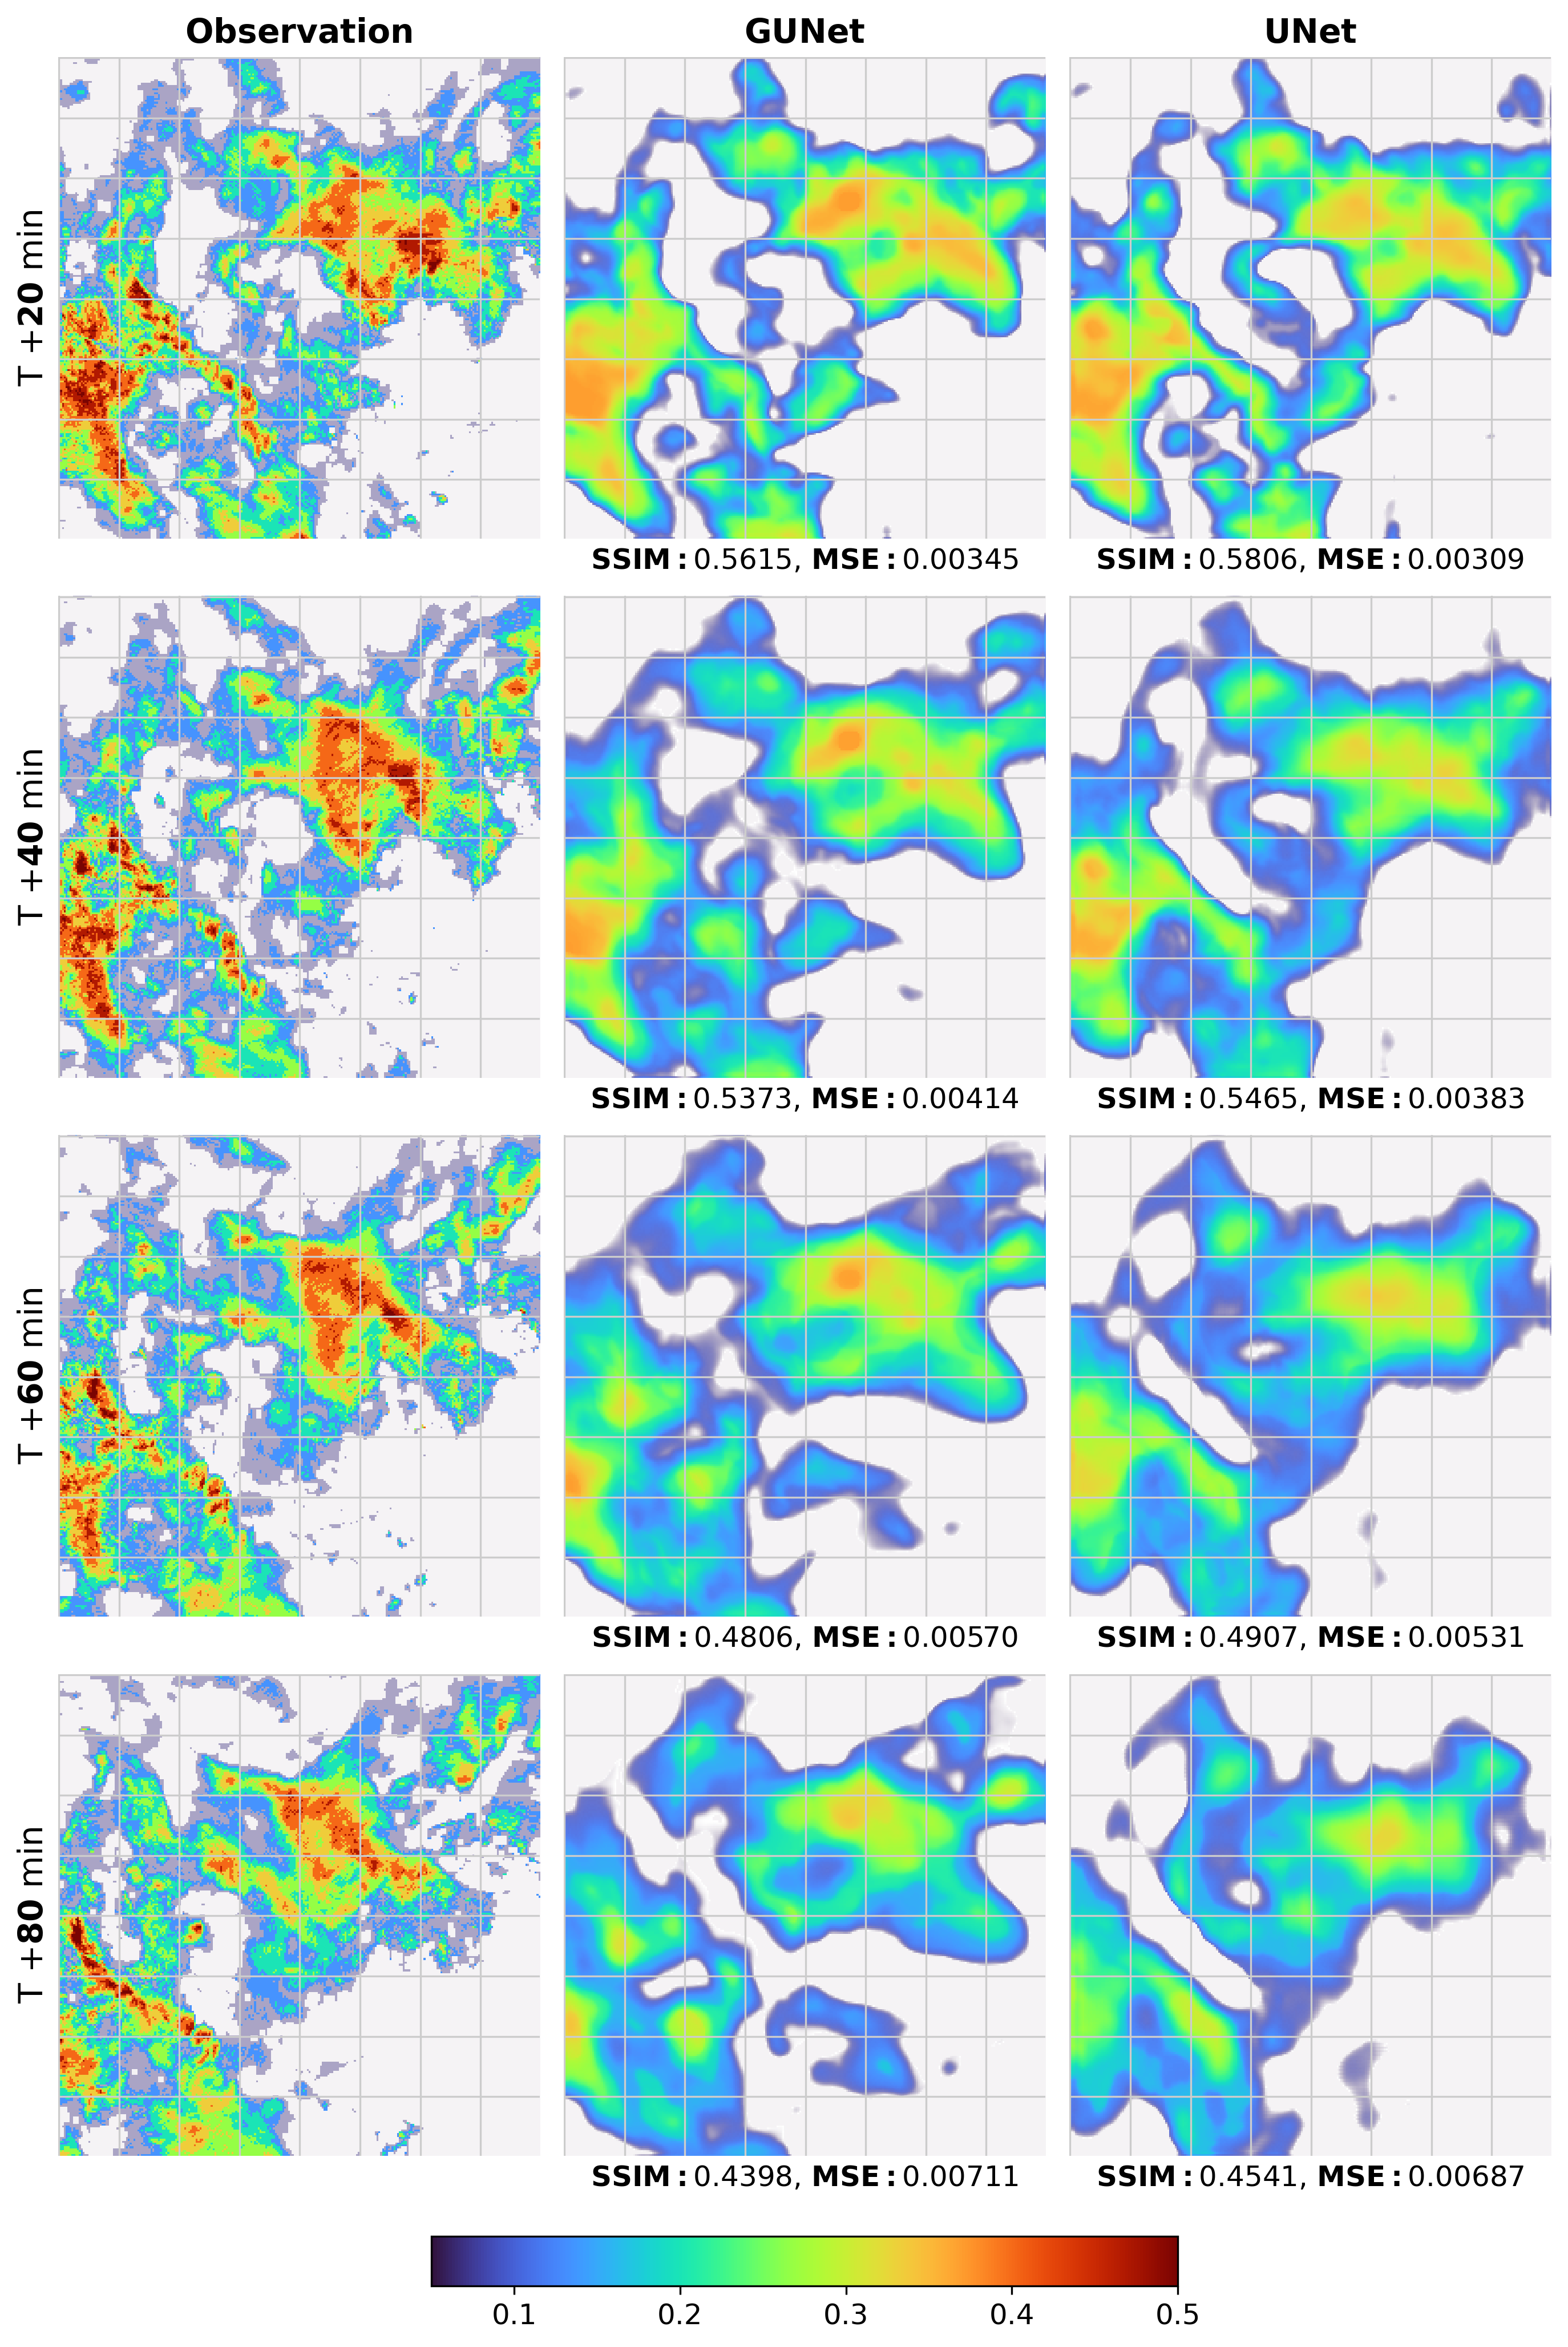
\includegraphics[width=\textwidth]{images/comparison_square_07.png}
    \caption[Comparison of weather predictions of both models.(4)]{\label{fig:comparison_07}}
\end{figure}

\begin{figure}[ht]
    \centering
    \includegraphics[width=\textwidth]{images/comparison_square_04.png}
    \caption[Comparison of weather predictions of both models (5)]{\label{fig:comparison_04}}
\end{figure}

\chapter{Acronyms}
\renewcommand{\glossarysection}[2][]{}
\printglossaries

\chapter{Contents of the Archive}

%change appropriately

\begin{figure}[h]
    \dirtree{%
    .1 docs\DTcomment{the file with CD contents description}.
    .2 wbdcm\DTcomment{implementation sources}.
    .2 chapters\DTcomment{directory containing \LaTeX source code of the chapters}.
    .2 thesis.tex\DTcomment{main \LaTeX source file}
    .2 thesis.pdf\DTcoment{this pdf}
    .1 src\DTcomment{directory containing souce code of the models and }.
    .2 src\DTcomment{directory containing souce code of the models and }.
    .2 src\DTcomment{directory containing souce code of the models and }.
    .1 README.md\DTcomment{file containing information about contents of the archive}.
    }
\end{figure}

\end{document}
